% !TeX encoding = UTF-8
% !TeX spellcheck = sk_SK
\documentclass[]{KKUIzaverecnaPraca}
%% -----------------------------------------------------------------
%% tento subor ma kodovanie utf-8
%%
%% na kompilaciu pouzivajte format pdflatex 
%%
%% V pripade problemov kontaktujte Jána Bušu st. (jan.busa@tuke.sk)
%%
%% edit: Viera Maslej Kresnakova  03/2019
%% -----------------------------------------------------------------
%%
%\usepackage[dvips]{graphicx}
%\DeclareGraphicsExtensions{.eps}
\usepackage{graphicx}
\DeclareGraphicsExtensions{.pdf,.png,.jpg,.mps}
\graphicspath{{figures/}} % priecinok na obrazky
%%
%\usepackage[utf8]{inputenc}  % je v cls-subore
%\usepackage[T1]{fontenc}     % je v cls-subore
\usepackage{fontspec}
\setmainfont{DejaVu Serif}  % or another Unicode font with Slovak support
\usepackage{lmodern,textcase}
\usepackage[slovak]{babel}
\def\refname{Zoznam použitej literatúry}
\usepackage{latexsym}
\usepackage{dcolumn} % zarovnanie cisiel v tabulke podla des. ciarky
\usepackage{hhline}
\usepackage{subcaption} % Package for subfigures
\usepackage{amsmath,amsfonts,amssymb}
\usepackage{nicefrac} % pekne zlomky
\usepackage{upgreek}  % napr. $\upmu\mathrm{m}$ pre mikrometer ...
\usepackage[final]{showkeys} %color%notref%notcite%final
\usepackage[slovak,noprefix]{nomencl}
\makeglossary % prikaz na vytvorenie suboru .glo


% Pouzit v pripade velkeho poctu subsection v tableofcontents
%\makeatletter
%\renewcommand*\l@subsection{\@dottedtocline{2}{1.5em}{3.5em}}
%\newcommand*\l@subsection{\@dottedtocline{2}{1.5em}{2.3em}}
%\newcommand*\l@subsubsection{\@dottedtocline{3}{3.8em}{3.2em}}
%\makeatother


%\def\thefigure{\Roman{section}.\arabic{figure}}
%\usepackage{parskip}% 'zhusti' polozky obsahu

%% Cislovane citovanie
\usepackage[numbers]{natbib}
%%
%% Citovanie podľa mena autora a roku
\usepackage{natbib} %\citestyle{chicago}
% -----------------------------------------------------------------
%% tlač !!!
\usepackage[unicode=true,bookmarksnumbered=true,
bookmarksopen=true,pdfmenubar=true,pdfview=Fit,linktocpage=true,
pageanchor=true,bookmarkstype=toc,pdfpagemode=UseOutlines,
pdfstartpage=1]{hyperref}
\hypersetup{%
baseurl={http://www.tuke.sk/sevcovic},
pdfcreator={pdfcsLaTeX},
pdfkeywords={Optimalizácia, ladenie, neurónové siete, GRU, RNN, hyperparametre, bayesovské vyhľadávanie, náhodné vyhľadávanie, vyhľadávanie v sieti},
pdftitle={Ladenie GRU modelov},
pdfauthor={Nikita Chernysh},
pdfsubject={Semestrálna práca}
} 

%% !!!  nehodiace zakomentujte !!!!
%\dippraca{Diplomová práca}
%\bakpraca{Bakalárska práca}
%%
\nazov{Ladenie GRU modelov}
%% ked praca nema 'podnazov' zakomentujte nasledujuci riadok
%% alebo polozku nechajte prazdnu
\podnazov{}
\jazyk{Slovenský}
% anglicky nazov
\title{Ladenie GRU modelov}
\autor{Študent: Nikita Chernysh}
\veduciprace{Ing. Miroslava Matejová}
\konzultanta{Ing. Miroslava Matejová}
%\konzultantb{RNDr.~Marián~Čierny, DrSc.}
\titul{Študent}
\univerzita{Technická univerzita v~Košiciach}
\fakulta{Fakulta elektrotechniky a informatiky}
\skratkafakulty{FEI}
\katedra{Katedra kybernetiky a umelej inteligencie}
\skratkakatedry{KKUI}
\odbor{Inteligentné systémy}
\specializacia{Inteligentné systémy}

\abstrakt{Táto práca sa zaoberá hľadaním, optimalizáciou a testovaním hyperparametrov modelu rekurentnej neurónovej siete (RNN) založeného na architektúre GRU (Gated Recurrent Unit). Cieľom bolo vyvinúť všeobecný algoritmus schopný pracovať s ľubovoľnými dátami, pričom všetky metriky hodnotenia a výpočty boli implementované s využitím základných matematických knižníc. Výnimku tvorí samotný GRU model. Praktické overenie navrhnutého prístupu bolo realizované na reálnom datasete o prenájmoch bicyklov v Londýne. Výsledky experimentov potvrdzujú efektivitu vybraných metód optimalizácie hyperparametrov (grid search, random search a Bayesian search).}
\klucoveslova{Ladenie, GRU, RNN, hyperparametre, bayesovské vyhľadávanie, náhodné vyhľadávanie, vyhľadávanie v sieti}

\abstrakte{This work focuses on finding, optimizing, and testing hyperparameters of a recurrent neural network (RNN) model based on the GRU (Gated Recurrent Unit) architecture. The goal was to develop a universal algorithm capable of working with arbitrary datasets, with all evaluation metrics and calculations implemented using basic mathematical libraries. The exception is the GRU model itself. Practical verification of the proposed approach was conducted on a real-world dataset of bike rentals in London. Experimental results confirm the effectiveness of selected hyperparameter optimization methods (grid search, random search, and Bayesian search).}
\keywords{Optimization, debugging, neural networks, GRU, RNN, hyperparameters, bayesian search, random search, grid search}

\datumodovzdania{9.~5.~2025}
\datumobhajoby{14.~5.~2025}
\mesto{Košice}
\pocetstran{\pageref{page:posledna}}
\kategoria{Semestrálna práca}

\begin{document}
\renewcommand{\figurename}{Obrázok}	
\renewcommand\theHfigure{\theHsection.\arabic{figure}}
\renewcommand\theHtable{\theHsection.\arabic{table}}
\bibliographystyle{dcu}

\prvastrana

\titulnastrana

%\analytickylist


%\errata % zaciatok erraty
%Ak je potrebné, autor na tomto mieste opraví chyby, ktoré našiel po
%vytlačení práce. Opravy sa uvádzajú takým písmom, akým je napísaná
%práca. Ak zistíme chyby až po vytlačení a zviazaní práce, napíšem
%erráta na samostatný lístok, ktorý vložíme na toto miesto. Najlepšie je
%lístok prilepiť \citep{kat}.
%
%Forma:
%
%%\tabcolsep=10pt
%\begin{table}[!hb]
%	\centering
%	\begin{tabular}{|c|c|c|c|}\hline
%Strana & Riadok & Chybne & Správne \\\hline\hline
%12 & 6 & publikácia & prezentácia \\\hline
%22 & 23 & internet & intranet \\\hline
%& & & \\\hline
%& & & \\\hline
%	\end{tabular}
%\end{table}
%\kerrata % koniec erraty

\abstraktsk % abstrakt v SK 

\abstrakteng % abstrakt v ENG

\kabstrakt % koniec abstraktov, nova strana

% Na tomto mieste bude vložené zadanie diplomovej práce
\zadanieprace

\cestnevyhlasenie
% Niektorí autori metodických príručiek o~záverečných prácach sa
% nazdávajú, že takéto vyhlásenie je zbytočné, nakoľko povinnosť
% vypracovať záverečnú prácu samostatne, vyplýva študentovi zo zákona a na autora práce sa vzťahuje autorský zákon.

%\podakovanie
%Na tomto mieste môže byť vyjadrenie poďakovania napr. vedúcemu
%diplomovej práce, resp. konzultantom, za pripomienky a~odbornú pomoc
%pri vypracovaní diplomovej práce.
%
%Na tomto mieste môže byť vyjadrenie poďakovania napr. vedúcemu
%diplomovej práce, respektíve konzultantom, za pripomienky a~odbornú
%pomoc pri vypracovaní diplomovej práce.
%
%Na tomto mieste môže byť vyjadrenie poďakovania napr. vedúcemu
%diplomovej práce alebo konzultantom za pripomienky a~odbornú pomoc pri
%vypracovaní diplomovej práce.
%\kpodakovania

\predhovor
Táto semestrálna práca bola vypracovaná v rámci predmetu „Strojové učenie“ na Fakulte elektrotechniky a informatiky Technickej univerzity v Košiciach. Jej hlavným cieľom bolo prakticky aplikovať nadobudnuté vedomosti z oblasti strojového učenia na implementáciu rekurentnej neurónovej siete založenej na architektúre GRU (Gated Recurrent Unit), a zároveň splniť všetky stanovené obmedzenia – najmä zákaz využívania hotových knižničných implementácií algoritmov a metrík.

Počas práce bol kladený dôraz na všeobecnú aplikovateľnosť algoritmu na akýkoľvek dataset, nezávisle od jeho štruktúry či pôvodu. Navyše, implementácia všetkých metrík, výpočtov a pomocných nástrojov bola realizovaná výlučne pomocou základných matematických knižníc ako \texttt{numpy} a \texttt{pandas}. Výnimku tvorila iba samotná architektúra GRU, ktorá bola implementovaná s využitím knižnice \texttt{PyTorch}, keďže vytvorenie GRU blokov od základov by výrazne presahovalo rozsah zadania.

Reálny dataset použitý na experimenty predstavuje historické záznamy o prenájme bicyklov v Londýne. Práca zahŕňa kompletný životný cyklus vývoja modelu – od predspracovania dát, cez návrh modelu, optimalizáciu hyperparametrov (s využitím viacerých stratégií), až po vyhodnotenie výsledkov a ich vizualizáciu. Cieľom tejto práce bolo nielen technicky zvládnuť implementáciu, ale aj získať hlbšie porozumenie fungovaniu GRU modelov v kontexte sekvenčných dát.

Touto cestou by som sa chcel poďakovať vyučujúcim predmetu za odborné vedenie a podporu počas semestra.
\kpredhovoru

\thispagestyle{empty}
\tableofcontents
\newpage

\thispagestyle{empty}

{	\makeatletter
	\renewcommand{\l@figure}{\@dottedtocline{1}{1.5em}{3.5em}}
	\makeatother
	\listoffigures}

%\addcontentsline{toc}{section}{\numberline{}Zoznam obrázkov}
%\listoffigures


\newpage

\thispagestyle{empty}
%\addcontentsline{toc}{section}{\numberline{}Zoznam tabuliek}
\listoftables
\newpage

\thispagestyle{empty}
%\addcontentsline{toc}{section}{\numberline{}Zoznam symbolov a skratiek}
%\printglossary % vlozenie zoznamu skratiek a symbolov
\newpage

%\addcontentsline{toc}{section}{\numberline{}Slovník termínov}
\slovnikterminov

\begin{description}
    \item [Strojové učenie (Machine Learning)] – Oblasť umelej inteligencie, ktorá sa zaoberá tvorbou algoritmov schopných učiť sa z dát a zlepšovať svoje výstupy bez nutnosti explicitného programovania všetkých krokov.

    \item [Rekurentná neurónová sieť (RNN)] – Typ neurónovej siete navrhnutý na spracovanie sekvenčných dát. Umožňuje uchovávanie informácií z predchádzajúcich stavov prostredníctvom vnútorných pamäťových štruktúr.

    \item [GRU (Gated Recurrent Unit)] – Variant rekurentnej neurónovej siete, ktorý využíva mechanizmy brán (update a reset gate) na efektívnejšie učenie dlhodobých závislostí a zmierňuje problém miznúcich gradientov.

    \item [Hyperparameter] – Parameter, ktorý nie je učený modelom, ale je nastavený pred samotným tréningom. Zahŕňa napríklad veľkosť skrytého stavu, počet vrstiev alebo rýchlosť učenia.

    \item [Optimalizácia hyperparametrov] – Proces hľadania najvhodnejšej kombinácie hyperparametrov, ktorý vedie k zlepšeniu výkonnosti modelu na validačných dátach.

    \item [MAE (Mean Absolute Error)] – Priemerná absolútna chyba medzi predikovanými a skutočnými hodnotami. Udáva sa v rovnakých jednotkách ako cieľová premenná.

    \item [MSE (Mean Squared Error)] – Priemer štvorcov rozdielov medzi predikciami a skutočnými hodnotami. Zvýrazňuje väčšie odchýlky.

    \item [RMSE (Root Mean Squared Error)] – Druhá odmocnina z MSE. Interpretovateľná v rovnakých jednotkách ako cieľová premenná, citlivejšia na veľké chyby.

    \item [R\textsuperscript{2} (Koeficient determinácie)] – Miera vysvetlenej variability cieľovej premennej modelom. Hodnoty blízke 1 indikujú vysokú presnosť modelu.

    \item [MAPE (Mean Absolute Percentage Error)] – Priemerná absolútna percentuálna chyba. Vyjadruje chybu v percentách voči skutočným hodnotám.

    \item [SMAPE (Symmetric Mean Absolute Percentage Error)] – Symetrická verzia MAPE, ktorá redukuje skreslenie pri malých hodnotách.

    \item [Explained Error (Explained Variance Score)] – Ukazovateľ, do akej miery variabilita predikcií vysvetľuje variabilitu skutočných hodnôt.

    \item [Peak Error] – Maximálna absolútna chyba v rámci celej testovacej množiny. Používa sa na odhalenie najväčších extrémnych odchýlok.

    \item [Sekvenčné dáta] – Typ dát, kde je dôležité poradie záznamov. Typickými príkladmi sú časové rady alebo textové reťazce.

    \item [Tréningová množina] – Časť dát použiteľná na učenie modelu.

    \item [Testovacia množina] – Časť dát určená na nezávislé vyhodnotenie výkonnosti modelu po trénovaní.

    \item [Validácia] – Proces priebežného vyhodnocovania modelu na samostatnej množine za účelom výberu najvhodnejších hyperparametrov a predchádzania pretrénovania.
\end{description}

\kslovnikterminov

% !TeX encoding = UTF-8
% !TeX spellcheck = sk_SK
% !TeX root=tukedip.tex
\setcounter{page}{1}
\setcounter{equation}{0}
\setcounter{figure}{0}
\setcounter{table}{0}

\section*{Úvod}
\addcontentsline{toc}{section}{\numberline{}Úvod}
Význam strojového učenia neustále narastá, čo vedie k vzniku množstva rôznych modelov a architektúr schopných riešiť široké spektrum úloh, od predikcie časových radov po spracovanie prirodzeného jazyka. Medzi najpopulárnejšie modely patria rekurentné neurónové siete (RNN), ktoré sú vhodné na spracovanie sekvenčných dát vďaka schopnosti pamätať si predchádzajúce vstupy. Jednou z efektívnych a rozšírených architektúr RNN je Gated Recurrent Unit (GRU).

Táto práca sa zameriava na problematiku optimalizácie hyperparametrov GRU modelov. Správny výber a nastavenie hyperparametrov má zásadný vplyv na výkonnosť a presnosť modelu. Implementácia musí byť dostatočne univerzálna na použitie s rôznymi dátovými množinami bez nutnosti zásadných úprav kódu. V rámci zadania bolo nutné všetky metriky hodnotenia implementovať manuálne, čo umožňuje hlbšie pochopenie a kontrolu nad celým procesom učenia.
% !TeX encoding = UTF-8
% !TeX spellcheck = sk_SK
% !TeX root=tukedip.tex
\section{Formulácia úlohy}
Hlavným cieľom tejto práce bolo navrhnúť, implementovať a otestovať algoritmus pre vyhľadávanie, optimalizáciu a hodnotenie hyperparametrov modelu RNN využívajúceho GRU architektúru. Konkrétne boli stanovené nasledovné ciele:

\begin{itemize}
\item Implementovať univerzálny algoritmus pre optimalizáciu hyperparametrov GRU, schopný aplikácie na ľubovoľný dataset.
\item Vytvoriť manuálne implementované metriky hodnotenia pomocou knižníc numpy a pandas.
\item Overiť algoritmus na reálnych dátach o prenájme bicyklov v Londýne.
\item Porovnať efektívnosť rôznych metód optimalizácie hyperparametrov, konkrétne grid search, random search a Bayesian search.
\end{itemize}
% !TeX root=tukedip.tex
% !TeX encoding = UTF-8
% !TeX spellcheck = sk_SK
%\section{Analýza}

\section{Analýza existujúcich riešení a metód}

V tejto kapitole sa zaoberáme analýzou existujúcich prístupov k optimalizácii hyperparametrov rekurentných neurónových sietí s dôrazom na architektúru GRU. Podrobne skúmame hlavné metódy optimalizácie hyperparametrov a analyzujeme ich výhody a nevýhody v kontexte použitia na rôznych dátových množinách.

\subsection{Metódy optimalizácie hyperparametrov}

Optimálne nastavenie hyperparametrov je kľúčové pre dosiahnutie vysokej presnosti modelov strojového učenia. Existujú rôzne prístupy na riešenie tejto úlohy:

\textbf{Grid Search} predstavuje systematické skúmanie vopred definovanej množiny hyperparametrov, kde každý parameter je testovaný v rôznych kombináciách s ostatnými. Táto metóda je jednoduchá na implementáciu, ale neefektívna pri veľkom počte hyperparametrov, keďže počet potrebných výpočtov rastie exponenciálne.

\textbf{Random Search} vykonáva náhodný výber kombinácií hyperparametrov z definovaného rozsahu. Táto metóda je efektívnejšia ako grid search v prípadoch s veľkým počtom parametrov, pretože poskytuje širšie pokrytie priestoru hyperparametrov s menším počtom iterácií.

\textbf{Bayesian Search} využíva Bayesovské metódy na riadenie výberu kombinácií hyperparametrov. Táto metóda postupne zlepšuje svoj výber na základe predchádzajúcich výsledkov a je efektívna najmä pri zložitých modeloch, kde tradičné metódy optimalizácie môžu byť neefektívne.

Postup optimalizácie bol nasledovný: najprv bol vykonaný random a Bayesian search na rovnakom rozsahu hyperparametrov. Následne boli tri najlepšie sady hyperparametrov z oboch metód kombinované a pomocou grid search bola nájdená najlepšia výsledná kombinácia. Tento prístup umožnil efektívne zúženie priestoru hľadania a zvýšenie presnosti finálneho výberu hyperparametrov.

\subsection{Analýza dostupných metrík hodnotenia}

Pre vyhodnotenie výkonu modelov strojového učenia sa používajú rôzne metriky. V rámci tejto práce sme manuálne implementovali niekoľko štandardných metrík (\ref{sec:metrics}) s využitím knižníc numpy a pandas:

\begin{itemize}
\item \textbf{MSE (Mean Squared Error)}: Priemerná štvorcová chyba meria priemernú veľkosť chyby medzi predikovanými a reálnymi hodnotami.
\item \textbf{MAE (Mean Absolute Error)}: Priemerná absolútna chyba, robustnejšia metrika voči odľahlým hodnotám.
\item \textbf{RMSE (Root Mean Squared Error)}: Odmocnina z MSE, poskytuje chybu v jednotkách pôvodnej veličiny, čím zlepšuje interpretovateľnosť výsledkov.
\item \textbf{R-squared (koeficient determinácie)}: Udáva mieru zhody medzi modelom a dátami, pričom vyššie hodnoty naznačujú lepšiu predikčnú schopnosť.
\item \textbf{MAPE (Mean Absolute Percentage Error)}: Priemerná absolútna percentuálna chyba, vhodná na vyhodnotenie relatívnej veľkosti chyby.
\item \textbf{sMAPE (Symmetric Mean Absolute Percentage Error)}: Symetrická verzia MAPE, vhodná pre symetrické posúdenie chyby.
\item \textbf{Explained Variance}: Vyjadruje podiel vysvetlenej variancie modelom oproti celkovej variancii dát.
\item \textbf{Peak Error}: Udáva najväčšiu chybu medzi predikciou a reálnymi hodnotami, dôležitá pre analýzu kritických chýb.
\end{itemize}

Tieto metriky poskytujú jasný pohľad na presnosť a efektivitu vyvinutého algoritmu v rámci tejto práce. Pri použití na reálnych dátach poskytujú objektívne a konzistentné hodnotenie výkonu modelu.

\subsection{Analýza realizácií GRU modelov}

Architektúra GRU (\ref{sec:gru_model}) môže byť implementovaná pomocou rôznych knižníc strojového učenia, najpopulárnejšie sú TensorFlow a PyTorch. TensorFlow poskytuje širokú podporu, veľkú komunitu a množstvo integrovaných nástrojov, avšak PyTorch je častejšie preferovaný pre výskumné účely vďaka svojej jednoduchosti, flexibilite a dynamickému výpočtovému grafu.

Pre implementáciu bol zvolený práve PyTorch, pretože umožňuje jednoduché ladenie, poskytuje lepšiu transparentnosť pri experimentovaní a jednoduchšie nasadenie modelov v prostredí Jupyter notebook, ktoré bolo použité na interaktívnu analýzu a vizualizáciu výsledkov experimentov. Výber PyTorch bol strategickým rozhodnutím s cieľom maximalizovať produktivitu a efektivitu procesu vývoja.

% \subsection{podnapis}
% Text záverečnej práce obsahuje kapitolu, v~rámci ktorej autor uvedie
% analýzu riešených problémov. Táto kapitola môže byť v~prípade potreby
% delená do viacerých podkapitol. Autor v~texte záverečnej práce môže
% zvýrazniť kľúčové slová, pričom sa použije príslušný štýl pre kľúčové
% slová -- napr. toto je kľúčové slovo. V~texte môžu byť použité obrázky
% a~tabuľky podľa nasledujúcich príkladov:
% 
% \begin{figure}[!ht]
% \centering \unitlength=1mm
% \begin{picture}(30,30)(0,0)
% \put(0,0){\line(1,0){30}}
% \put(0,0){\line(0,1){30}}
% \put(30,0){\line(0,1){30}}
% \put(0,30){\line(1,0){30}}
% \end{picture}
% \caption{Toto je štvorec}\label{o:1}
% \end{figure}
% 
% 
% Obrázok by mal byť podľa možnosti centrovaný. Pri jeho opisovaní
% v~texte treba použiť odkazy na obrázok v~tvare Obrázok~\ref{o:1}.
% 
% %\tabcolsep=8pt
% \begin{table}[!ht]\caption{Prehľad jednotiek}\label{t:1}
% \smallskip
% \centering
% \begin{tabular}{|l|c|} \hline
% Názov	& (Jednotka v~sústave SI) \\ \hline
% Napätie & $\upmu$V \\ \hline
% \end{tabular}
% \end{table}
% \nomenclature{$\upmu$}{mikro, $10^{-6}$}
% \nomenclature{SI}{Syst\`eme International}
% \nomenclature{V}{volt, základná jednotka napätia v sústave SI}
% 
% Tabuľka by mala byť podľa možnosti centrovaná. Pri jej opisovaní
% v~texte treba použiť odkazy na tabuľku v~tvare: pozri
% Tabuľku~\ref{t:1}. Na číslovanie obrázkov, resp. tabuliek treba použiť
% triedenie. Za slovom {\it Obrázok} nasleduje ako prvé číslo kapitoly
% alebo časti, v~ktorej sa obrázok nachádza, potom medzera, pomlčka,
% medzera a~poradové číslo ilustrácie v~danej kapitole alebo časti.
% Napr.:~Obrázok~\ref{o:1} (čiže: prvý obrázok v~druhej kapitole alebo
% časti). V~prípade, ak tabuľka presahuje stranu, je možné použiť balík
% \verb+longtable+.
% 
% Navrhujeme zaraďovať obrázky v~elektronickej podobe. Napríklad
% Obrázok~\ref{o:2}, ktorý opisuje riešenie diferenciálnej rovnice
% tlmených oscilácií
% %% \def\ud{\mathrm{d}}
% 
% 
% \begin{equation}\label{r:1}
% \frac{\ud^2y}{\ud t^2}+\frac{\ud y}{\ud t}+y =0, \qquad y(0)=1, \quad
% y\,'(0)=15,
% \end{equation}
% 
% 
% 
% 
% bol vytvorený v~MATLABe a~príkazom \texttt{print tlmosc.eps -f1
% -deps2} bol uložený vo formáte Encapsulated Postscript. Na prípadné
% použitie pdf\LaTeX{}u sa obrázok konvertuje do formátu PDF, napr.
% pomocou programu \texttt{epstopdf}. Zvyčajne sa číslujú vzťahy, na
% ktoré sa v~texte odvolávame. Napríklad: vzťahy (\ref{r:1}) definujú
% Cauchyho začiatočnú úlohu.


% Original image reference commented out because the file doesn't exist
% \begin{figure}[ht!]
% \centering
% \includegraphics[width=0.7\textwidth]{tlmosc}
% \caption{Grafické zobrazenie riešenia rovnice \eqref{r:1}}\label{o:2}
% \end{figure}

% Place your own figure here when ready, for example:
% \begin{figure}[ht!]
% \centering
% \includegraphics[width=0.7\textwidth]{your_image_filename}
% \caption{Your caption here}\label{o:2}
% \end{figure}



% \subsection{Podkapitola}
% Podkapitoly záverečnej práce majú za úlohu členenie textu záverečnej
% práce s~cieľom, čo najväčšej prehľadnosti. Kapitol môže byť viacero
% a~v~ich názvoch sa používa desatinné číslovanie.
% !TeX encoding = UTF-8
% !TeX spellcheck = sk_SK
% !TeX root=tukedip.tex
% \section{Jadro práce}
% 
% Začnime rovnicou
% 
% \begin{equation}\label{r:2}
% \frac{\ud^2y}{\ud t^2}+\frac{\ud y}{\ud t}+y =0, \qquad y(0)=1, \quad
% y\,'(0)=15.
% \end{equation}
% 
% Grafický priebeh riešenia tejto rovnice vidíme na Obrázku \ref{o:2}.
% 
% %\begin{figure}[ht!]
% %\centering
% %\includegraphics[width=.95\textwidth,angle=0]{relaxcas.pdf}
% %\caption{Teplotná závislosť spinovo-mriežkového relaxačného
% %času}\label{o:3}
% %\end{figure}
% 
% %\tabcolsep=3pt % sirka stlpcov
% %\renewcommand{\arraystretch}{1.2} % riadkovanie
% \begin{table}[ht!]
% \centering
% \caption{Parametre získané z~meraní spinovo-mriežkových relaxačných
% časov $T_1$}\label{t:2}
% \medskip
% \newcolumntype{d}{D{,}{,}{-1}}
% \begin{tabular}{||c||d|d|d|d|d||}
% \hhline{|t:==t:==:==:t|}
% \multicolumn{1}{||c||}{}&\multicolumn{1}{c|}{PP --
% 01}&\multicolumn{1}{c|}{PP -- 05}&\multicolumn{1}{c|}{PP --
% 10}&\multicolumn{1}{c|}{PP -- 16}&\multicolumn{1}{c||}{PP -- 22} \\
% \hhline{|:==:==:==:|}
% C $\cdot 10^8$~(s$^{-2}$) & 10,1 & 10,0 & 11,0 & 9,2 & 8  \\
% \hhline{||-|-|-|-|-|-||}
% $\tau_0 \cdot 10^{-14}$~(s) & 2,63 & 1,44 & 0,95 & 2,21 & 10,83  \\
% \hhline{||-|-|-|-|-|-||}
% $E_{\text a}$~(kJ) & 34,26 & 8,33 & 39,76 & 37,31 & 31,86  \\
% \hhline{||-|-|-|-|-|-||}
% $T_{\min}$~(K) & 354 & 367 & 367 & 369 & 367  \\
% \hhline{||-|-|-|-|-|-||}
% $T_{1\min}$~(ms) & 141 & 160 & 157 & 175 & 181  \\
% \hhline{||-|-|-|-|-|-||}
% $\Delta M_2$~(Gs$^2$) & 5,49 & 5,66 & 5,16 & 5,09 & 5,02  \\
% \hhline{|b:==b:==:==:b|}
% \end{tabular}
% \end{table}

\section{Experimenty}

% Dataset
\subsection{Dátová množina (Dataset) \cite{Dataset}}

Táto sekcia sa venuje popisu dátovej množiny použitej pre experimenty, procesu hľadania vhodnej dátovej množiny, realizácie exploratórnej dátovej analýzy (EDA), predspracovaniu dát a vytvoreniu univerzálneho dátového načítača.

\subsubsection{Nájdenie dátovej množiny}
Pre realizáciu experimentov bola vybraná reálna dátová množina z oblasti prenájmu bicyklov v Londýne. Dáta sú dostupné verejne a poskytujú dostatočný objem a rôznorodosť pre overenie navrhnutých metód. Dataset obsahuje záznamy o prenájmoch bicyklov, ktoré pokrývajú obdobie od 4. januára 2015 do 3. januára 2017, s celkovou dĺžkou 730 dní.

\subsubsection{Realizácia EDA}
Exploratórna dátová analýza (EDA) bola realizovaná pomocou Python notebooku. Cieľom EDA bolo podrobne preskúmať charakteristiky dát, ich distribúciu a identifikovať potenciálne problémy alebo chyby v dátach.

Dataset má nasledujúcu štruktúru:
\begin{itemize}
\item Veľkosť datasetu: 17 414 záznamov, 10 atribútov
\item Časový rozsah dát: od 2015-01-04 00:00:00 do 2017-01-03 23:00:00
\item Celková dĺžka sledovaného obdobia: 730 dní
\end{itemize}

\newpage
Nasledujúce tabuľky poskytujú detailný pohľad na charakter dát:

%\begin{figure}[ht!]
%\centering
%\includegraphics[width=.95\textwidth,angle=0]{relaxcas.pdf}
%\caption{Teplotná závislosť spinovo-mriežkového relaxačného
%času}\label{o:3}
%\end{figure}

%\tabcolsep=3pt % sirka stlpcov
%\renewcommand{\arraystretch}{1.2} % riadkovanie
\begin{table}[ht!]
\centering
\caption{Niekoľko prvých riadkov datasetu}\label{t:2}
\medskip
\small
\begin{tabular}{||c||c|c|c|c|c|c|c|c|c|c||}
\hhline{|t:==t:=========:t|}
\multicolumn{1}{||c||}{\textnumero} & timestamp & cnt & t1 & t2 & hum & wind & weather & holiday & weekend & season \\
\hhline{|:==:=========:|}
1 & 2015-01-04 & 182 & 3.0 & 2.0 & 93 & 6.0 & 3 & 0 & 1 & 3 \\
 & 00:00:00 & & & & & & & & & \\
\hhline{||-|-|-|-|-|-|-|-|-|-|-||}
2 & 2015-01-04 & 138 & 3.0 & 2.5 & 93 & 5.0 & 1 & 0 & 1 & 3 \\
 & 01:00:00 & & & & & & & & & \\
\hhline{||-|-|-|-|-|-|-|-|-|-|-||}
3 & 2015-01-04 & 134 & 2.5 & 2.5 & 96 & 0.0 & 1 & 0 & 1 & 3 \\
 & 02:00:00 & & & & & & & & & \\
\hhline{||-|-|-|-|-|-|-|-|-|-|-||}
4 & 2015-01-04 & 72 & 2.0 & 2.0 & 96 & 0.0 & 1 & 0 & 1 & 3 \\
 & 03:00:00 & & & & & & & & & \\
\hhline{||-|-|-|-|-|-|-|-|-|-|-||}
5 & 2015-01-04 & 47 & 2.0 & 0.0 & 93 & 6.5 & 1 & 0 & 1 & 3 \\
 & 04:00:00 & & & & & & & & & \\
\hhline{|b:==b:=========:b|}
\end{tabular}
\end{table}

\begin{table}[ht!]
\centering
\caption{Prehľad typov dát v datasete}\label{t:2}
\medskip
\begin{tabular}{||l||l||}
\hline
\textbf{Atribút} & \textbf{Typ dát} \\
\hline
timestamp & object \\
\hline
cnt & int64 \\
\hline
t1 & float64 \\
\hline
t2 & float64 \\
\hline
hum & float64 \\
\hline
wind\_speed & float64 \\
\hline
weather\_code & float64 \\
\hline
is\_holiday & float64 \\
\hline
is\_weekend & float64 \\
\hline
season & float64 \\
\hline
\end{tabular}
\end{table}

\newpage

\begin{table}[ht!]
\centering
\caption{Štatistické zhrnutie datasetu}\label{t:stats}
\medskip
\small
\begin{tabular}{||l||r|r|r|r|r|r|r|r|r||}
\hhline{|t:==t:========:t|}
\multicolumn{1}{||c||}{Štatistika} & \multicolumn{1}{c|}{cnt} & \multicolumn{1}{c|}{t1} & \multicolumn{1}{c|}{t2} & \multicolumn{1}{c|}{hum} & \multicolumn{1}{c|}{wind} & \multicolumn{1}{c|}{weather} & \multicolumn{1}{c|}{holiday} & \multicolumn{1}{c|}{weekend} & \multicolumn{1}{c||}{season} \\
\hhline{|:==:========:|}
count & 17414 & 17414 & 17414 & 17414 & 17414 & 17414 & 17414 & 17414 & 17414 \\
\hhline{||-|-|-|-|-|-|-|-|-|-||}
mean & 1143.10 & 12.47 & 11.52 & 72.32 & 15.91 & 2.72 & 0.02 & 0.29 & 1.49 \\
\hhline{||-|-|-|-|-|-|-|-|-|-||}
std & 1085.11 & 5.57 & 6.62 & 14.31 & 7.89 & 2.34 & 0.15 & 0.45 & 1.12 \\
\hhline{||-|-|-|-|-|-|-|-|-|-||}
min & 0.00 & -1.50 & -6.00 & 20.50 & 0.00 & 1.00 & 0.00 & 0.00 & 0.00 \\
\hhline{||-|-|-|-|-|-|-|-|-|-||}
25\% & 257.00 & 8.00 & 6.00 & 63.00 & 10.00 & 1.00 & 0.00 & 0.00 & 0.00 \\
\hhline{||-|-|-|-|-|-|-|-|-|-||}
50\% & 844.00 & 12.50 & 12.50 & 74.50 & 15.00 & 2.00 & 0.00 & 0.00 & 1.00 \\
\hhline{||-|-|-|-|-|-|-|-|-|-||}
75\% & 1671.75 & 16.00 & 16.00 & 83.00 & 20.50 & 3.00 & 0.00 & 1.00 & 2.00 \\
\hhline{||-|-|-|-|-|-|-|-|-|-||}
max & 7860.00 & 34.00 & 34.00 & 100.00 & 56.50 & 26.00 & 1.00 & 1.00 & 3.00 \\
\hhline{|b:==b:========:b|}
\end{tabular}
\end{table}

Grafické analýzy zahŕňali nasledujúce:

\begin{figure}[ht!]
\centering
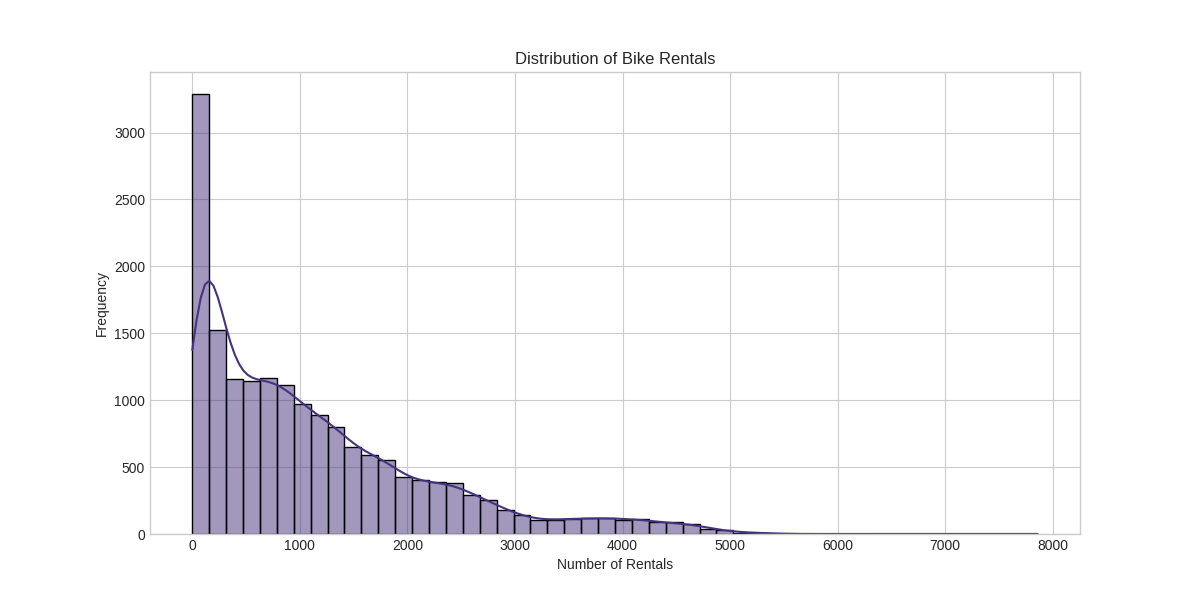
\includegraphics[width=1.0\textwidth]{eda_distribution.png}
\caption{Distribution of Bike Rentals}\label{o:2}
\end{figure}

\begin{figure}[ht!]
\centering
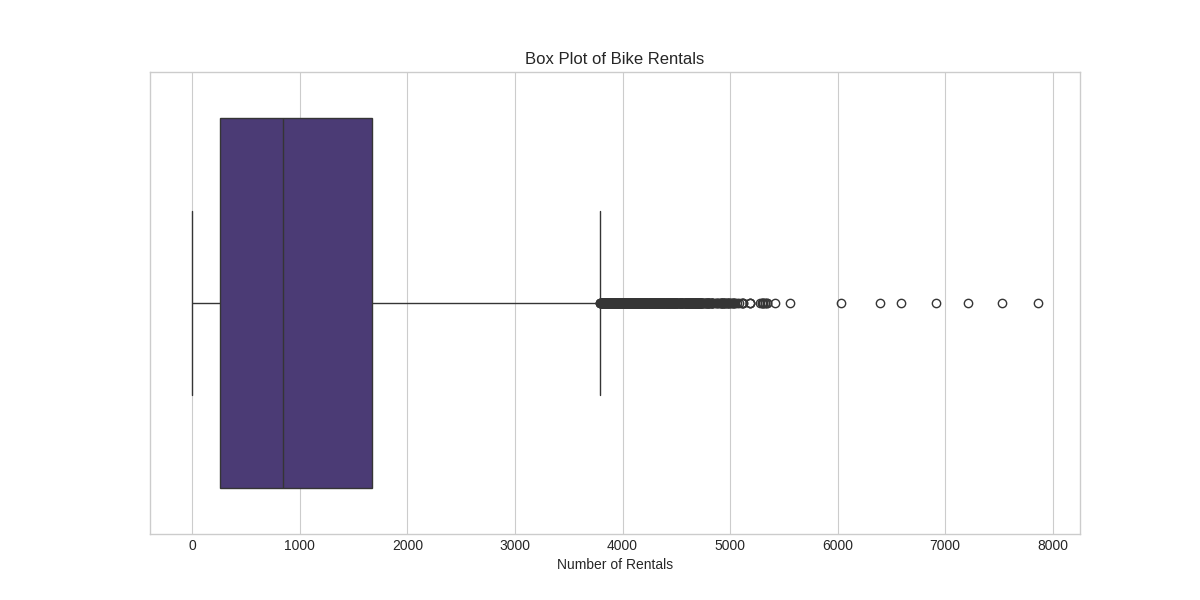
\includegraphics[width=1.0\textwidth]{eda_boxplot.png}
\caption{Box Plot of Bike Rentals}\label{o:2}
\end{figure}

\begin{figure}[ht!]
\centering
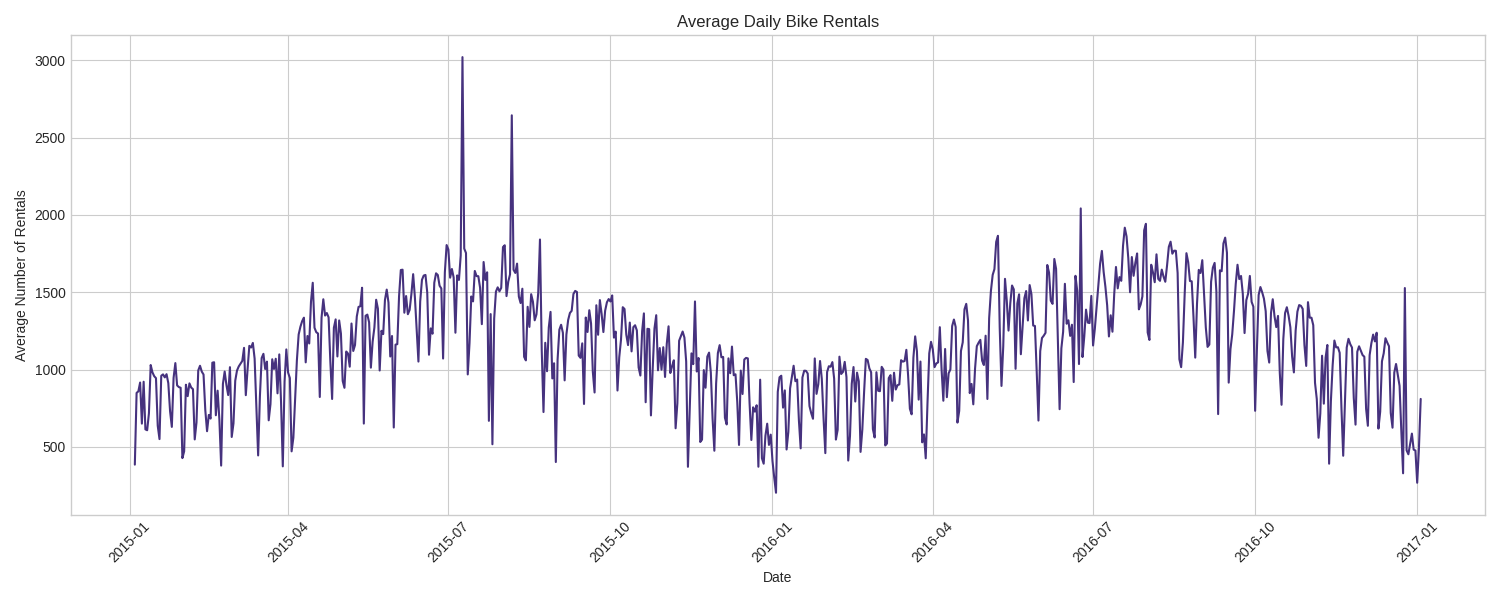
\includegraphics[width=1.0\textwidth]{eda_daily_rentals.png}
\caption{Average Daily Bike Rentals}\label{o:2}
\end{figure}

\newpage

\subsubsection{Predspracovanie a unifikácia dát}
Počas analýzy bolo identifikovaných niekoľko chýb a nekonzistentností v dátach, ktoré boli vyriešené predspracovaním a unifikáciou dát. Toto zahŕňalo:
\begin{itemize}
\item Riešenie chýbajúcich hodnôt a ich doplnenie alebo odstránenie
\item Normalizáciu a škálovanie dátových atribútov
\item Konverziu dátových typov a odstránenie redundantných dát
\end{itemize}

\subsubsection{Vytvorenie univerzálneho dátového načítača}
Pre zabezpečenie flexibility a všeobecnej použiteľnosti bol vytvorený univerzálny dátový načítač, ktorý umožňuje jednoducho načítať a spracovať ľubovoľný dataset bez nutnosti výraznej úpravy kódu. Tento načítač bol implementovaný v Python súbore pomocou knižníc pandas a numpy, čím je zabezpečená kompatibilita s rôznymi formátmi a štruktúrami dát.

% Implementácia flexibilného GRU modelu
\subsection{Implementácia flexibilného GRU modelu}
\label{sec:gru_model}
V rámci tejto práce bol implementovaný flexibilný GRU model, umožňujúci efektívne spracovanie sekvenčných dát a adaptáciu na rôzne typy úloh a dátových množín. Implementácia bola realizovaná pomocou PyTorch \cite{PyTorch}, pričom bola zabezpečená vysoká flexibilita modelu.

Kľúčové vlastnosti modelu zahŕňajú:
\begin{itemize}
\item Podpora jednej alebo viacerých vrstiev GRU.
\item Možnosť konfigurácie veľkostí skrytých vrstiev.
\item Použitie dropout vrstiev medzi GRU vrstvami na prevenciu pretrénovania.
\item Možnosť voľby jednosmernej alebo obojsmernej GRU architektúry.
\item Podpora návratu výstupov za celú sekvenciu alebo len z posledného kroku.
\end{itemize}

Implementovaný model je navrhnutý na základe jasne štruktúrovaného a dobre komentovaného Python kódu, čo umožňuje jednoduchú údržbu a budúce rozšírenia alebo modifikácie. Model bol navrhnutý s dôrazom na všeobecnú použiteľnosť a vysokú výpočtovú efektívnosť.

\newpage
% Metriky
\subsection{Realizácia metrík}
\label{sec:metrics}
Pre vyhodnotenie modelov boli implementované nasledujúce metriky:

\textbf{Mean Absolute Error (MAE)\label{mae}}: \[ MAE = \frac{1}{n} \sum_{i=1}^{n} \left| y_i - \hat{y}_i \right| \] Kde \( y_i \) je skutočná hodnota a \( \hat{y}_i \) je predikovaná hodnota.

\textbf{Mean Squared Error (MSE)\label{mse}}: \[ MSE = \frac{1}{n} \sum_{i=1}^{n} (y_i - \hat{y}_i)^2 \]

\textbf{Root Mean Squared Error (RMSE)\label{rmse}}: \[ RMSE = \sqrt{ \frac{1}{n} \sum_{i=1}^{n} (y_i - \hat{y}_i)^2 } \]

\textbf{R-squared (Coefficient of Determination)\label{r2}}: \[ R^2 = 1 - \frac{\sum_{i=1}^{n} (y_i - \hat{y}_i)^2}{\sum_{i=1}^{n} (y_i - \bar{y})^2} \] Kde \( \bar{y} \) je priemerná hodnota skutočných výstupov.

\textbf{Mean Absolute Percentage Error (MAPE)\label{mape}}: \[ MAPE = \frac{100\%}{n} \sum_{i=1}^{n} \left| \frac{y_i - \hat{y}_i}{y_i} \right| \]

\textbf{Symmetric Mean Absolute Percentage Error (sMAPE)\label{smape}}: \[ SMAPE = \frac{100\%}{n} \sum_{i=1}^{n} \frac{ \left| y_i - \hat{y}_i \right| }{ \left( |y_i| + |\hat{y}_i| \right) / 2 } \]

\textbf{Explained Variance (EV)\label{ev}}: \[ EV = 1 - \frac{\mathrm{Var}(y - \hat{y})}{\mathrm{Var}(y)} \] Kde \( \mathrm{Var}(\cdot) \) označuje štatistickú varianciu.

\textbf{Peak Error (Maximum Absolute Error)\label{pe}}: \[ PE = \max_{i} \left| y_i - \hat{y}_i \right| \]

Tieto metriky boli implementované pomocou knižníc numpy a pandas, čo zabezpečuje transparentnosť a kontrolovateľnosť procesu výpočtov.

% Experimenty
\subsection{Priebeh experimentov}

Táto kapitola opisuje proces vykonávania experimentov, ktoré zahŕňali hľadanie a optimalizáciu hyperparametrov pre GRU model pomocou metód Random Search, Bayesian Search a následne Grid Search. Cieľom bolo identifikovať najlepšiu kombináciu hyperparametrov pre čo najvyššiu výkonnosť modelu.

\subsubsection{Počiatočná sieť hyperparametrov}

Pre experimenty bola vytvorená nasledujúca počiatočná sieť hyperparametrov:

\begin{table}[ht!]
\centering
\caption{Počiatočná sieť hyperparametrov}\label{t:hyperparams}
\medskip
\small
\begin{tabular}{||l||l||}
\hhline{|t:==:t|}
\multicolumn{1}{||c||}{\textbf{Hyperparameter}} & \multicolumn{1}{c||}{\textbf{Hodnoty}} \\
\hhline{|:==:|}
Hidden size & 32, 64, 128, 256, 512 \\
\hline
Počet vrstiev & 1, 2, 3, 4, 5 \\
\hline
Dropout & 0.0, 0.1, 0.2, 0.3, 0.4, 0.5 \\
\hline
Learning rate & 0.01, 0.001, 0.0001, 0.00001 \\
\hline
Weight decay & 0.0, 0.0001, 0.001, 0.00001 \\
\hline
Bidirectional & False, True \\
\hline
Early stopping patience & 5, 10, 15 \\
\hline
Learning rate factor & 0.5, 0.25, 0.1 \\
\hline
Learning rate patience & 5, 10 \\
\hhline{|b:==:b|}
\end{tabular}
\end{table}
Táto široká sieť parametrov umožnila dôkladné preskúmanie možností a určenie, ktoré hyperparametre majú najvýznamnejší vplyv na výkonnosť modelu. Rozmanitosť nastavení bola zvolená zámerne, aby boli pokryté extrémne aj stredné hodnoty hyperparametrov a ich interakcie.

Podrobný log výsledkov je verejne dostupný v prislušnom notebooku \texttt{experiments.ipynb} na GitHub \cite{GitHub} repozitári projektu.

\newpage

\subsubsection{Výsledky Random Search}
\label{sec:random_search}
Random Search dosiahol nasledovné najlepšie výsledky:

\begin{table}[ht!]
\centering
\caption{Výsledky Random Search}\label{t:random_search}
\medskip
\small
\begin{tabular}{||l||l||}
\hhline{|t:==:t|}
\multicolumn{1}{||c||}{\textbf{Hyperparameter}} & \multicolumn{1}{c||}{\textbf{Najlepšia hodnota}} \\
\hhline{|:==:|}
Validation RMSE & 0.054382 \\
\hline
Hidden size & 512 \\
\hline
Počet vrstiev & 1 \\
\hline
Dropout & 0.0 \\
\hline
Learning rate & 0.0001 \\
\hline
Weight decay & 0.0001 \\
\hline
Bidirectional & True \\
\hline
Early stopping patience & 15 \\
\hline
Learning rate factor & 0.5 \\
\hline
Learning rate patience & 10 \\
\hhline{|b:==:b|}
\end{tabular}
\end{table}

Random Search umožnil efektívne preskúmať náhodne zvolené kombinácie, čím sa zvýšila pravdepodobnosť nájdenia dobre fungujúcich kombinácií, ktoré by grid search \cite{GridSearch} mohol prehliadnuť. Táto metóda poskytla dobré východiskové body pre ďalšie optimalizačné kroky.

\newpage

\subsubsection{Výsledky Bayesian Search}
\label{sec:bayesian_search}
Bayesian Search dosiahol mierne lepší výsledok:

\begin{table}[ht!]
\centering
\caption{Výsledky Bayesian Search}\label{t:bayesian_search}
\medskip
\small
\begin{tabular}{||l||l||}
\hhline{|t:==:t|}
\multicolumn{1}{||c||}{\textbf{Hyperparameter}} & \multicolumn{1}{c||}{\textbf{Najlepšia hodnota}} \\
\hhline{|:==:|}
Validation RMSE & 0.054269 \\
\hline
Hidden size & 128 \\
\hline
Počet vrstiev & 2 \\
\hline
Dropout & 0.1 \\
\hline
Learning rate & 0.01 \\
\hline
Weight decay & 0.0 \\
\hline
Bidirectional & True \\
\hline
Early stopping patience & 15 \\
\hline
Learning rate factor & 0.1 \\
\hline
Learning rate patience & 10 \\
\hhline{|b:==:b|}
\end{tabular}
\end{table}

Bayesian Search bol efektívnejší v hľadaní optimálnych hyperparametrov vďaka svojmu adaptívnemu prístupu, ktorý využíva predchádzajúce výsledky na inteligentnejšie nasmerovanie ďalších experimentov. Výsledkom bola rýchlejšia konvergencia k optimálnym riešeniam.

\newpage

\subsubsection{Analýza najlepších sád hyperparametrov}
Z kombinovaných výsledkov Random a Bayesian Search boli vybrané tri najlepšie sady hyperparametrov:

\begin{table}[ht!]
\centering
\caption{Najlepšie sady hyperparametrov z Random a Bayesian Search}\label{t:best_hyperparams}
\medskip
\small
\begin{tabular}{||c||c|c|c||}
\hhline{|t:====:t|}
\multicolumn{1}{||c||}{\textbf{Hyperparameter}} & \multicolumn{1}{c|}{\textbf{Sada 1}} & \multicolumn{1}{c|}{\textbf{Sada 2}} & \multicolumn{1}{c||}{\textbf{Sada 3}} \\
\hhline{|:====:|}
Hidden size & 128 & 512 & 64 \\
\hline
Počet vrstiev & 2 & 1 & 1 \\
\hline
Dropout & 0.1 & 0.0 & 0.0 \\
\hline
Learning rate & 0.01 & 0.0001 & 0.01 \\
\hline
Weight decay & 0.0 & 0.0001 & 1e-05 \\
\hline
Bidirectional & True & True & False \\
\hline
Early stopping patience & 15 & 15 & 10 \\
\hline
Learning rate factor & 0.1 & 0.5 & 0.5 \\
\hline
Learning rate patience & 10 & 10 & 10 \\
\hline
RMSE & 0.054269 & 0.054382 & 0.054632 \\
\hhline{|b:====:b|}
\end{tabular}
\end{table}

Tieto tri najlepšie kombinácie hyperparametrov boli vybrané na základe dosiahnutých hodnôt RMSE \ref{rmse} a slúžili ako východiskový bod pre detailnejšiu optimalizáciu pomocou Grid Search \ref{sec:grid_search}. Ich výber reflektuje rôznorodosť úspešných konfigurácií, čo umožňuje hlbšie pochopenie ich vplyvu na model.

\newpage

\subsubsection{Grid Search optimalizácia}
\label{sec:grid_search}
Z dôvodu obmedzených výpočtových kapacít pre spracovanie veľkého množstva kombinácií sme na základe predchádzajúcej analýzy \ref{t:best_hyperparams} vytvorili finálnu optimalizačnú sieť pre Grid Search:

\begin{table}[ht!]
\centering
\caption{Grid Search optimalizačná sieť}\label{t:grid_search}
\medskip
\small
\begin{tabular}{||l||c||}
\hhline{|t:==:t|}
\multicolumn{1}{||c||}{\textbf{Hyperparameter}} & \multicolumn{1}{c||}{\textbf{Hodnoty}} \\
\hhline{|:==:|}
Hidden size & 64, 128, 256 \\
\hline
Počet vrstiev & 2, 3 \\
\hline
Dropout & 0.0, 0.3 \\
\hline
Learning rate & 0.001, 0.0001, 0.00001 \\
\hline
Weight decay & 0.0001, 0.00001 \\
\hline
Bidirectional & True \\
\hline
Early stopping patience & 10 \\
\hline
Learning rate factor & 0.25 \\
\hline
Learning rate patience & 5, 10 \\
\hhline{|b:==:b|}
\end{tabular}
\end{table}

Táto zúžená optimalizačná sieť bola navrhnutá na základe predchádzajúcich výsledkov, aby sa minimalizoval počet testovaných kombinácií a zároveň sa maximalizovala efektivita výpočtových zdrojov. Grid Search týmto umožnil dôkladné preskúmanie najperspektívnejších oblastí parametrového priestoru.

\newpage

Po vykonaní viac ako 500 rôznych kombinácií Grid Search bola nájdená najlepšia sada parametrov:

\begin{table}[ht!]
\centering
\caption{Najlepšie hyperparametre z Grid Search}\label{t:best_grid_search}
\medskip
\small
\begin{tabular}{||l||c||}
\hhline{|t:==:t|}
\multicolumn{1}{||c||}{\textbf{Hyperparameter}} & \multicolumn{1}{c||}{\textbf{Najlepšia hodnota}} \\
\hhline{|:==:|}
Hidden size & 64 \\
\hline
Počet vrstiev & 2 \\
\hline
Dropout & 0.0 \\
\hline
Learning rate & 0.01 \\
\hline
Weight decay & 1e-05 \\
\hline
Bidirectional & False \\
\hline
Early stopping patience & 15 \\
\hline
Learning rate factor & 0.1 \\
\hline
Learning rate patience & 10 \\
\hline
Najlepšie RMSE & 0.052874 \\
\hhline{|b:==:b|}
\end{tabular}
\end{table}

Táto optimálna sada parametrov bola následne použitá na tréning finálnej verzie modelu, čím bol úspešne ukončený optimalizačný proces.

% Vizualizácia výsledkov
\section{Analýza a vizualizácia výsledkov}

Táto kapitola sa venuje detailnej analýze a interpretácii výsledkov získaných počas optimalizácie hyperparametrov a tréningu modelu pomocou metód Random Search \ref{sec:random_search}, Bayesian Search \ref{sec:bayesian_search}, Grid Search \ref{sec:grid_search} a následnej finálnej optimalizácie modelu.

\subsection{Vizualizácia výsledkov Random Search}

Random Search umožnil rýchle preskúmanie veľkého priestoru hyperparametrov. Výsledky z Random Search boli analyzované pomocou viacerých grafických vizualizácií, ktoré poskytujú prehľad o výkonnosti modelu v závislosti od použitých hyperparametrov.

\subsubsection{Progres vyhľadávania}
Graf progresu vyhľadávania ukazuje, ako sa menila najlepšia hodnota RMSE počas jednotlivých pokusov. Tento graf poukazuje na stabilizáciu výsledkov okolo najlepšej hodnoty po niekoľkých počiatočných pokusoch.

\begin{figure}[ht!]
\centering
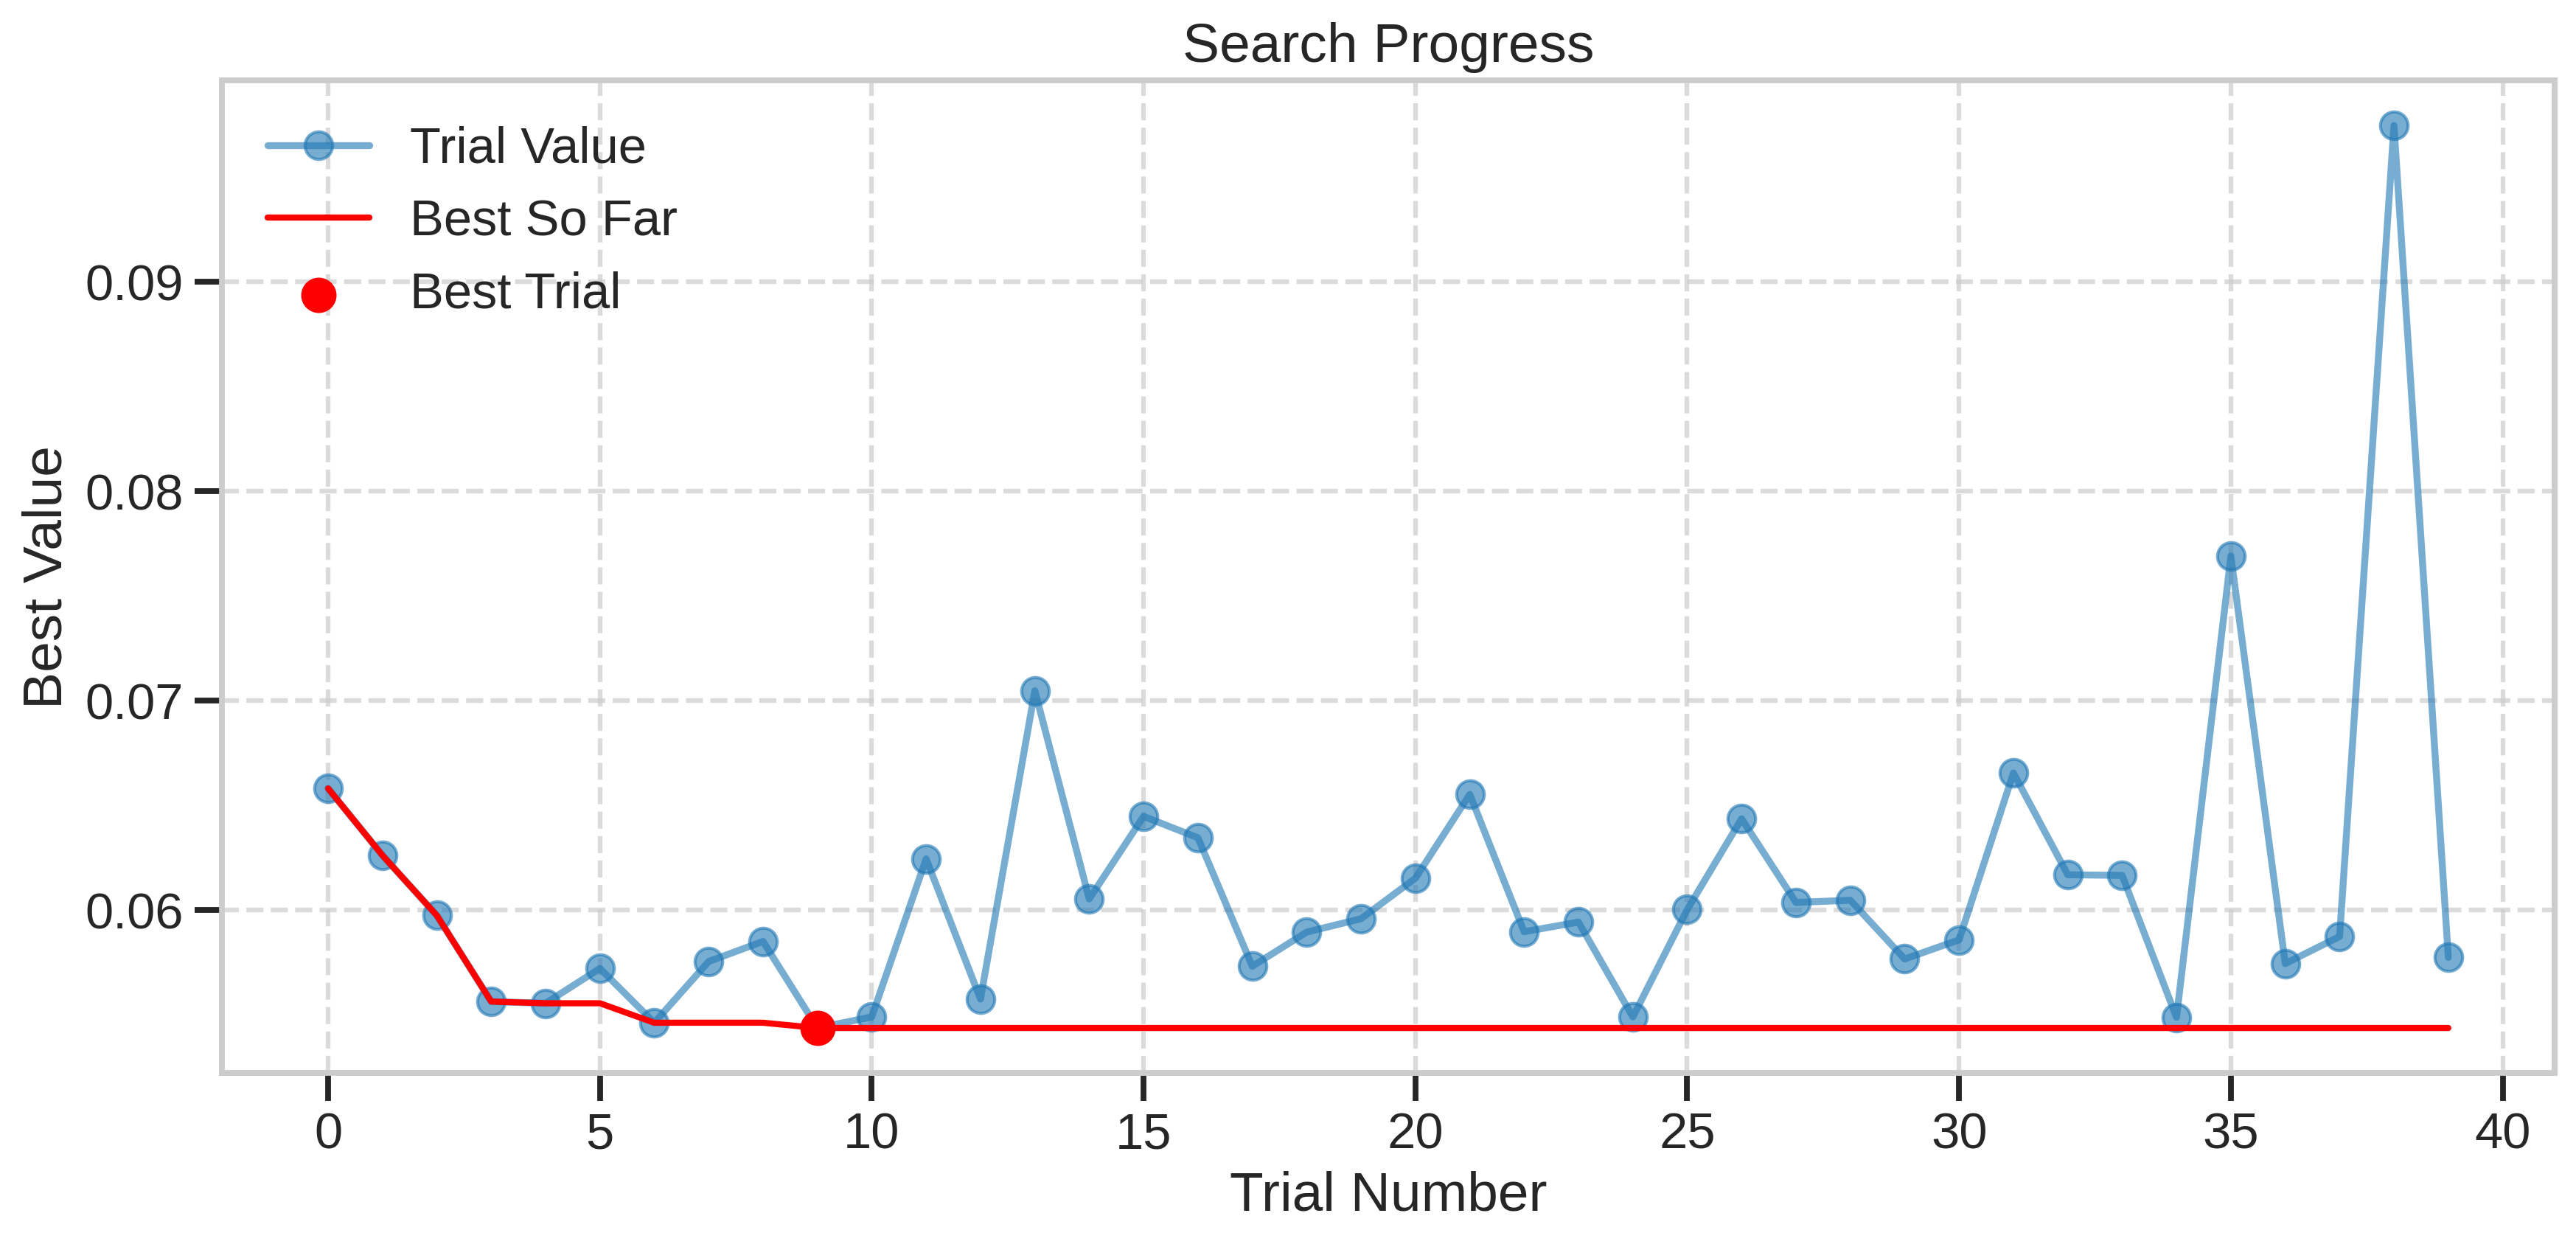
\includegraphics[width=\textwidth]{random_search_search_progress.png}
\caption{Progres vyhľadávania}
\label{fig:random_search_search_progress}
\end{figure}
Analýza grafu odhaľuje, že v počiatočnej fáze experimentov bolo pozorované lineárne klesanie hodnoty RMSE, čo indikuje systematické zlepšovanie výkonnosti modelu. Avšak po aproximatívne 10 experimentoch dochádza k výraznej volatilite v hodnotách RMSE. Pozoruhodné je, že optimálna hodnota RMSE bola dosiahnutá už pri deviatom experimente. Následná vysoká volatilita hodnôt naznačuje, že ďalšie testované kombinácie hyperparametrov boli menej efektívne, čo potvrdzuje, že algoritmus random search úspešne identifikoval oblasť optimálneho nastavenia v relatívne skorej fáze experimentovania.

\newpage

\subsubsection{Vzťah medzi epochami a stratou (Loss)}
Graf Epochs vs Loss zobrazuje priebeh trénovacej a validačnej chyby počas tréningových epoch. Tento graf nám umožňuje sledovať, ako rýchlo a efektívne model konverguje.

\begin{figure}[ht!]
\centering
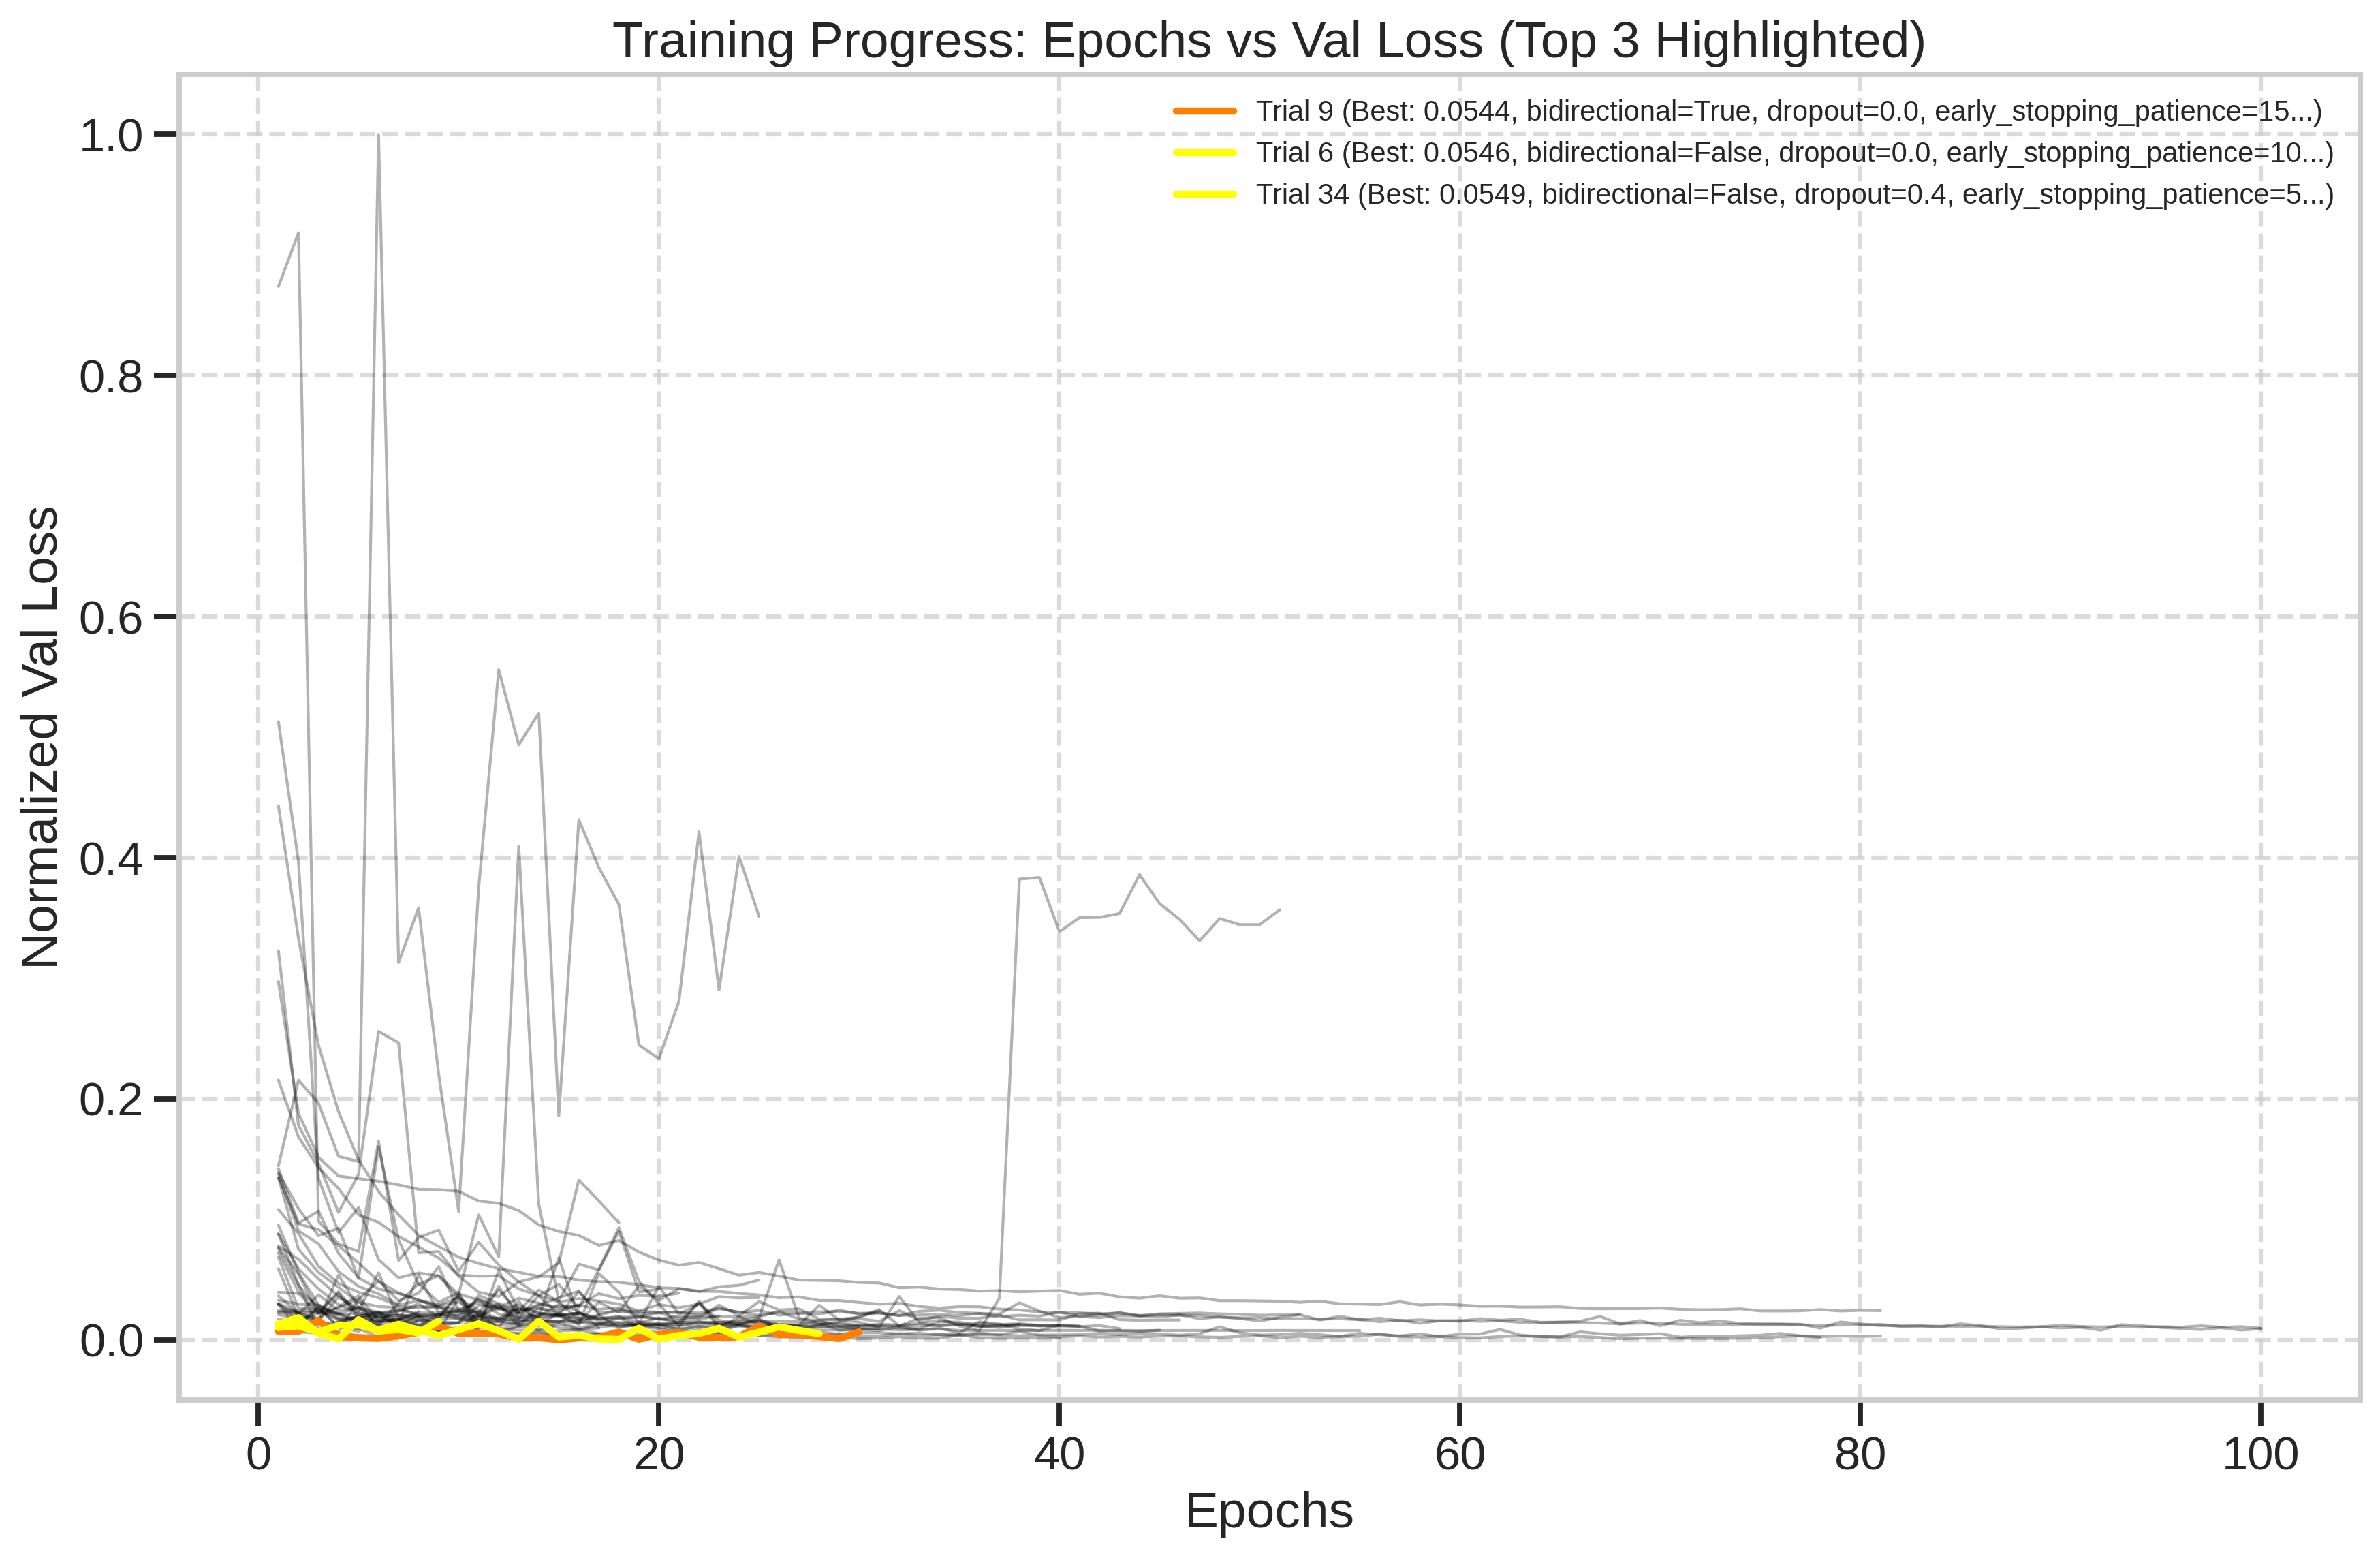
\includegraphics[width=\textwidth]{random_search_epochs_vs_loss.png}
\caption{Epochs vs Loss}
\label{fig:random_search_epochs_vs_loss}
\end{figure}

Pozorujeme významnú variabilitu v procesoch učenia, ako aj vysokú volatilitu medzi rôznymi kombináciami hyperparametrov. Najmenej efektívne kombinácie vykazujú extrémnu volatilitu a vo väčšine prípadov vysokú hodnotu funkcie straty. Väčšina kombinácií demonštruje pomalú schopnosť učenia, pri ktorej funkcia straty klesá lineárne, čo nie je optimálne z hľadiska efektivity. Najlepšie kombinácie vykazujú nízku hodnotu funkcie straty, rýchlo ukončujú proces učenia na zabránenie pretrénovaniu, pričom rozdiel v hodnotách funkcie straty sa prejavuje až na treťom desatinnom mieste.

\newpage

\subsubsection{Vplyv veľkosti skrytých vrstiev (Hidden size)}
Analýza vplyvu veľkosti skrytej vrstvy ukazuje, ako tento parameter ovplyvňuje celkovú chybu modelu. Z grafu je možné vidieť, že optimálne výsledky sa pohybovali okolo stredných až vyšších hodnôt veľkosti skrytých vrstiev.

\begin{figure}[ht!]
\centering
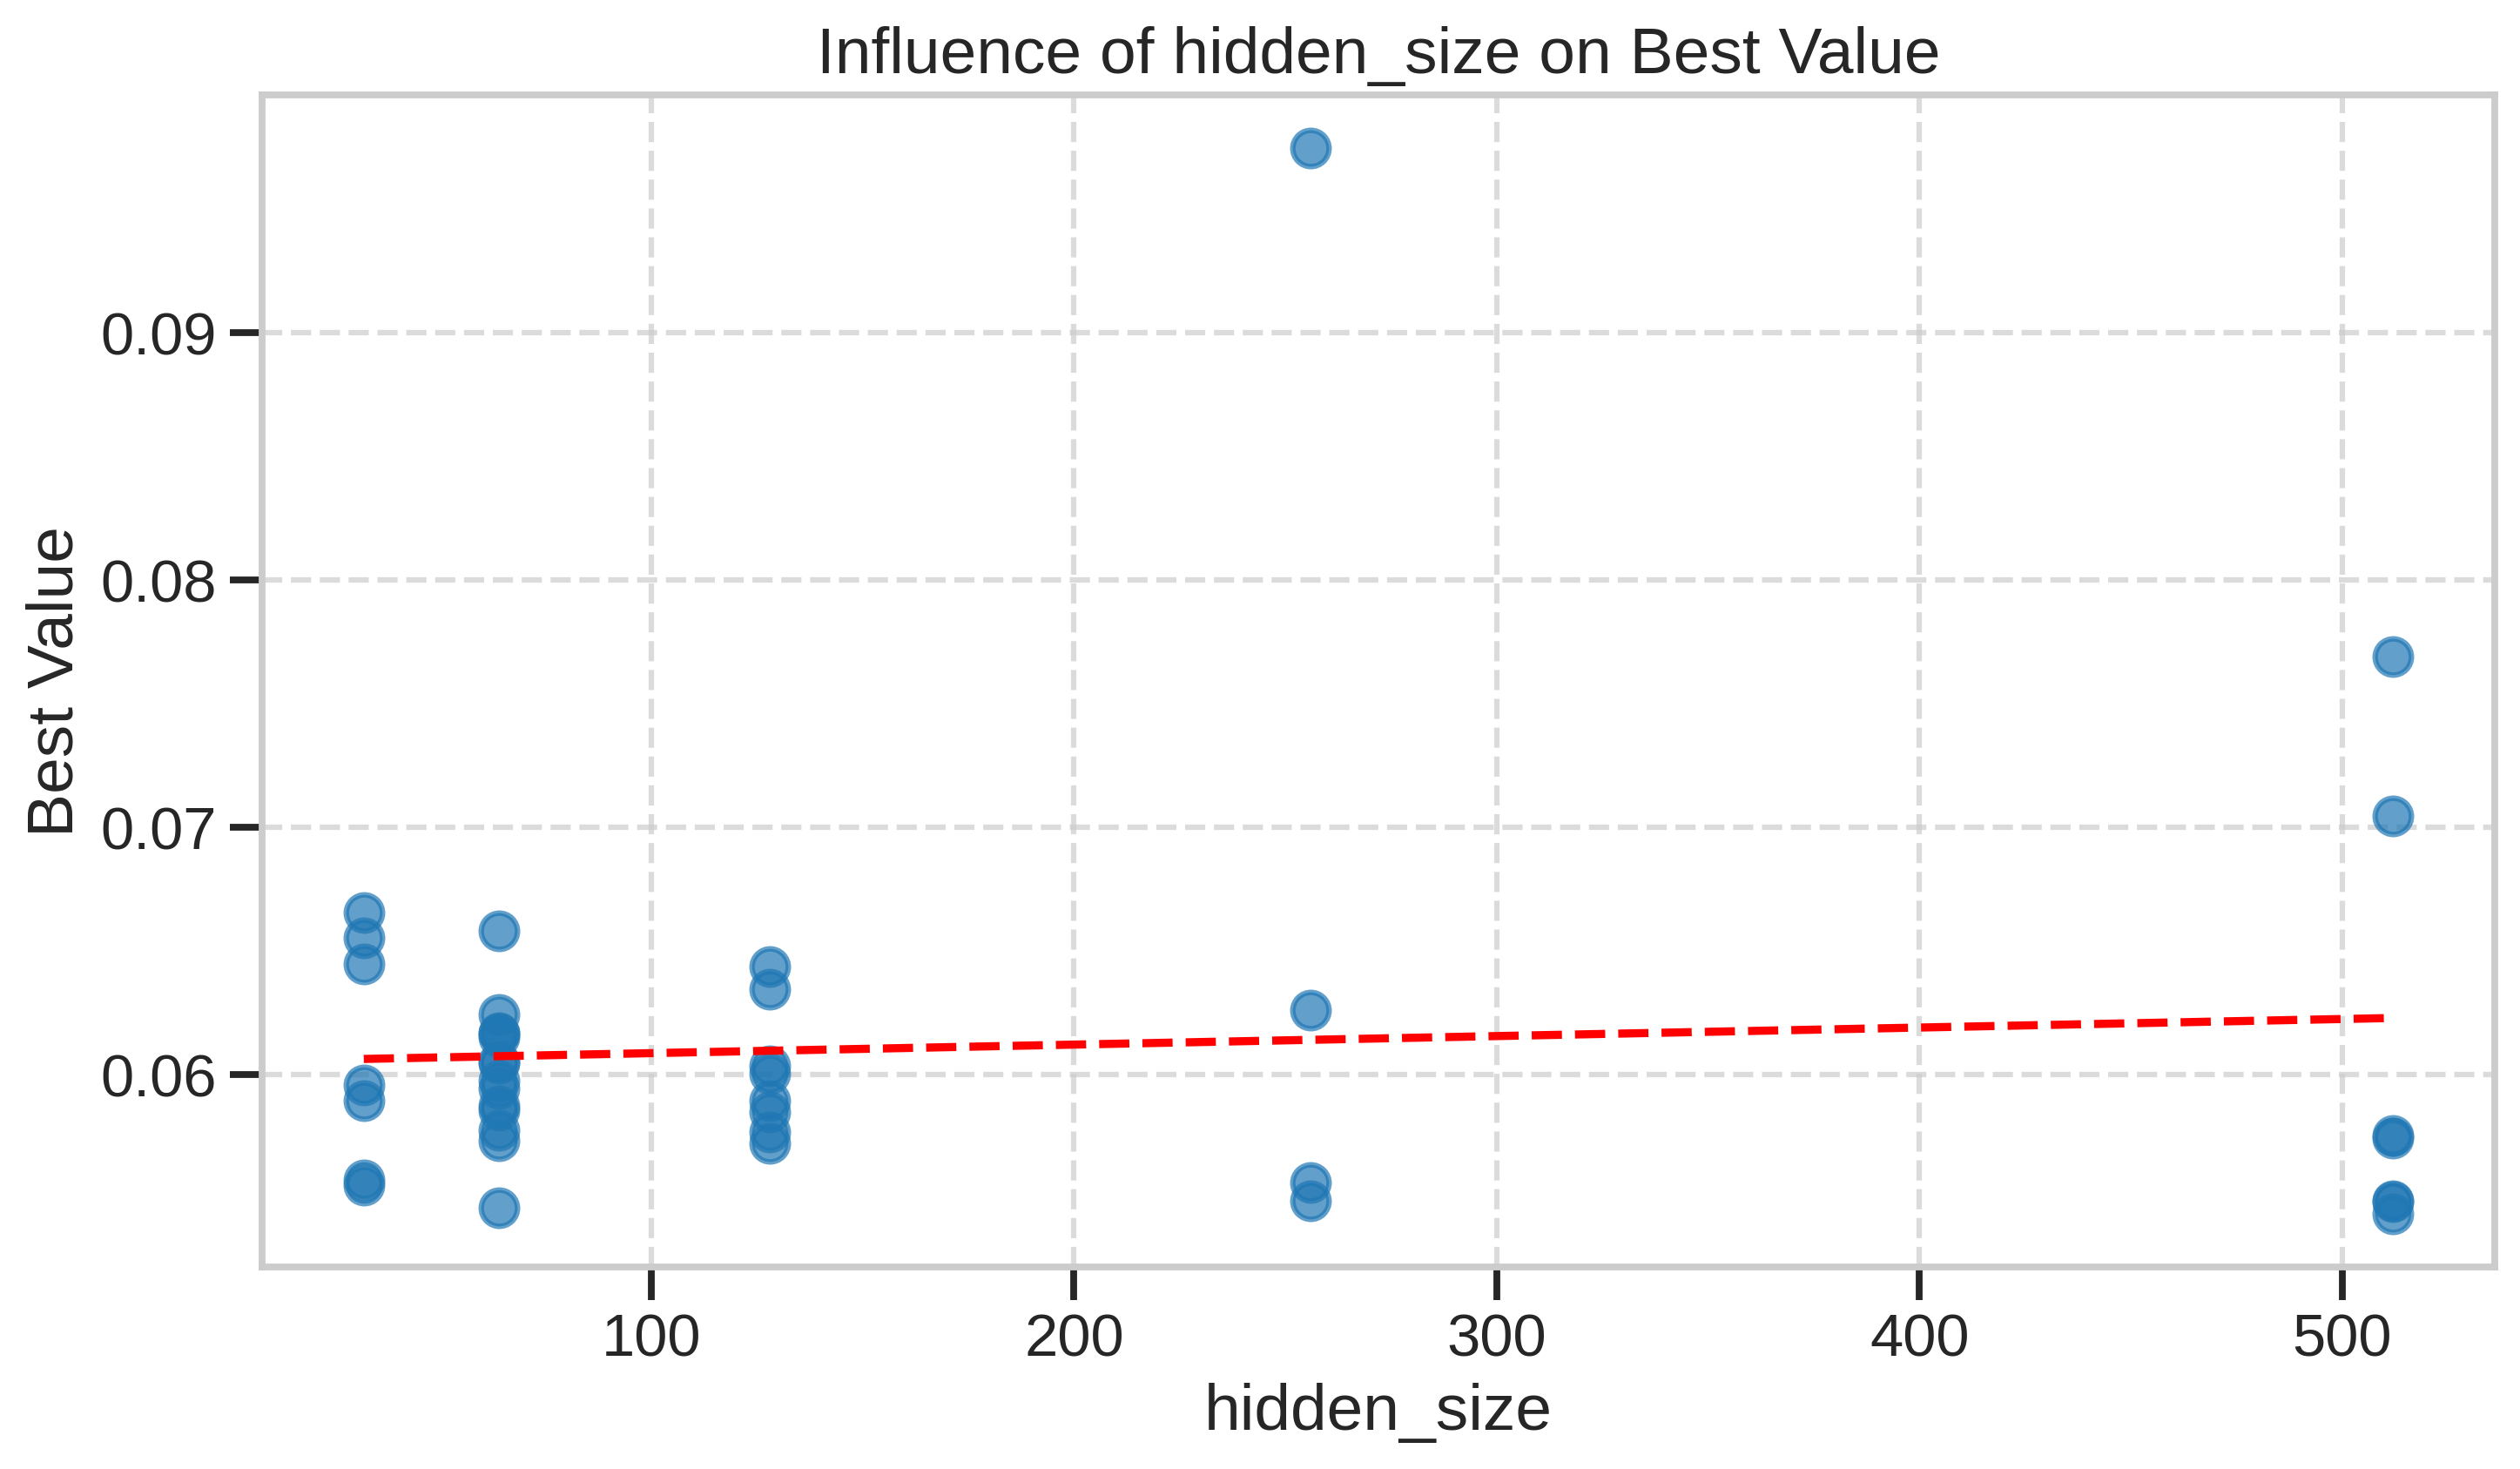
\includegraphics[width=\textwidth]{random_search_hidden_size_influence.png}
\caption{Hidden size influence}
\label{fig:random_search_hidden_size_influence}
\end{figure}

Vplyv veľkosti skrytých blokov sa vzájomne výrazne nelíši, s výnimkou rýchlosti učenia. Čím väčšia je veľkosť skrytých blokov, tým dlhšie trvá tréning modelu. Napriek hlbšej architektúre výsledky ukazujú, že menšia veľkosť skrytých blokov vykazuje menší rozptyl a stabilnejšie výsledky. Zároveň takmer každá veľkosť skrytých blokov má kombinácie, ktoré demonštrujú takmer nerozlíšiteľné hodnoty funkcie straty.

\newpage

\subsubsection{Krivky učenia (Learning curves)}
Krivky učenia demonštrujú vývoj chyby (loss) a metriky MAE počas tréningu a validácie. Táto analýza poskytuje pohľad na schopnosť modelu generalizovať na nové dáta.

\begin{figure}[ht!]
\centering
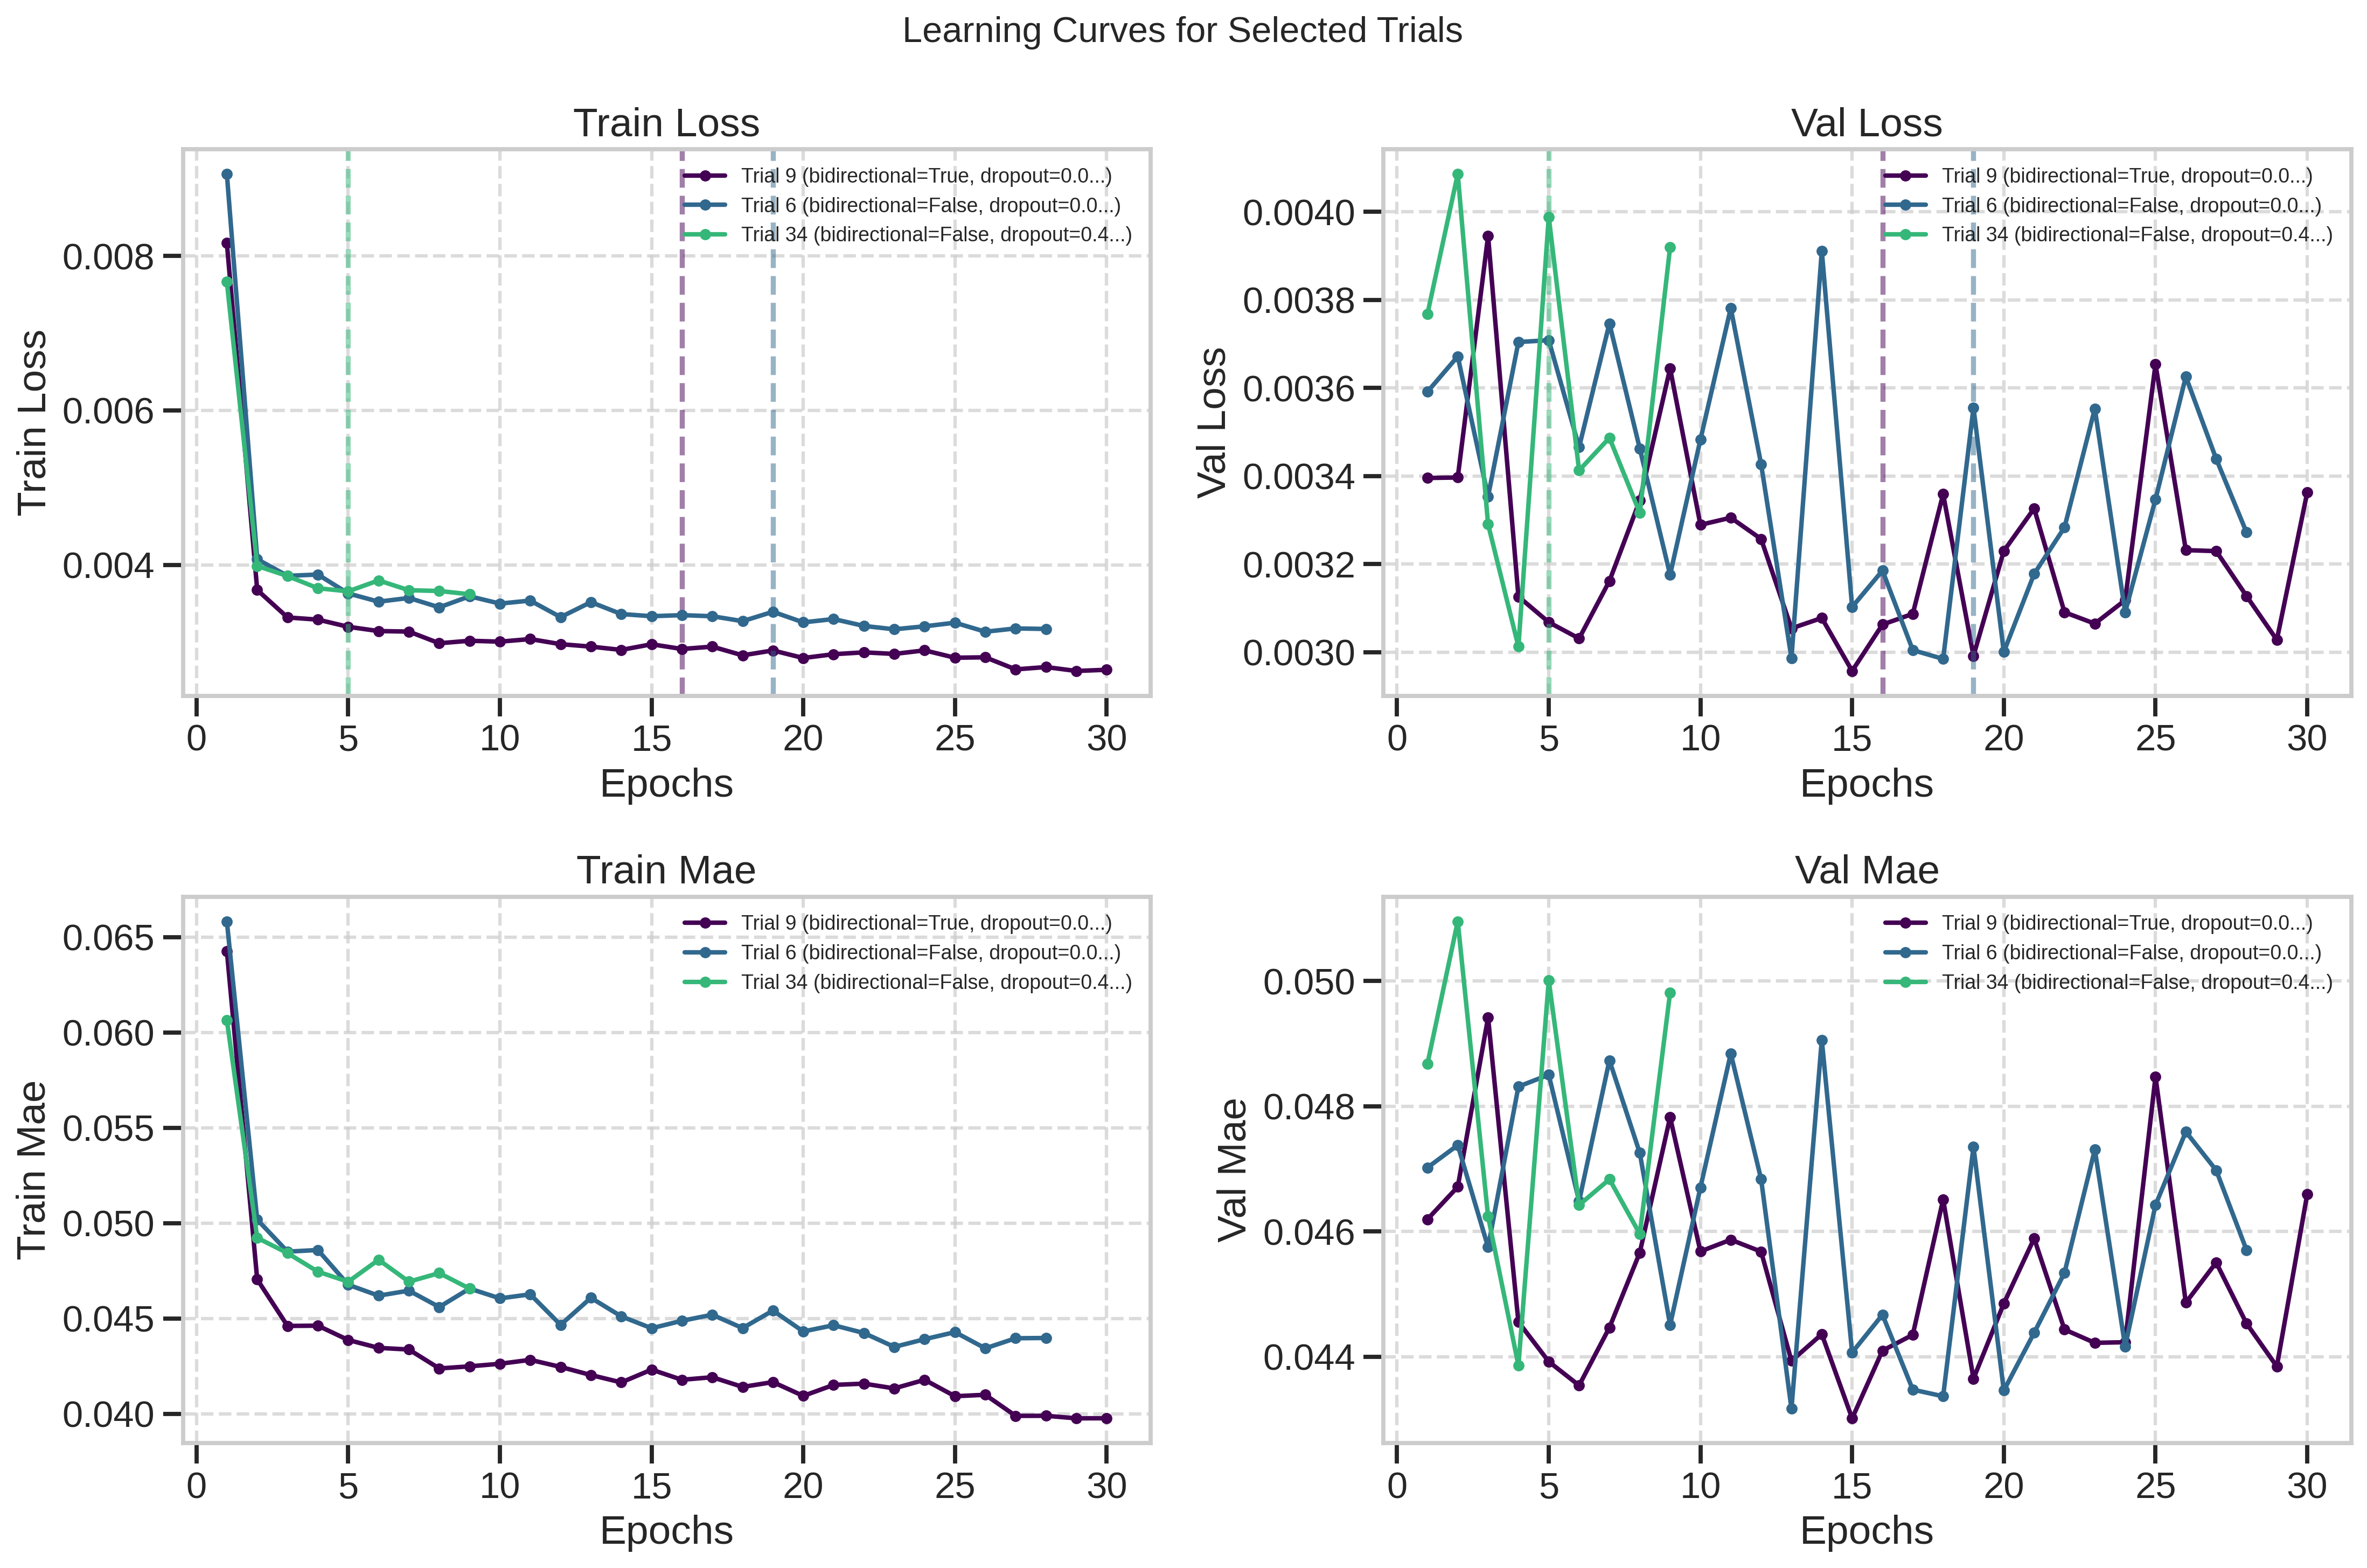
\includegraphics[width=\textwidth]{random_search_learning_curves.png}
\caption{Learning curves}
\label{fig:random_search_learning_curves}
\end{figure}

Pozorujeme očakávané lineárne zníženie funkcie straty počas trénovania pre 3 najlepšie modely. Počas validačnej fázy metriky vykazujú porovnateľný pokles, avšak s vyššou volatilitou. Napriek tomu každý z modelov dosahuje presvedčivé pozitívne výsledky. Vysoká volatilita bez výrazného zníženia funkcie straty môže signalizovať pretrénovanie modelov.

\newpage

\subsubsection{Korelácia medzi parametrami a výkonom}
Graf korelácie medzi parametrami a výkonom znázorňuje, ako jednotlivé parametre ovplyvňujú výslednú hodnotu RMSE. Z tohto grafu je možné identifikovať parametre, ktoré majú najväčší vplyv na výkon modelu.

\begin{figure}[ht!]
\centering
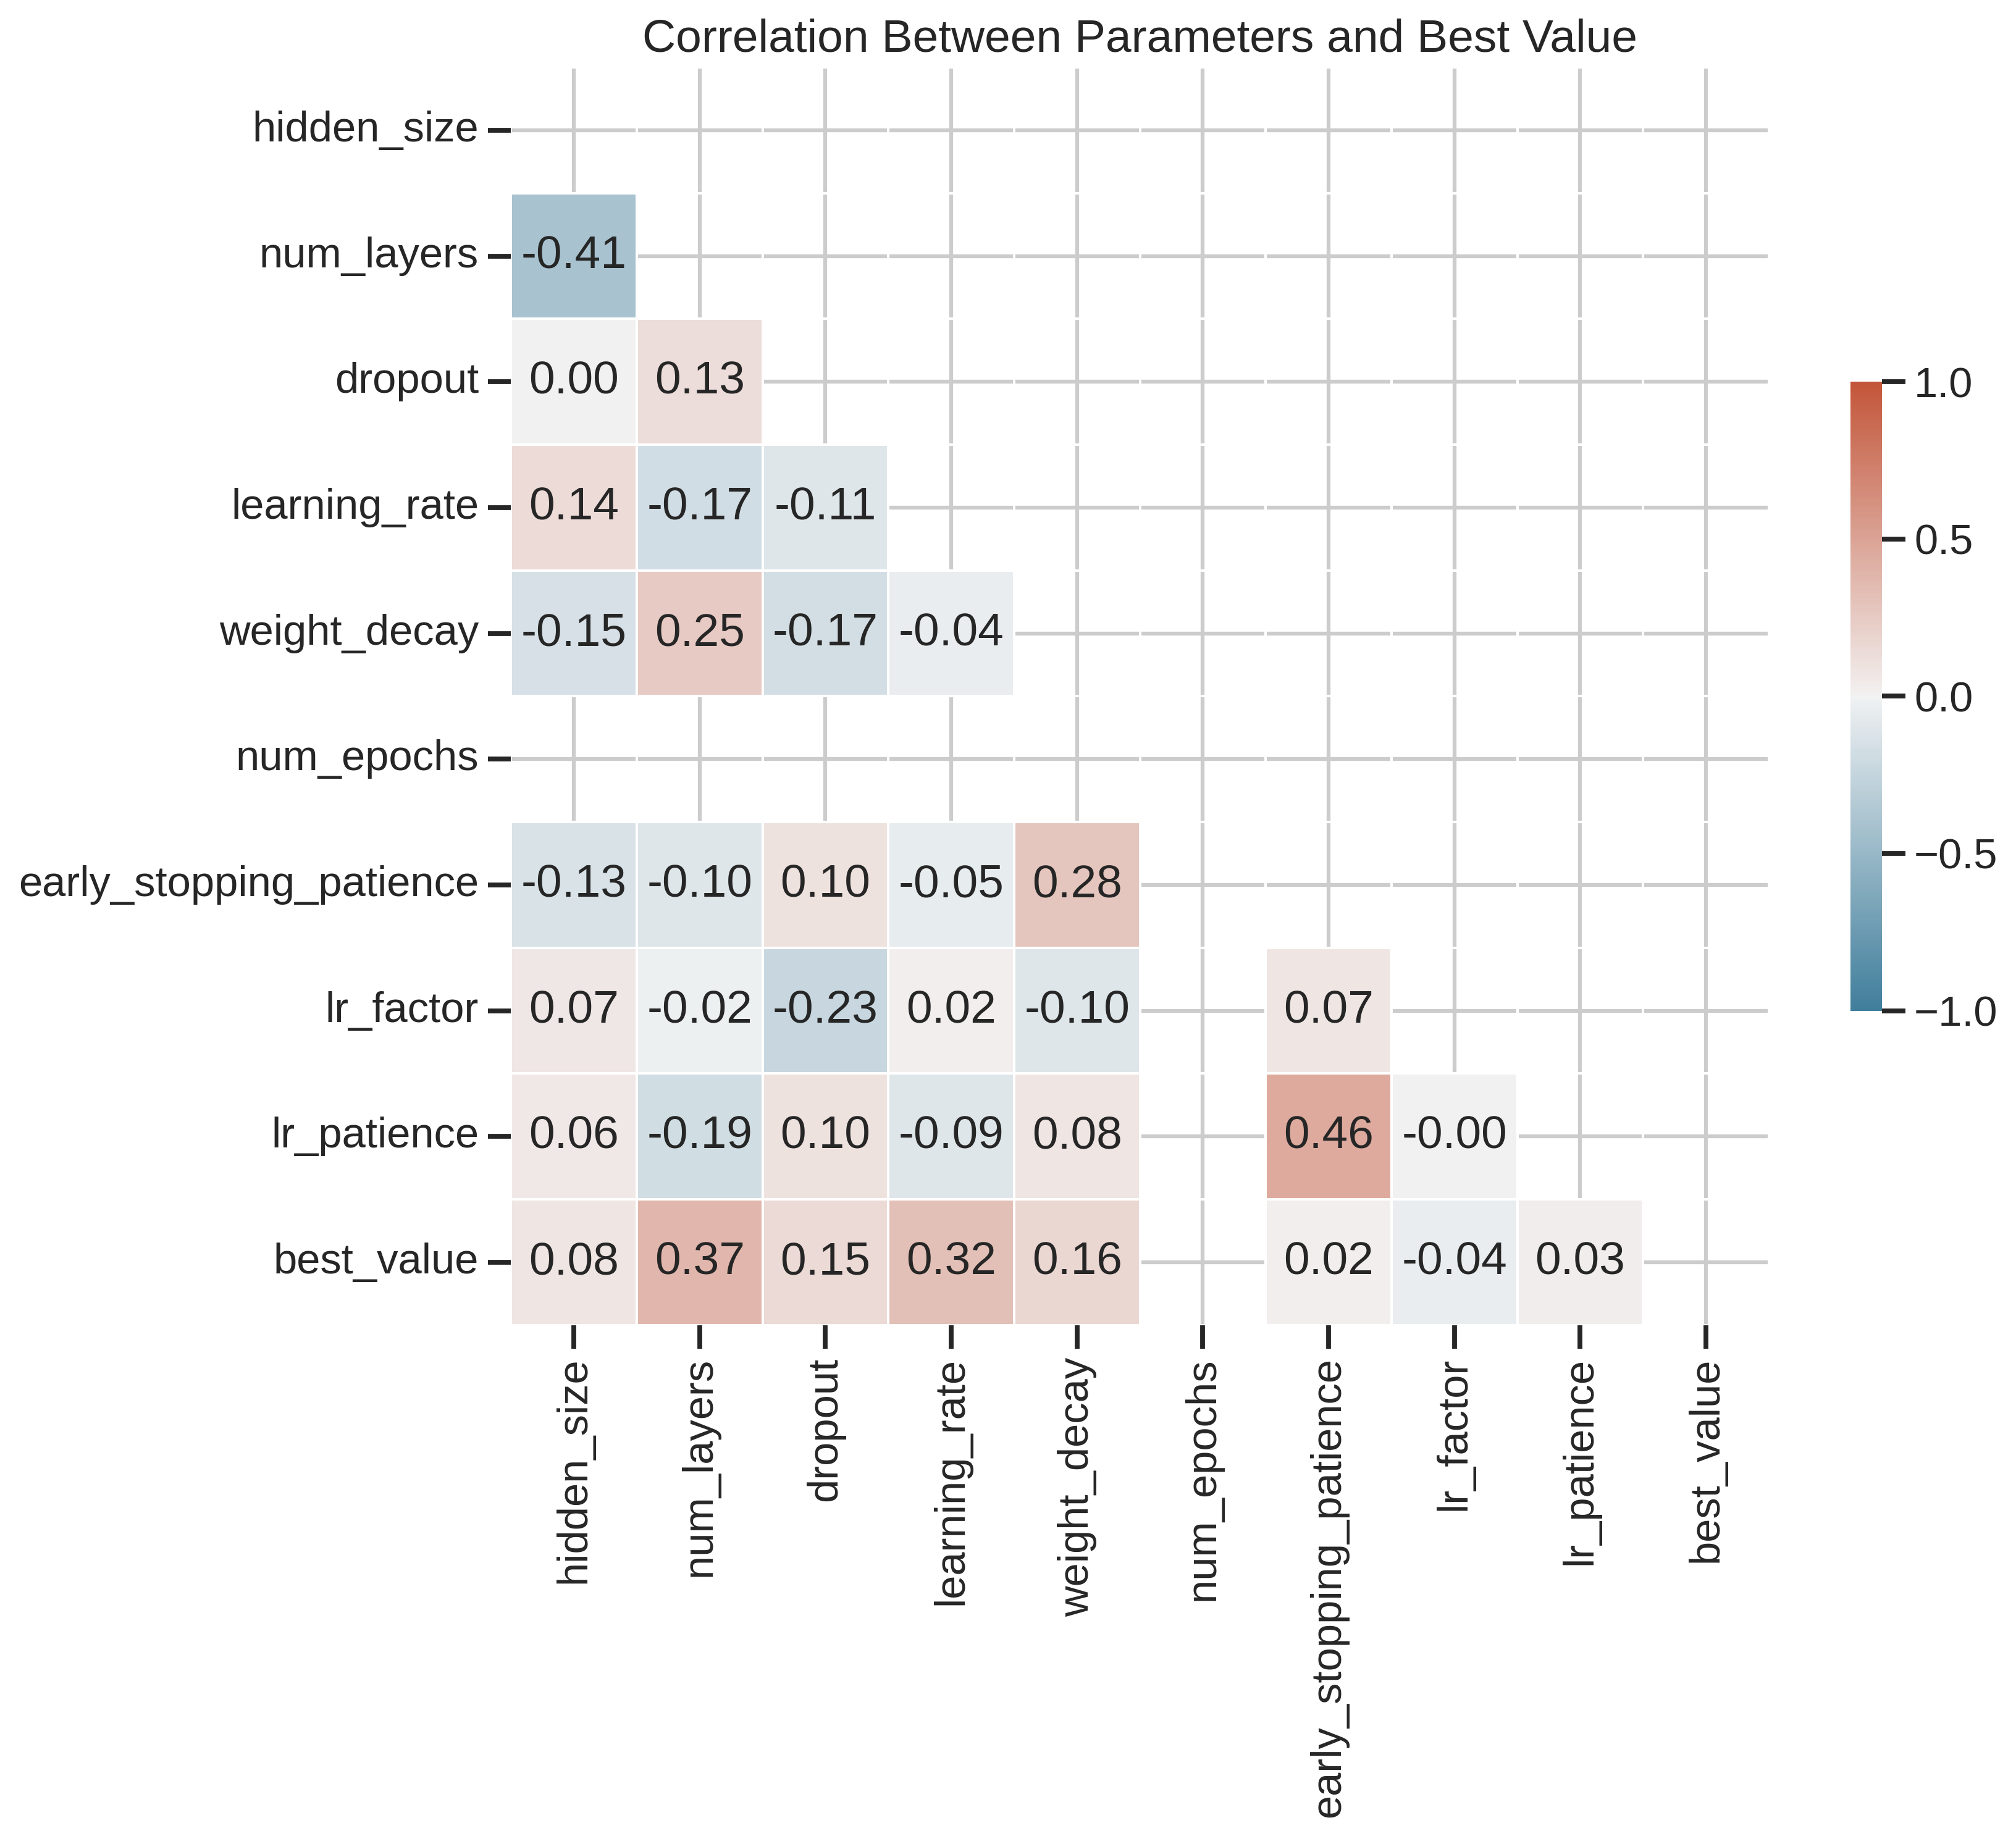
\includegraphics[width=0.9\textwidth]{random_search_parameter_correlation.png}
\caption{Parameter correlation}
\label{fig:random_search_parameter_correlation}
\end{figure}

Korelačná matica nám názorne demonštruje, že na výsledky najväčším spôsobom vplývali nasledujúce parametre: počet skrytých vrstiev a počiatočná hodnota learning rate. Zároveň pozorujeme priamy vzájomný vplyv early stopping patience na lr patience, čo môže signalizovať, že learning rate sa nestihol znížiť pre ďalšie trénovanie modelu, kvôli čomu boli tieto kombinácie označené ako neefektívne z dôvodu nedostatočného tréningu.

\subsection{Vizualizácia výsledkov Bayesian Search}

Bayesian Search je efektívna optimalizačná metóda, ktorá umožňuje inteligentné hľadanie hyperparametrov s využitím informácií z predchádzajúcich pokusov. Táto metóda rýchlo konvergovala k optimálnym výsledkom, čo potvrdzuje aj graf progresu vyhľadávania.

\subsubsection{Progres vyhľadávania (Search Progress)}
Graf progresu vyhľadávania ukazuje, ako sa menila najlepšia hodnota RMSE počas jednotlivých pokusov. Tento graf poukazuje na stabilizáciu výsledkov okolo najlepšej hodnoty po niekoľkých počiatočných pokusoch. 

\begin{figure}[ht!]
\centering
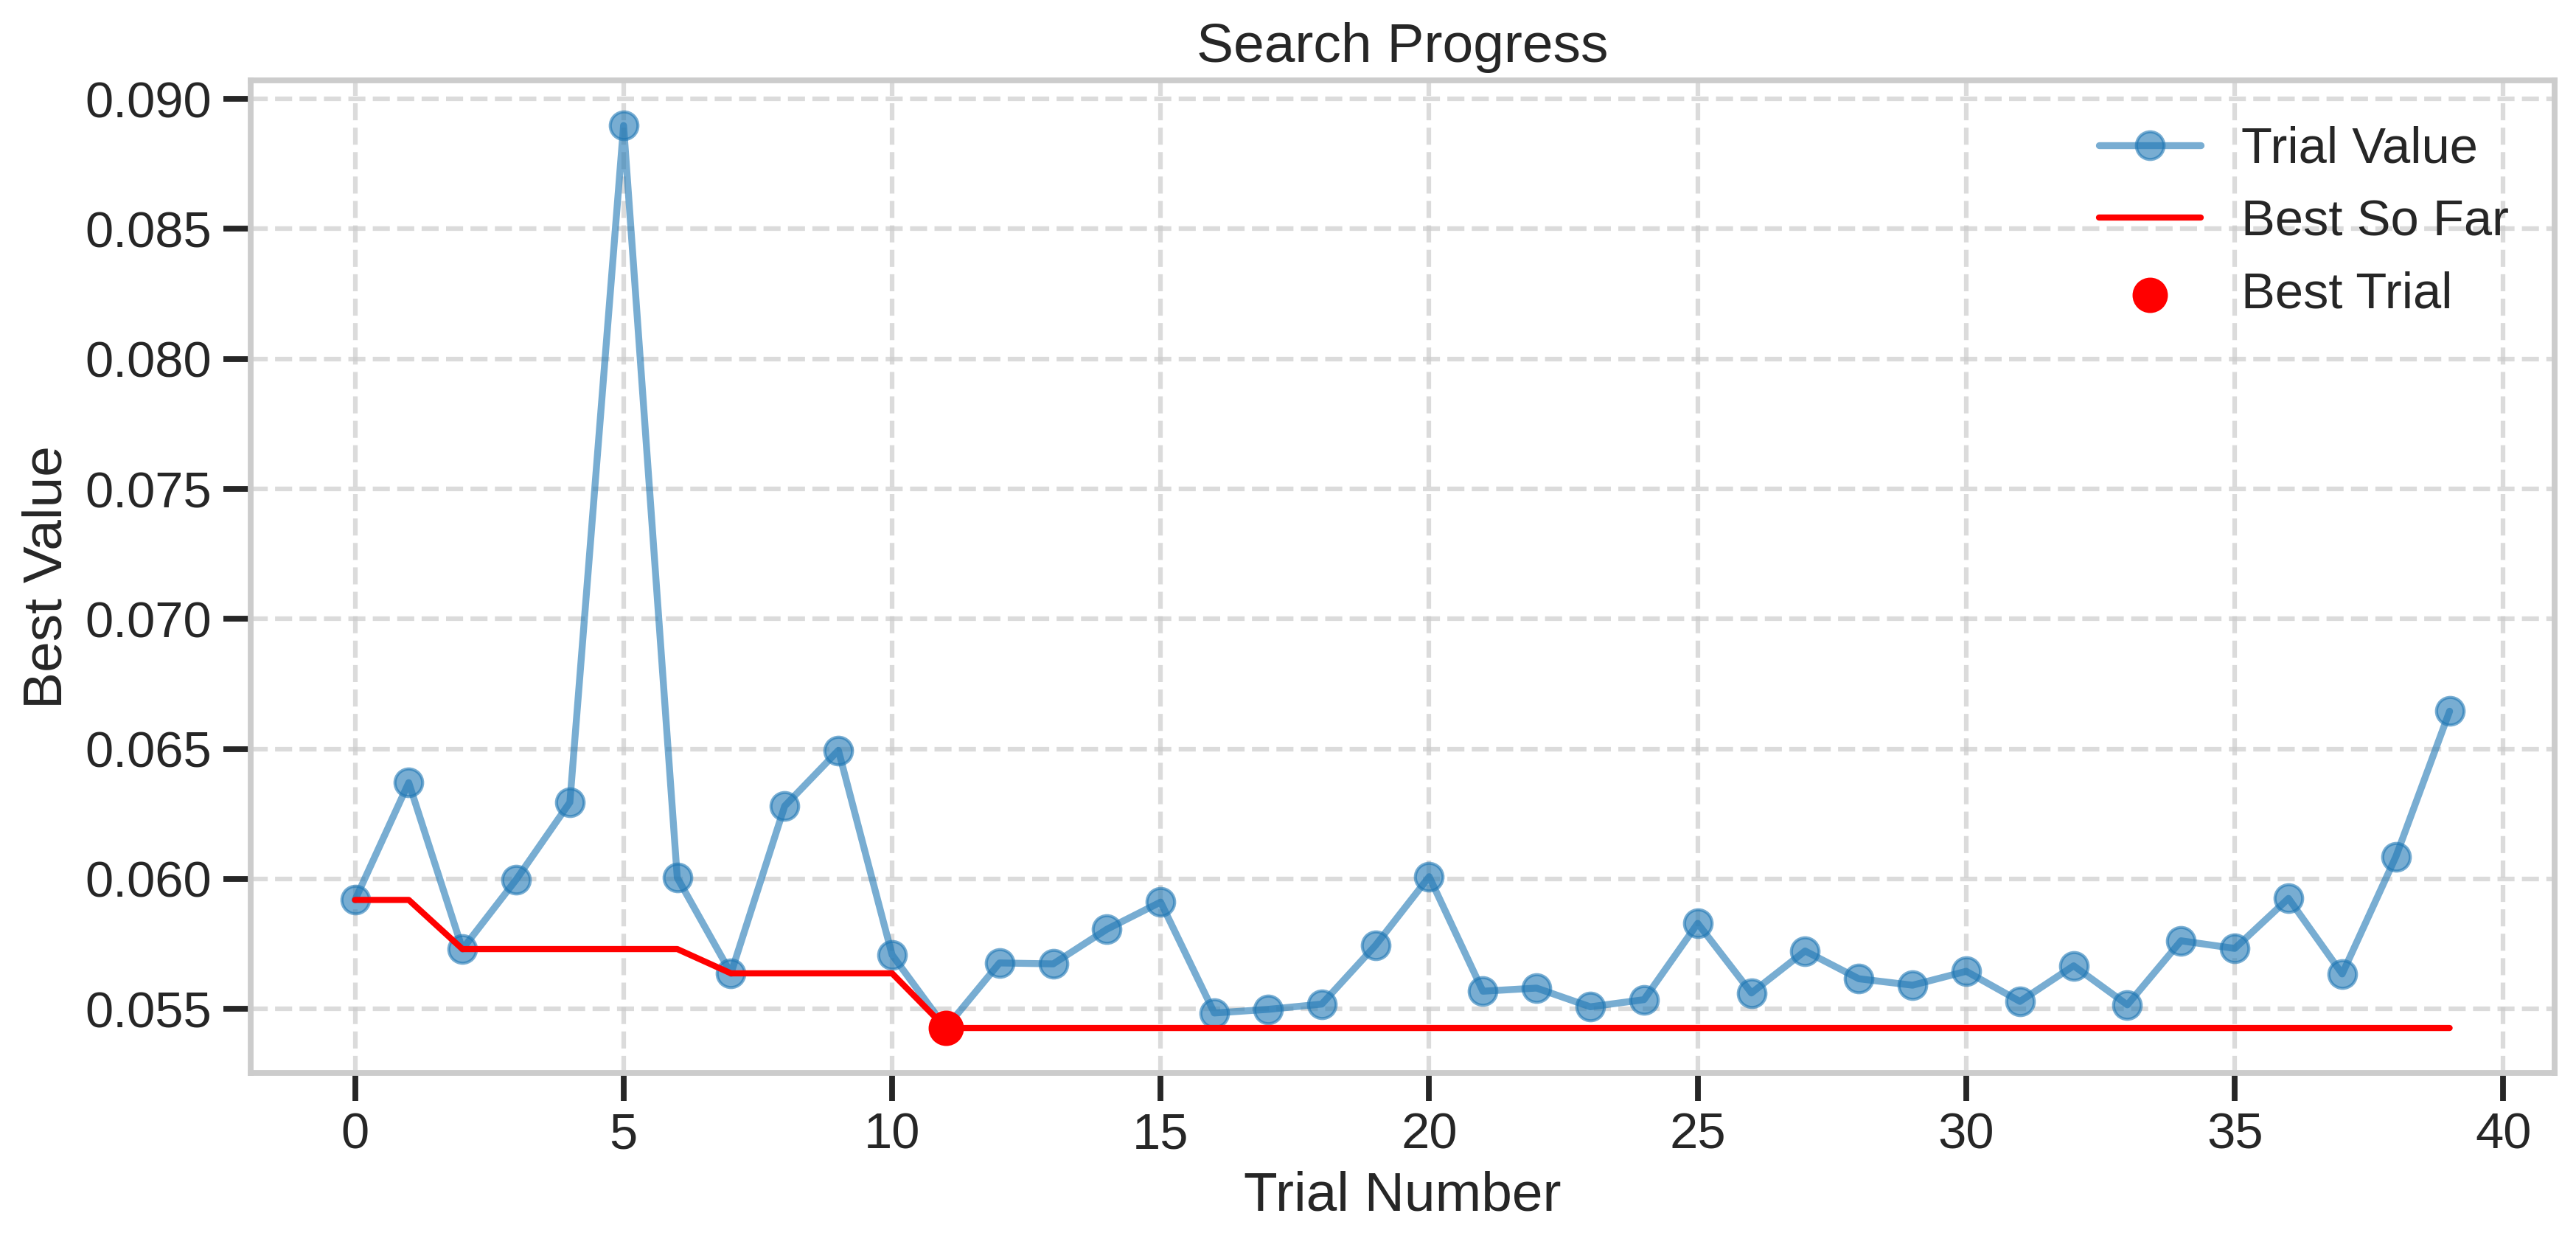
\includegraphics[width=\textwidth]{bayesian_search_progress.png}
\caption{Search progress}
\label{fig:bayesian_search_progress}
\end{figure}

Na grafe je možné sledovať, ako rýchlo Bayesian Search identifikoval najlepšiu hodnotu RMSE, ktorá sa stabilizovala už po niekoľkých pokusoch. V porovnaní s progresom vyhľadávania algoritmu Random Search pozorujeme prakticky opačnú situáciu, hoci najefektívnejšia kombinácia bola nájdená v bezprostrednej blízkosti výsledkov Random Search. Na začiatku možno vidieť vysokú volatilitu neefektívnych kombinácií, ale vďaka tomu, že Bayesian Search adaptívne hľadá kombinácie na základe predchádzajúcich výsledkov, a ako vidno na grafe, pri ďalšom hľadaní kombinácií sa výsledky nevyznačujú volatilitou, možno s istotou tvrdiť, že Bayesian Search má vyššiu efektívnosť v porovnaní s predchádzajúcim algoritmom. V prípade Random Search by sa dalo povedať, že mu "prialo šťastie" pri nájdení efektívnej kombinácie.

\subsection{Vizualizácia výsledkov Grid Search}

Grid Search bol záverečnou optimalizačnou fázou, v ktorej sme sa zamerali na dôkladné preskúmanie najperspektívnejších kombinácií hyperparametrov identifikovaných v predošlých experimentoch. Vďaka predchádzajúcej selekcii sme mohli obmedziť počet kombinácií a tým výrazne zvýšiť výpočtovú efektivitu bez kompromisu na kvalite výsledkov.

\subsubsection{Progres vyhľadávania (Search Progress)}
Graf vyhľadávania ukazuje priebeh znižovania hodnoty validačnej chyby RMSE. Aj napriek veľkému počtu testovaných konfigurácií bola najlepšia konfigurácia nájdená v relatívne skorých iteráciách.

\begin{figure}[ht!]
\centering
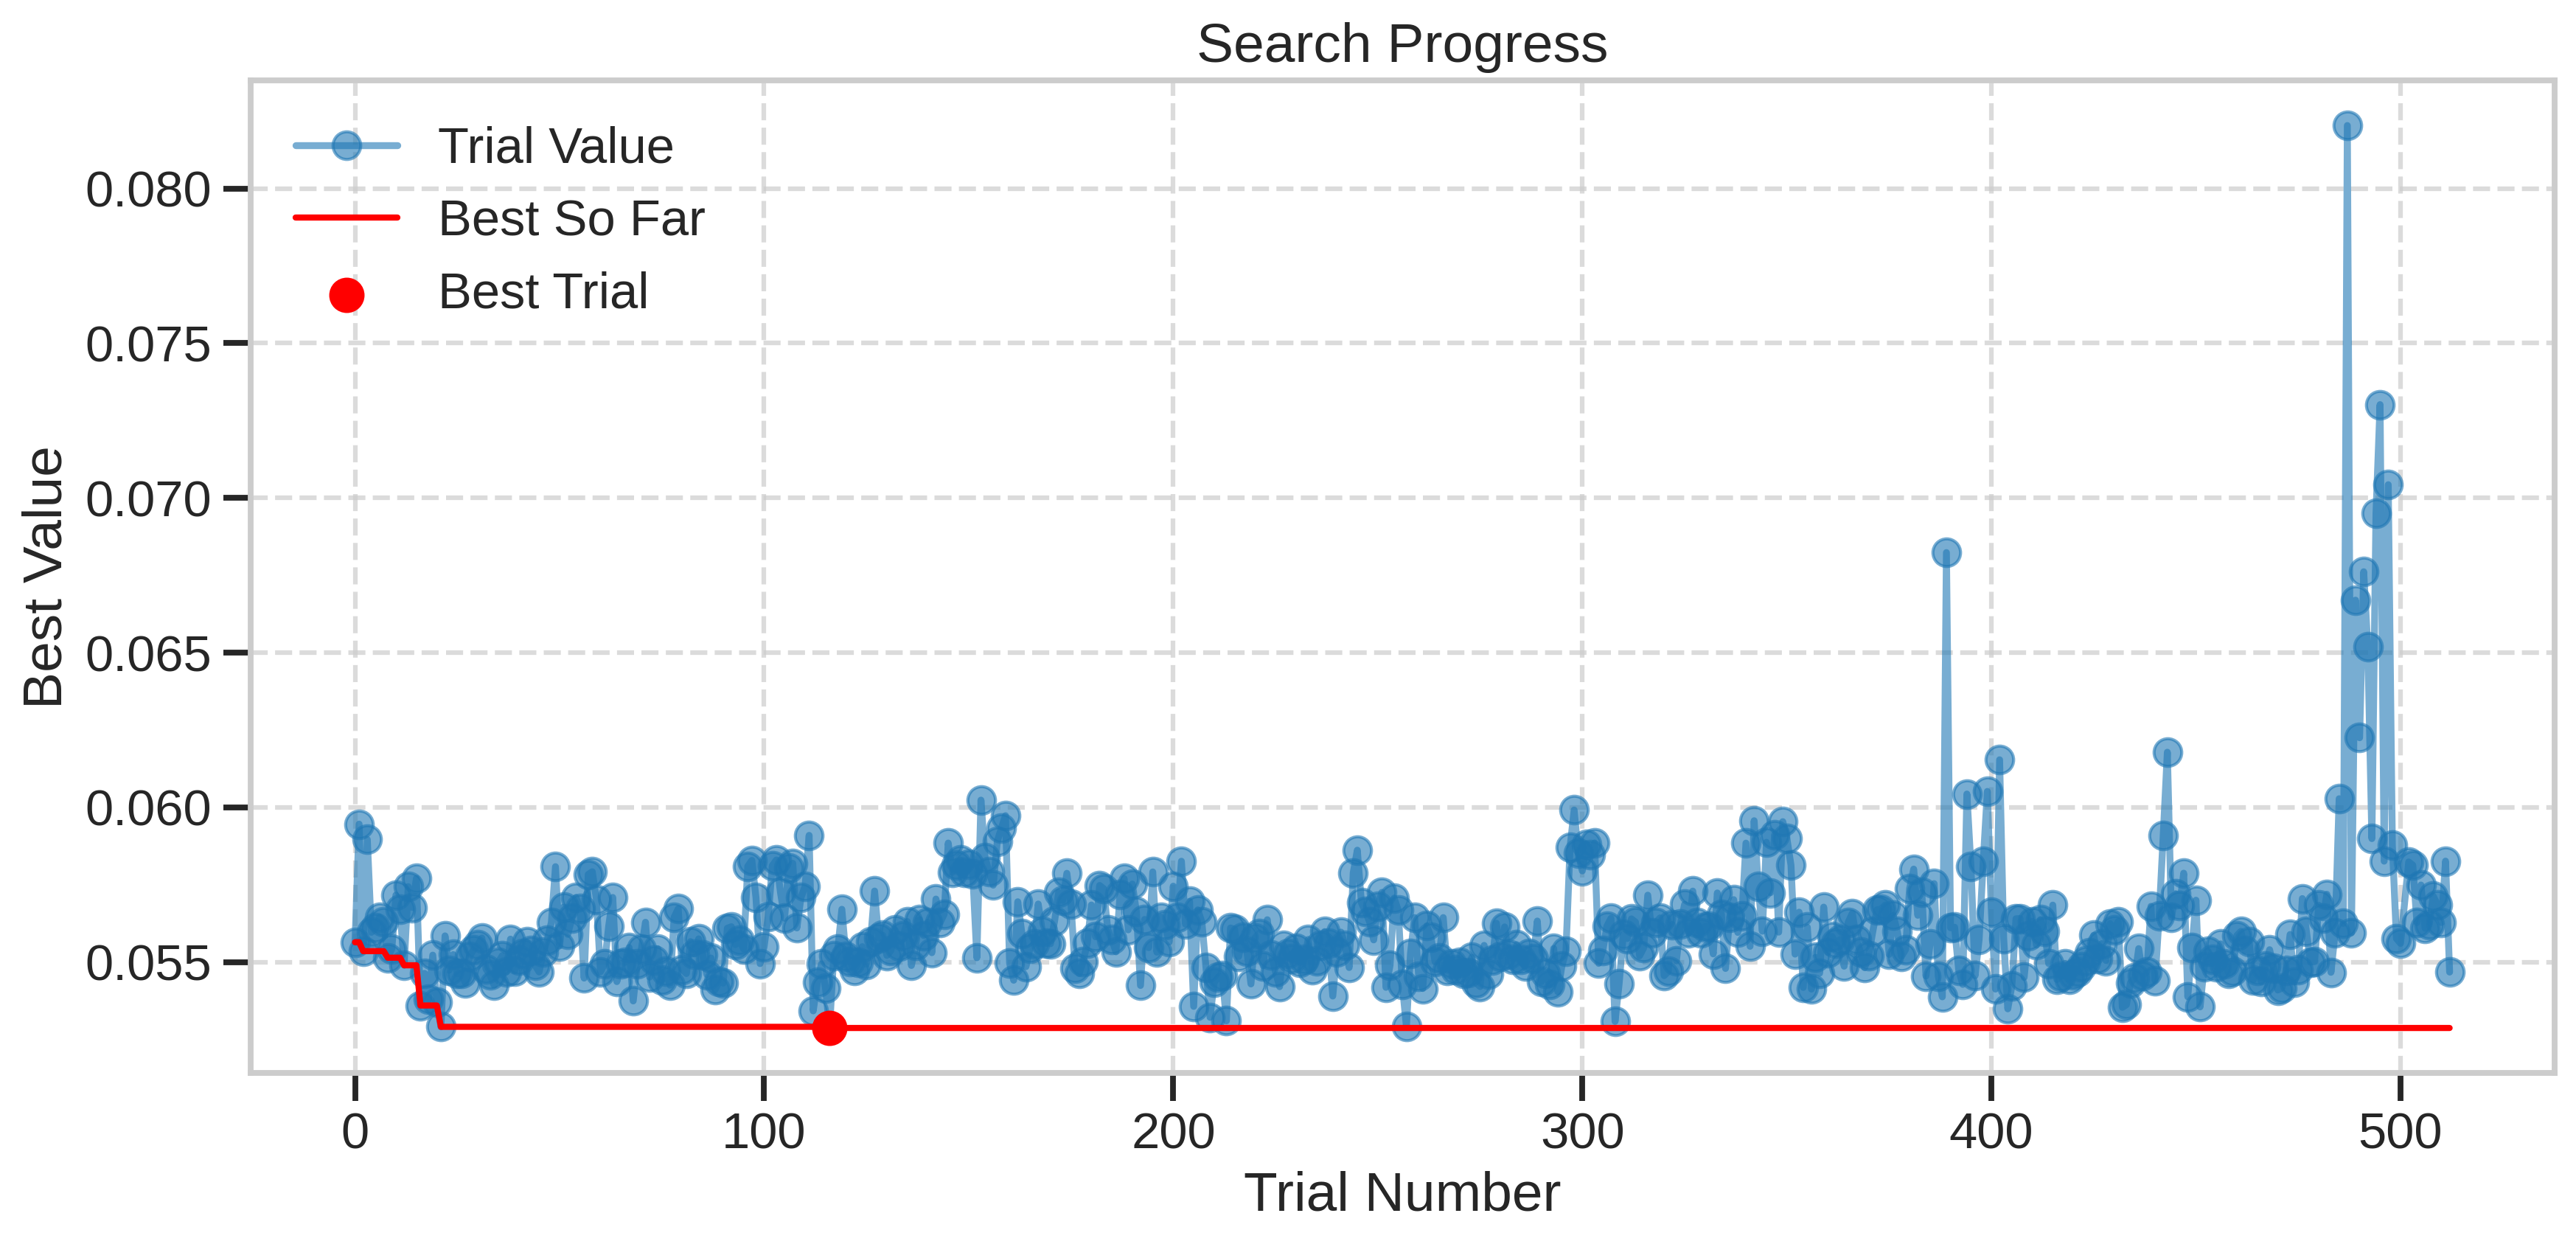
\includegraphics[width=\textwidth]{grid_search_search_progress.png}
\caption{Search progress}
\label{fig:grid_search_search_progress}
\end{figure}

\newpage

\subsubsection{Krivky učenia (Learning Curves)}
Porovnanie vývoja loss a MAE pre top 3 pokusy počas tréningu a validácie odhaľuje stabilné učenie modelu s dobrou schopnosťou generalizácie. Z grafov vyplýva, že overfitting bol minimálny vďaka použitým technikám ako dropout a early stopping.

\begin{figure}[ht!]
\centering
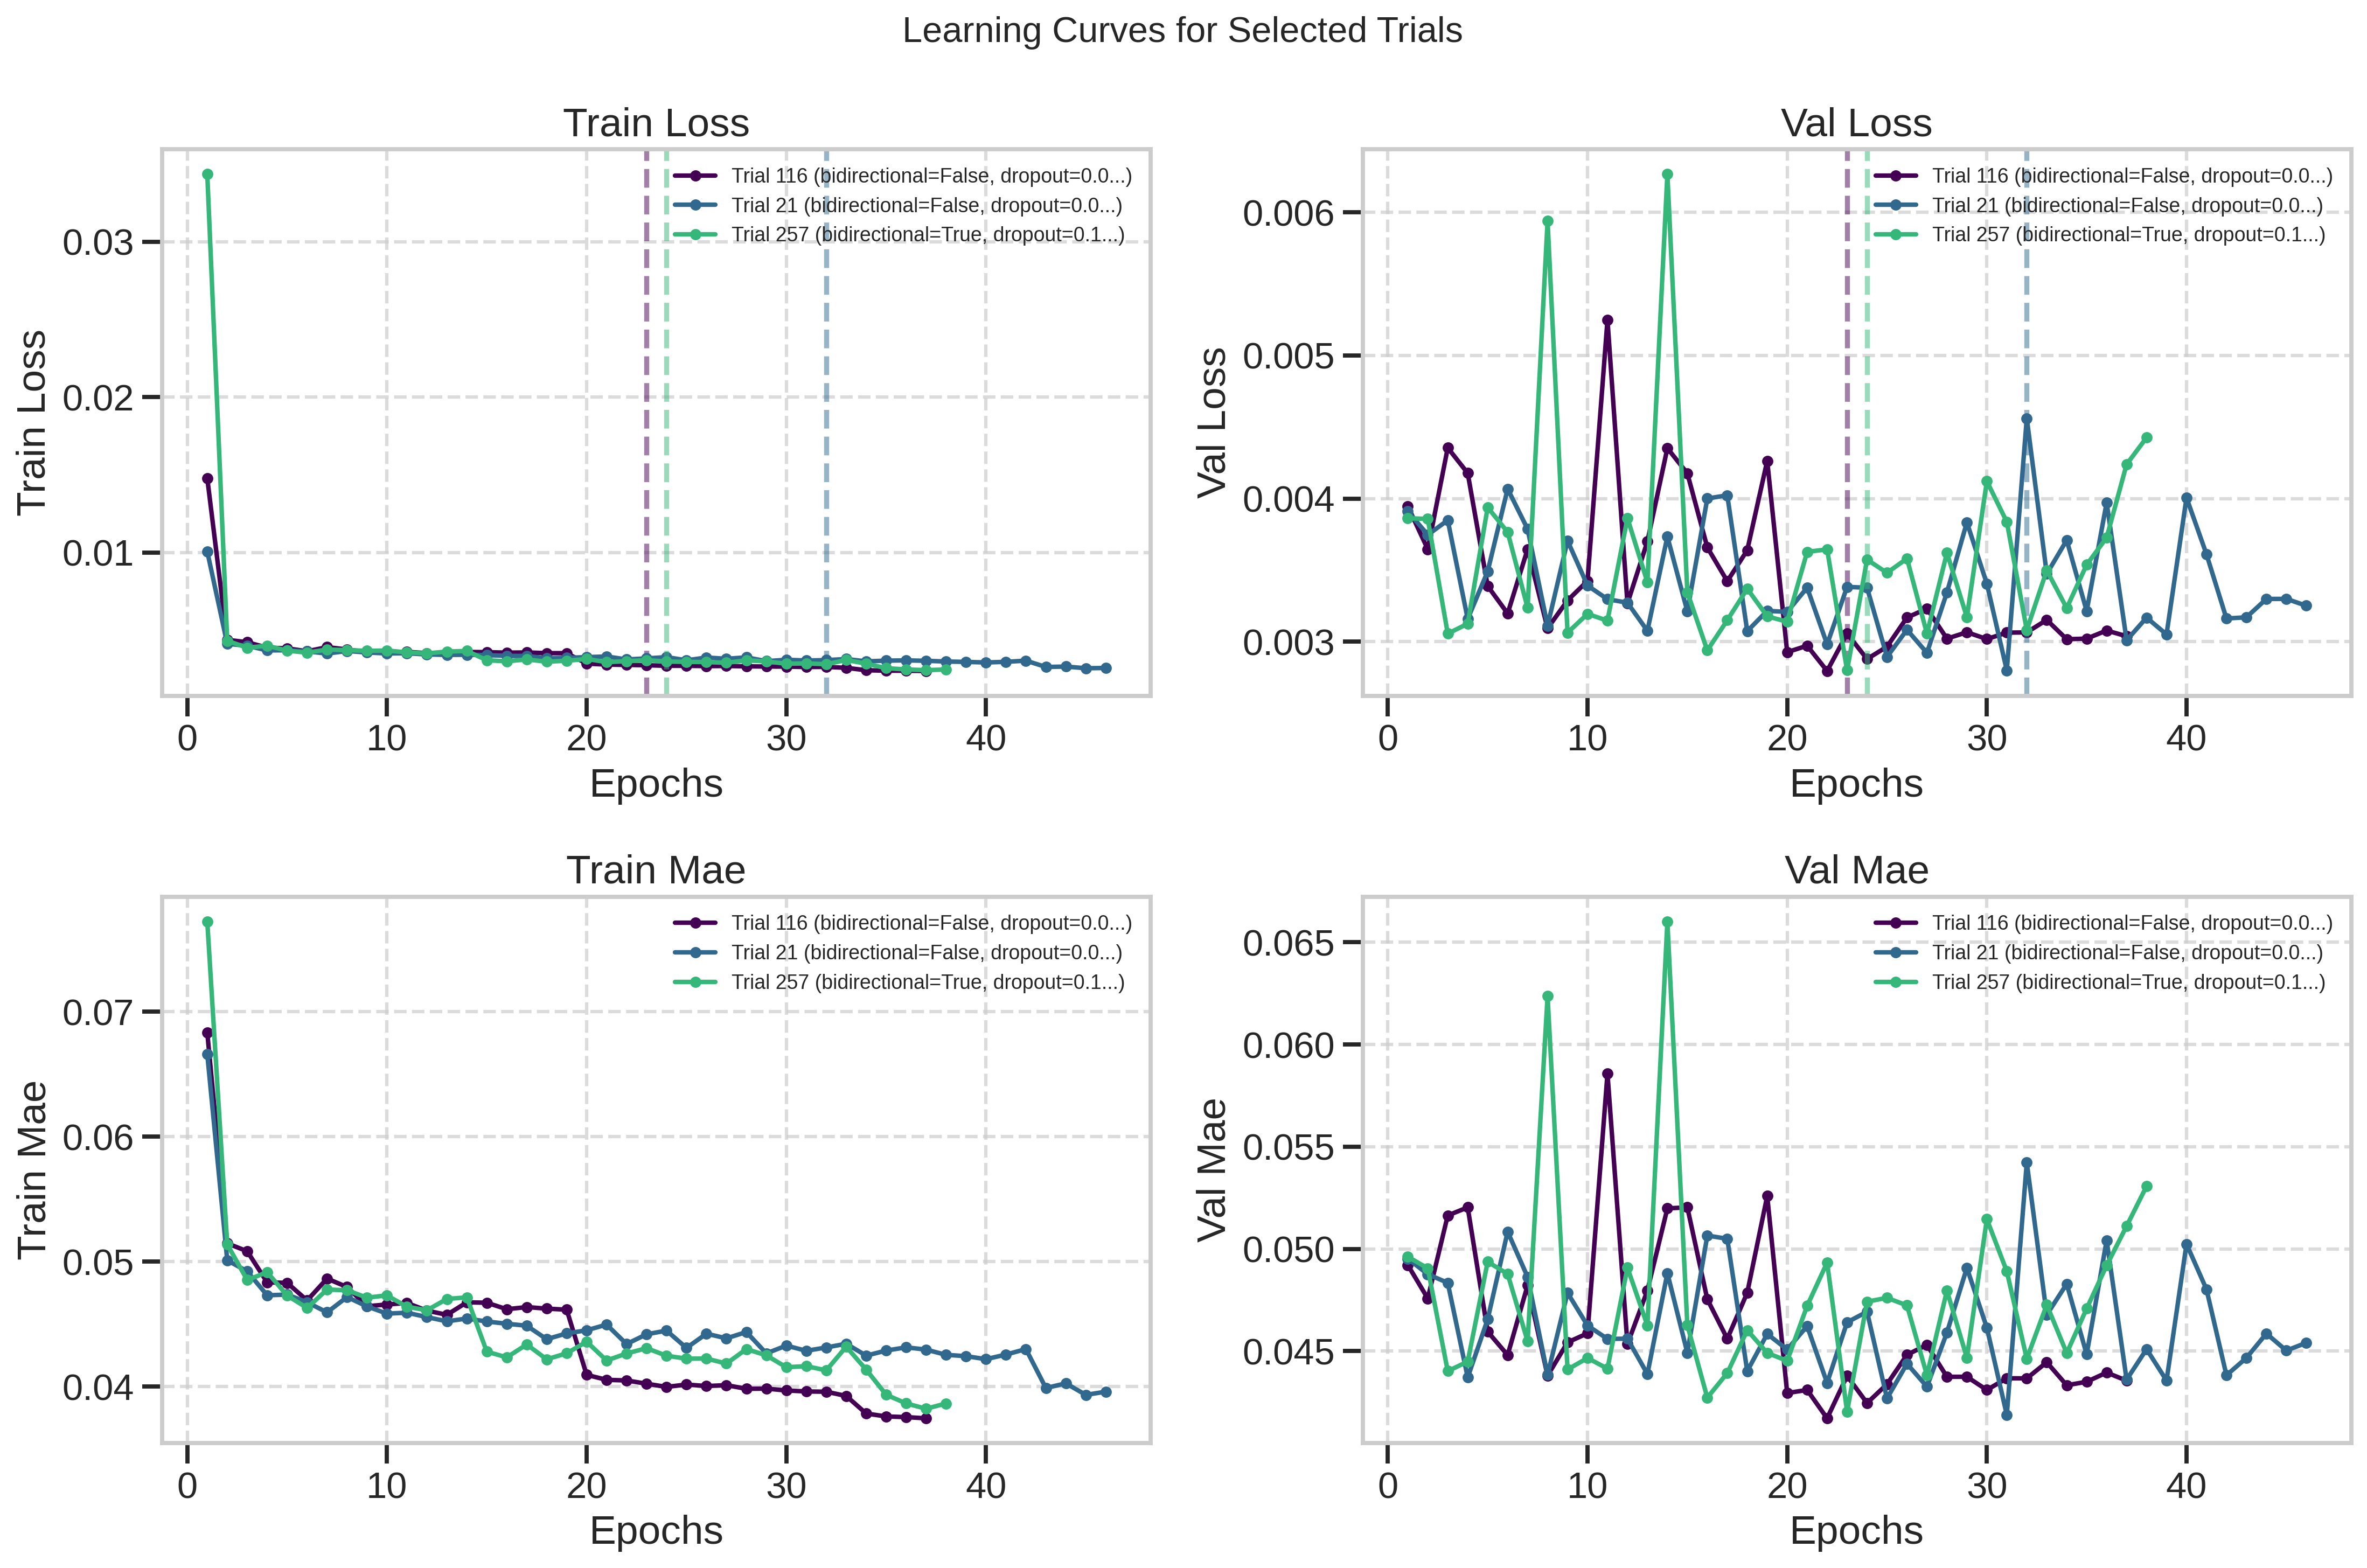
\includegraphics[width=\textwidth]{grid_search_learning_curves.png}
\caption{Learning curves}
\label{fig:grid_search_learning_curves}
\end{figure}

Výsledky sú veľmi podobné výsledkom predchádzajúcich vyhľadávaní. V tomto jedinečnom prípade najlepšie 3 kombinácie preukázali dobrú schopnosť generalizácie a prakticky lineárnu tendenciu znižovania funkcie straty pri validácii zodpovedajúcu trénovaniu, a to napriek štandardnej volatilite na začiatku.

\newpage

\subsubsection{Vzťah medzi epochami a stratou (Epochs vs Loss)}
Tento graf poskytuje informácie o dynamike učenia počas jednotlivých epoch. Modely dosahovali veľmi nízke chyby už v prvých 20 epochách, pričom ďalšie zlepšovanie bolo pozvoľné.

\begin{figure}[ht!]
\centering
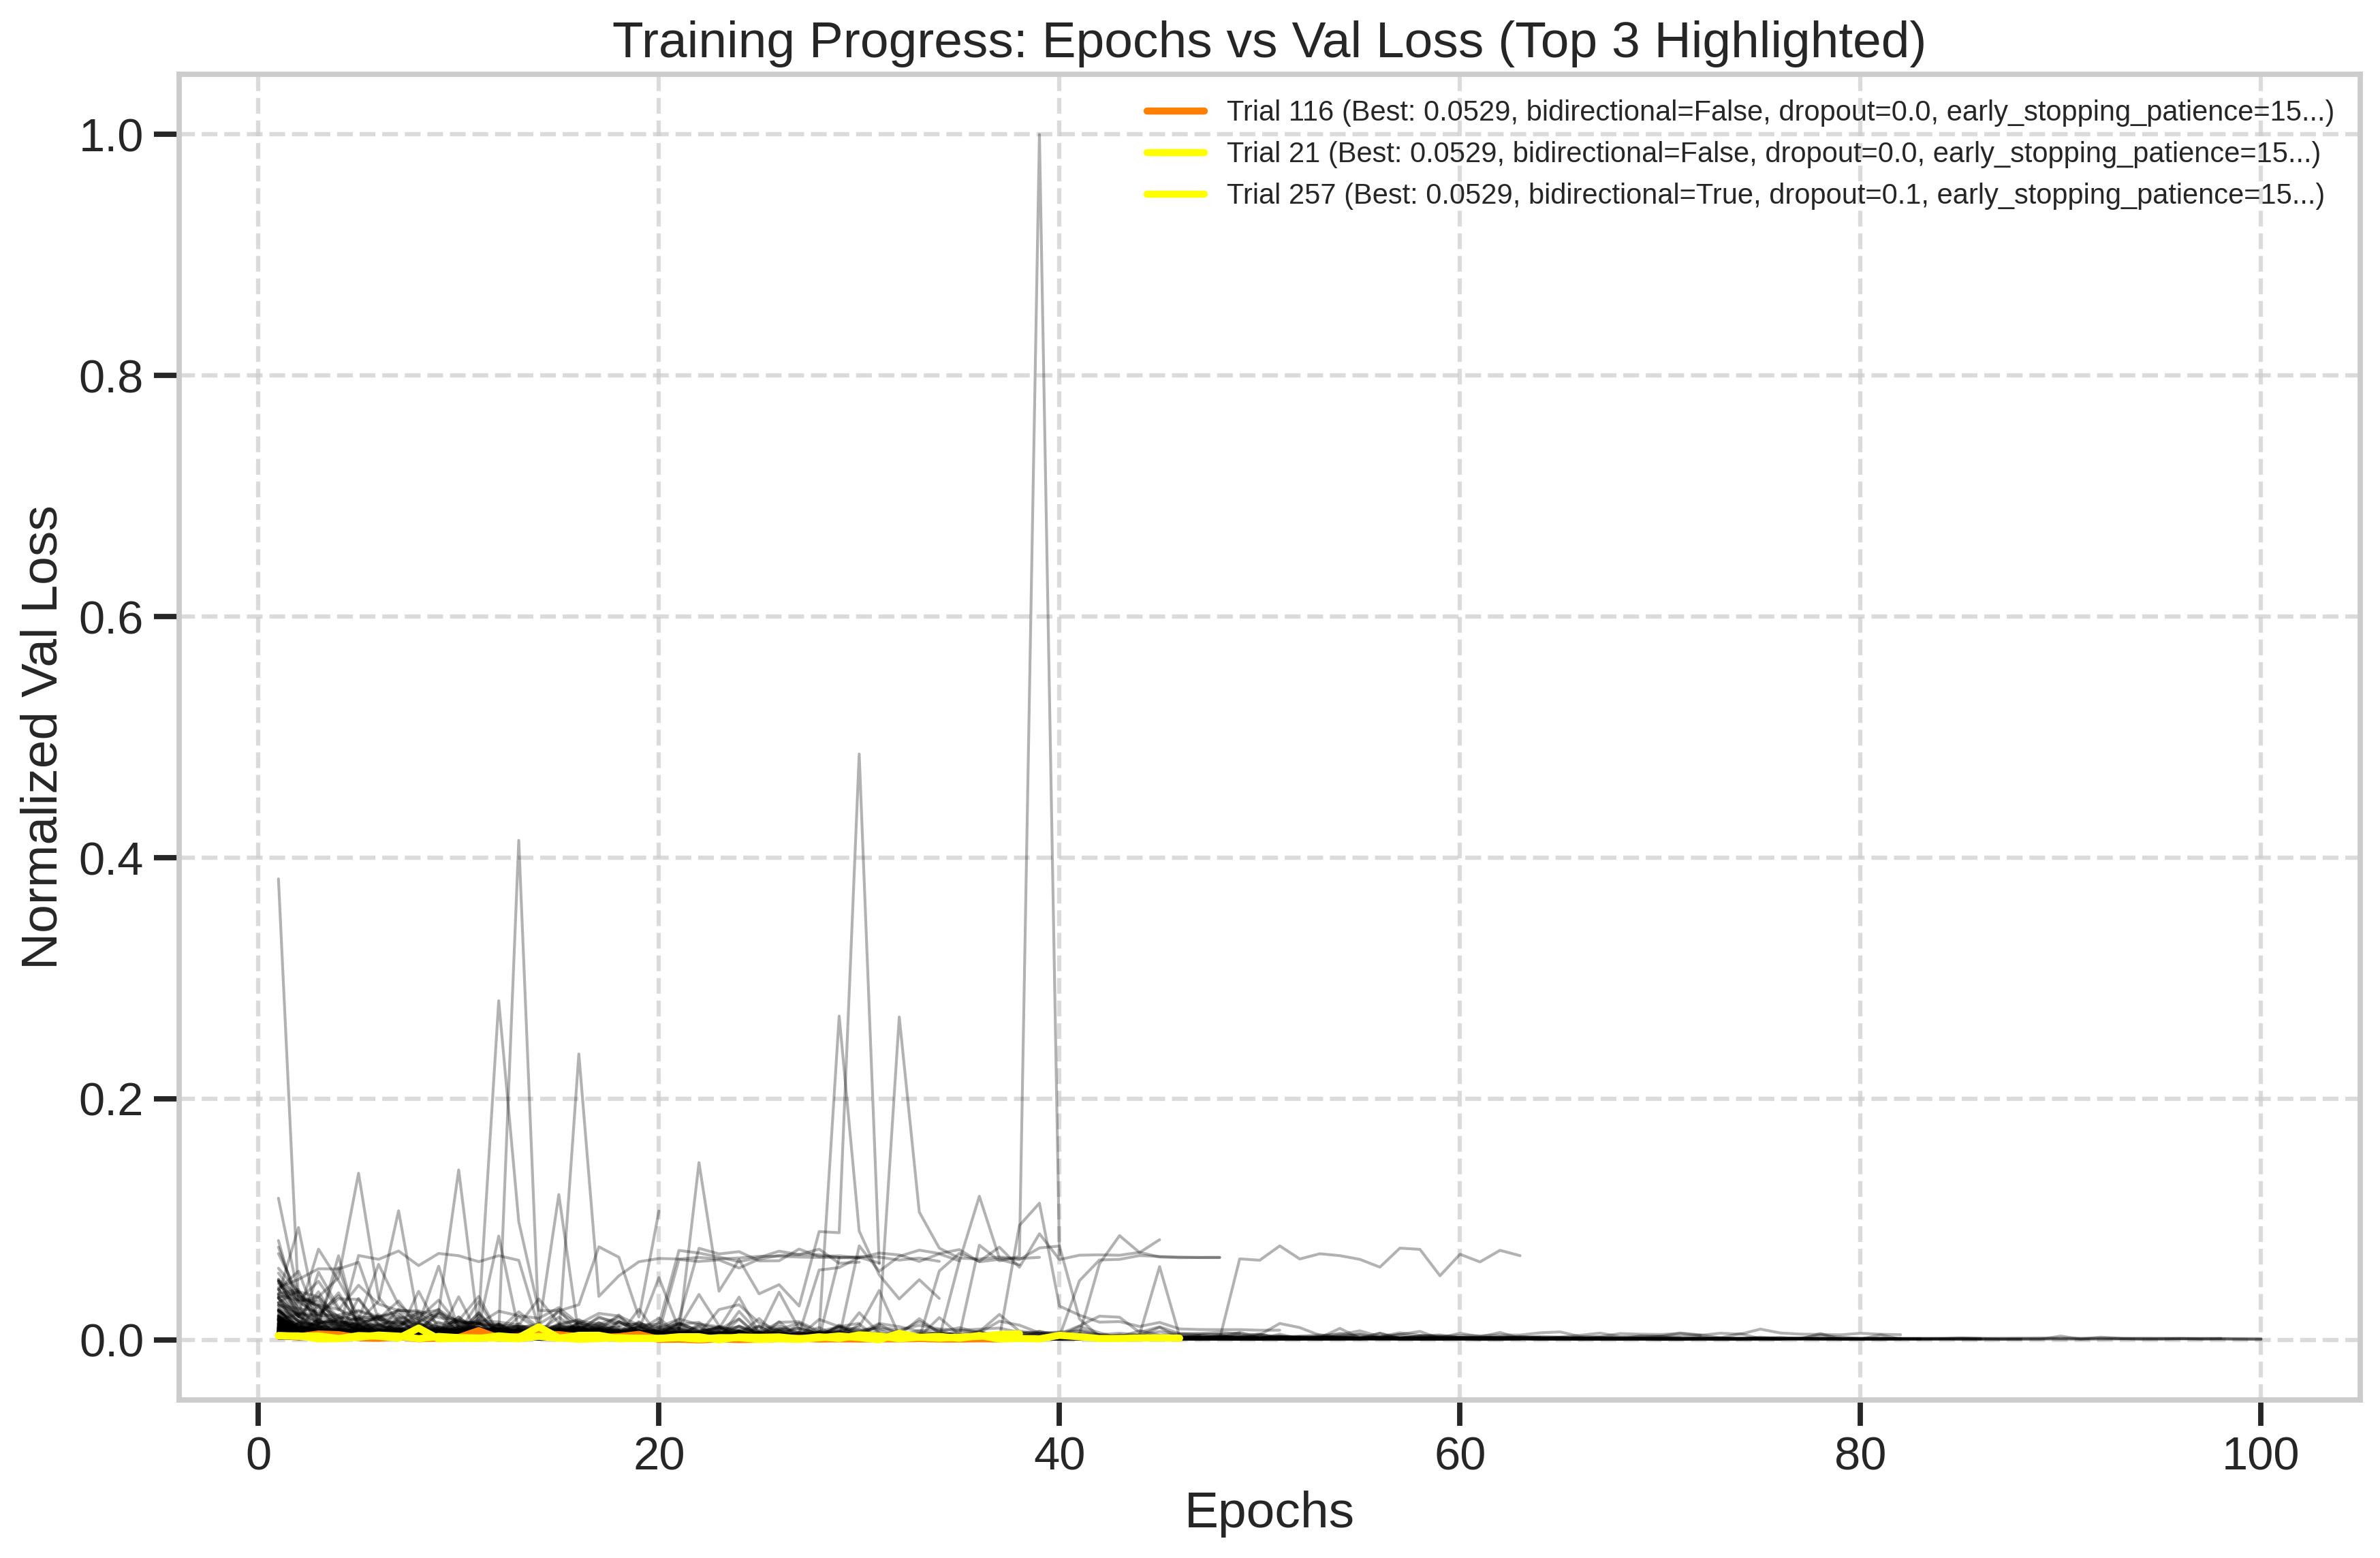
\includegraphics[width=\textwidth]{grid_search_epochs_vs_loss.png}
\caption{Epochs vs Loss}
\label{fig:grid_search_epochs_vs_loss}
\end{figure}

Zúženie siete hyperparametrov poslúžilo nielen ako dobrá praktika pre zrýchlenie vyhľadávania, ale sa tiež odrazilo na výsledkoch. Absolútna väčšina kombinácií preukázala vynikajúcu konvergenciu, lineárne klesala a v najlepších prípadoch vykazovala vysokú efektivitu počas prvej polovice epoch. Samozrejme, existujú aj ojedinelé prípady vykazujúce enormnú volatilitu a neefektívnosť. Najlepšie 3 kombinácie sa navzájom líšia hodnotami funkcie straty menej než o 4 desatinné miesta, čo demonštruje vynikajúci prieskum oblasti efektívnych hyperparametrov.

\newpage

\subsubsection{Vplyv skrytej vrstvy (Hidden Size Influence)}
Z grafu je zrejmé, že vyššie hodnoty skrytých vrstiev (napr. 512) neznamenali automaticky lepšiu výkonnosť. Optimálne výsledky boli dosiahnuté aj pri nižších hodnotách ako 64 alebo 128, čo poukazuje na potrebu citlivej optimalizácie tohto parametra.

\begin{figure}[ht!]
\centering
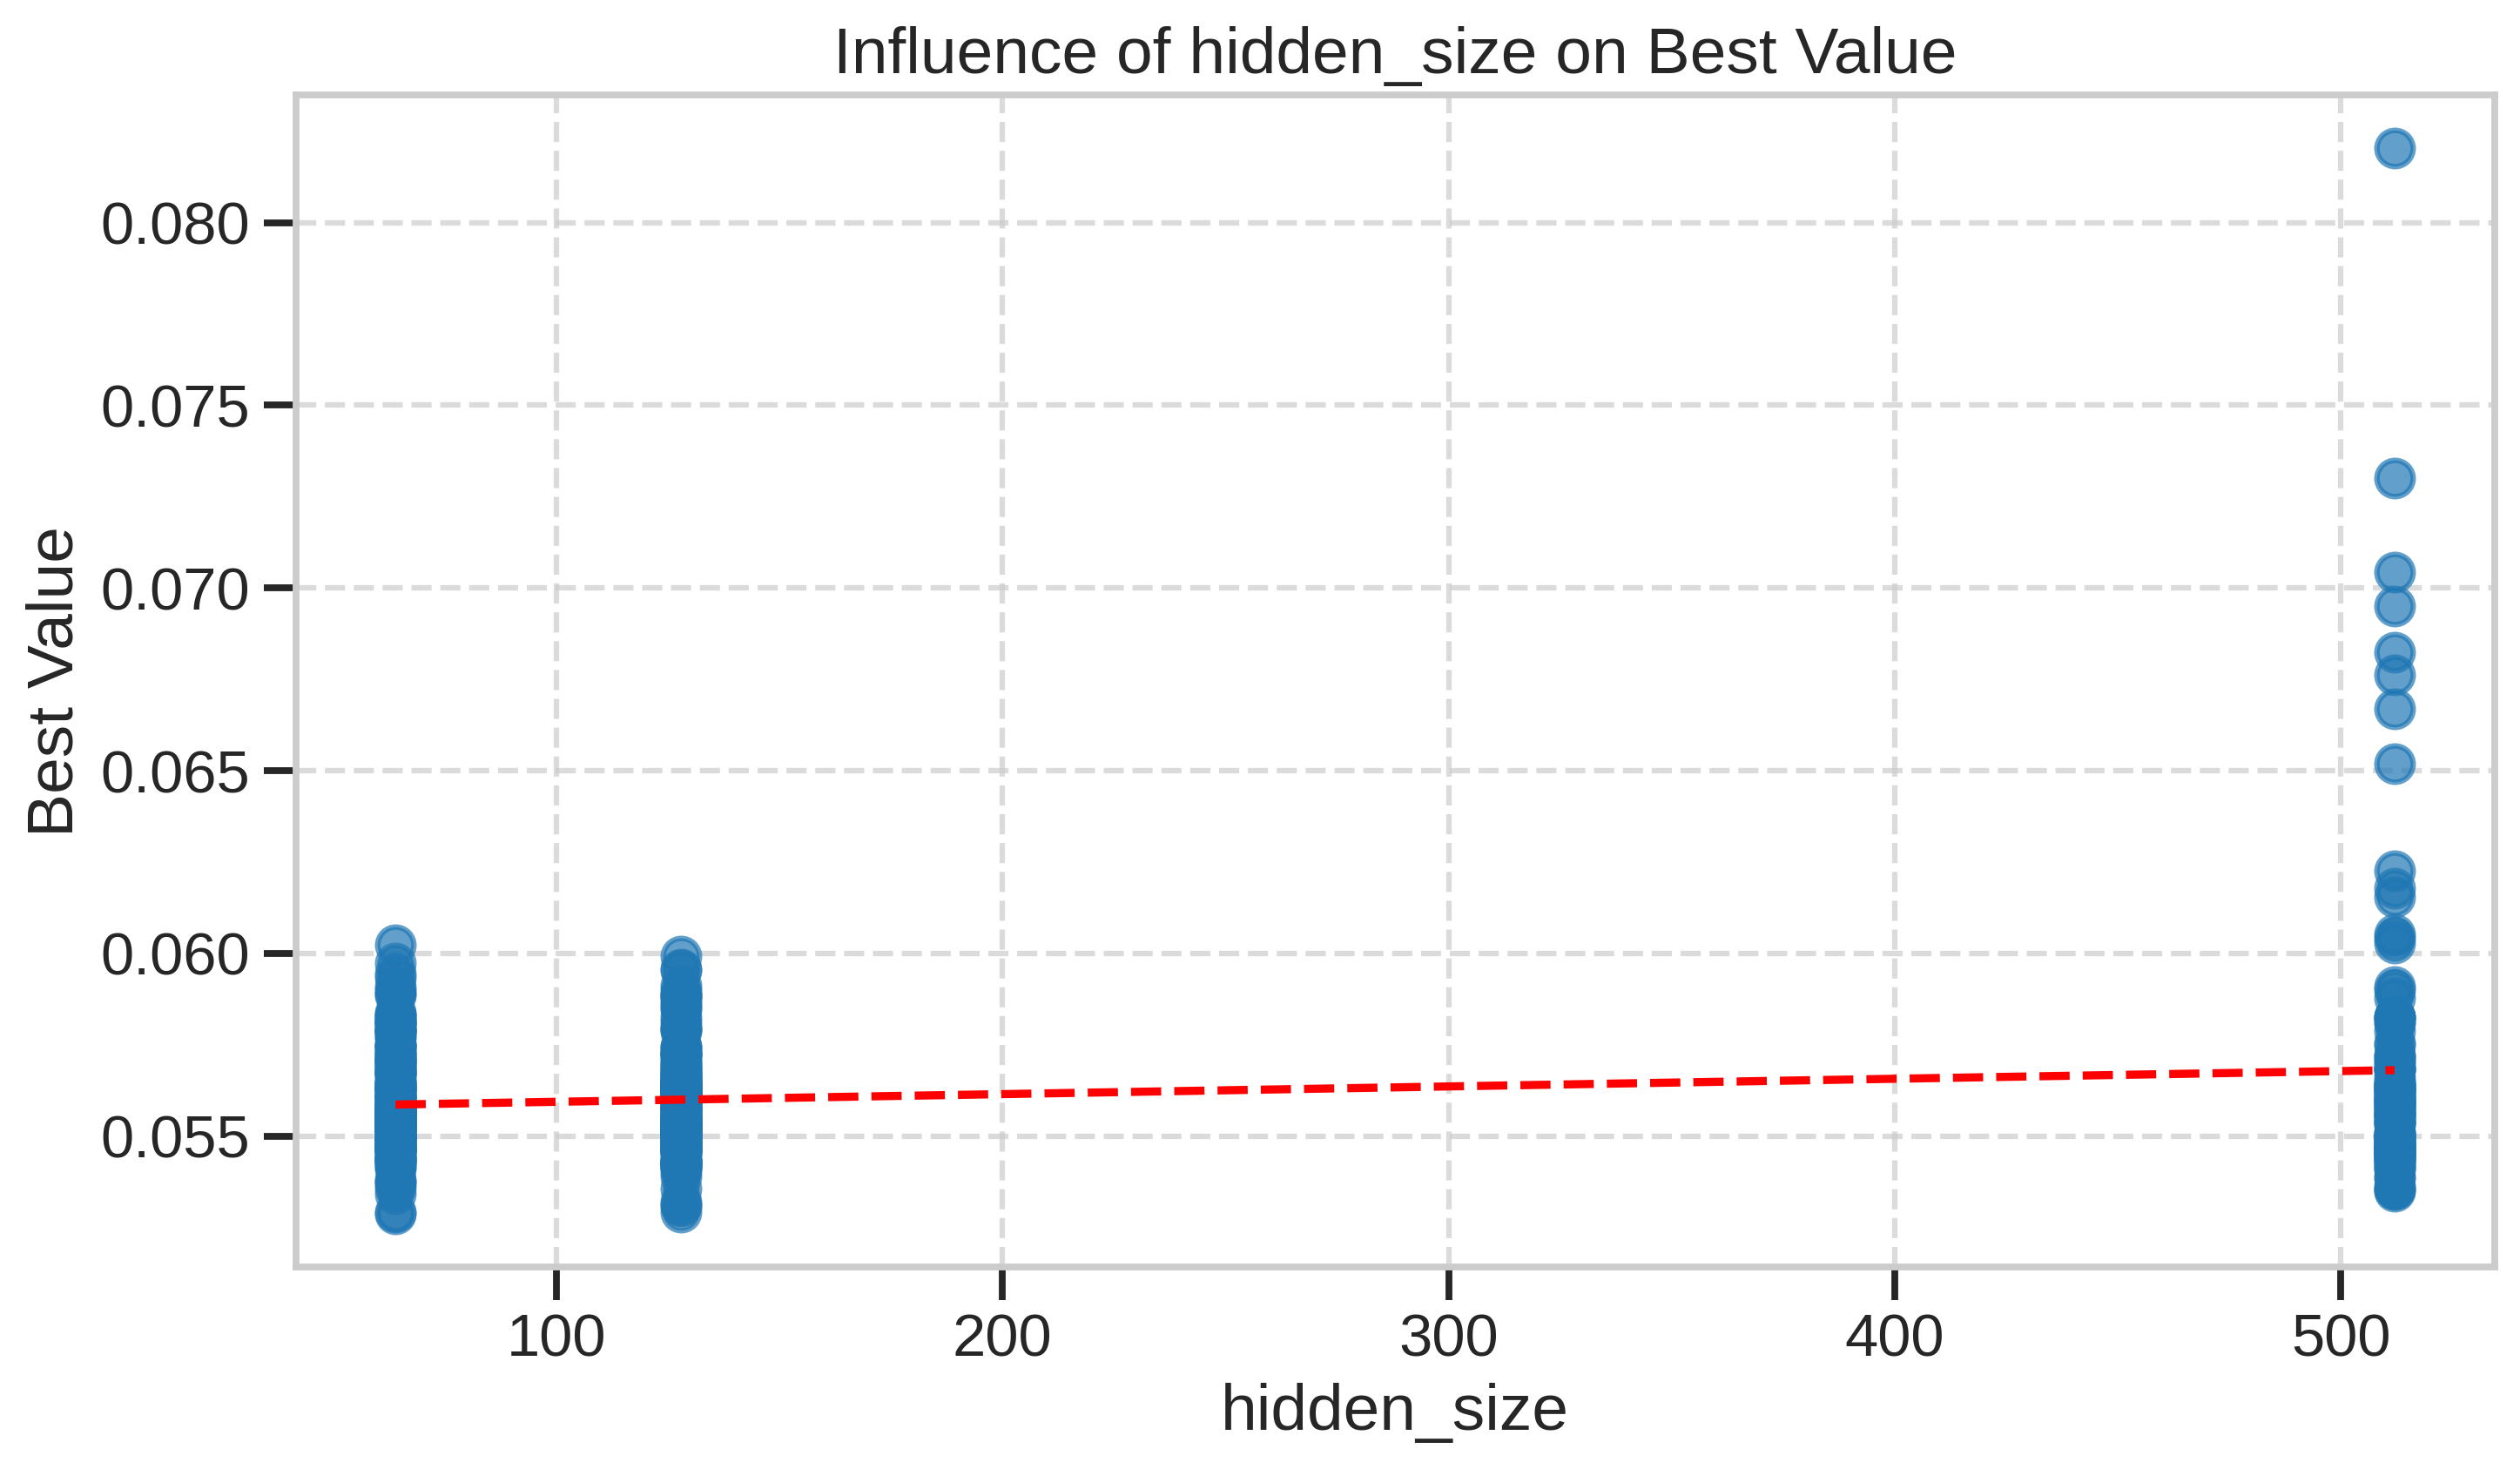
\includegraphics[width=\textwidth]{grid_search_hidden_size_influence.png}
\caption{Hidden size influence}
\label{fig:grid_search_hidden_size_influence}
\end{figure}

Výsledok je veľmi podobný predchádzajúcim algoritmom vyhľadávania, pričom sa zachovala tendencia od väčšej veľkosti blokov k menšej. Zároveň názorne vidíme, že hodnoty pre väčšie veľkosti blokov vykazujú veľký rozptyl a volatilitu v porovnaní s menšími veľkosťami.

\newpage

\subsubsection{Korelácia parametrov s výkonom (Parameter Correlation)}
Korelácia medzi jednotlivými hyperparametrami a výkonom modelu ukazuje, že najväčší negatívny vplyv mal počet vrstiev, zatiaľ čo hidden size a learning rate boli mierne pozitívne korelované s lepšou výkonnosťou. Tieto zistenia podporujú výber jednoduchšej, ale dobre nastavenej architektúry.

\begin{figure}[ht!]
\centering
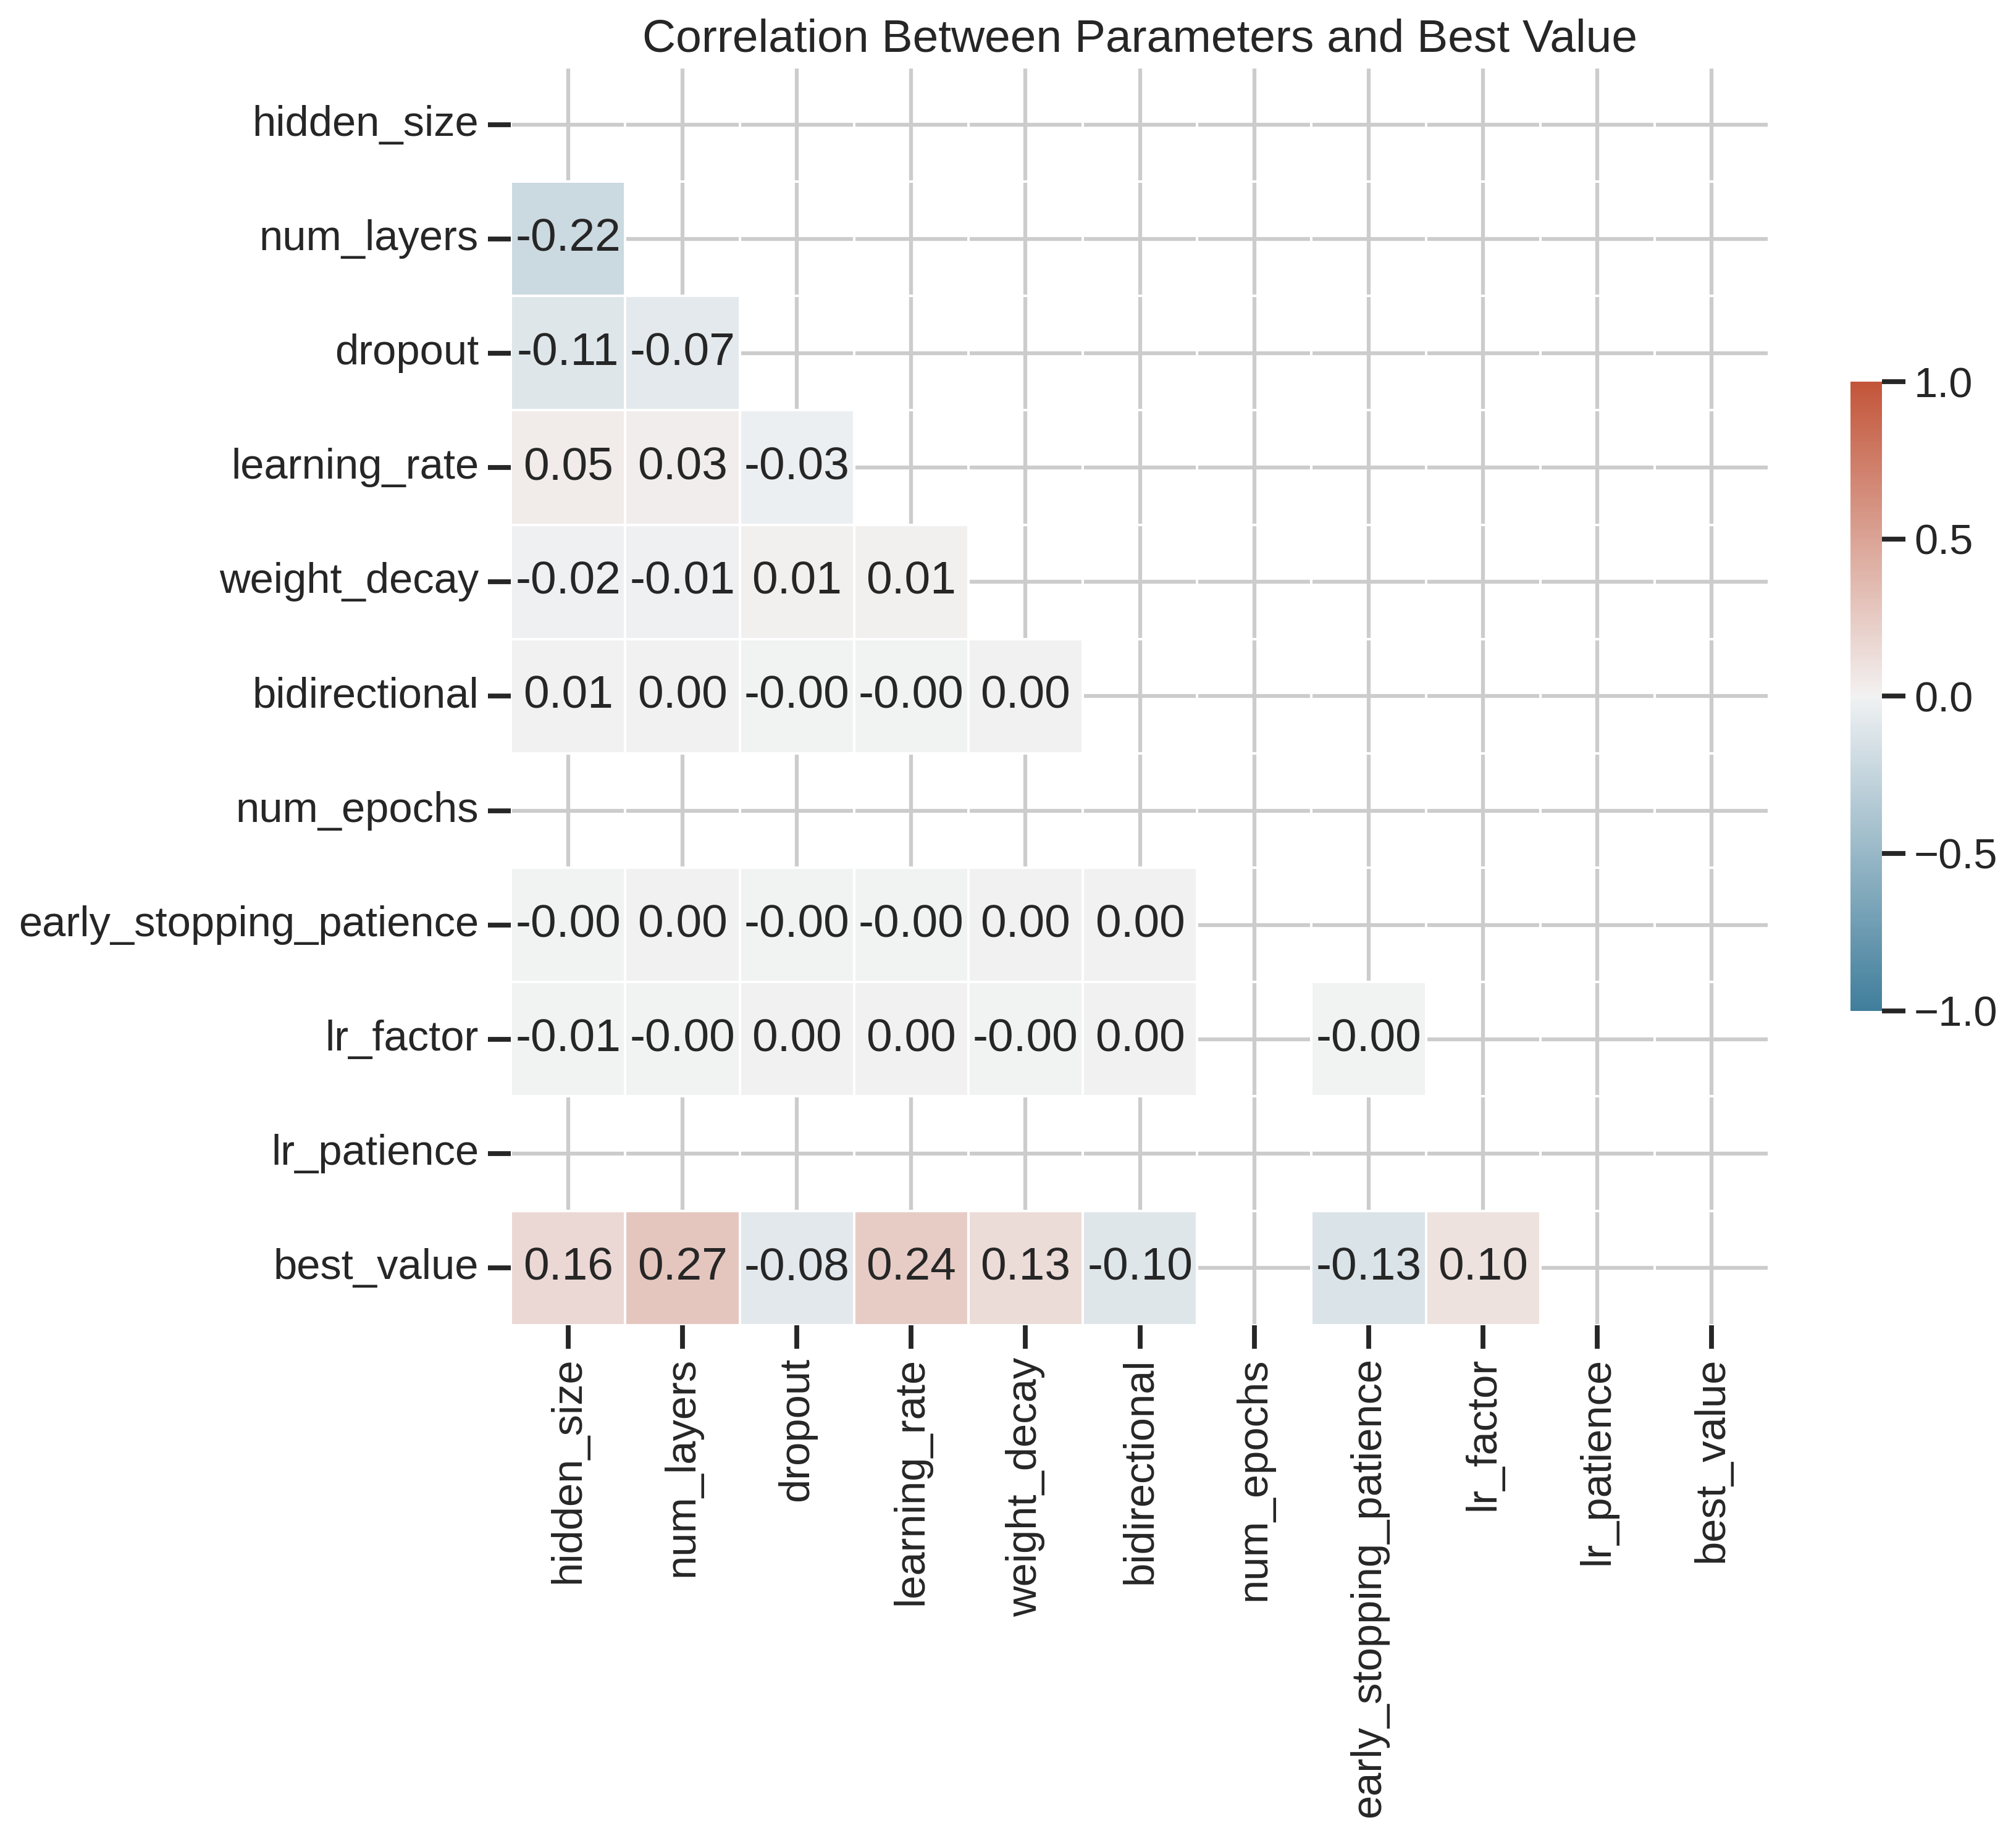
\includegraphics[width=\textwidth]{grid_search_parameter_correlation.png}
\caption{Parameter correlation}
\label{fig:grid_search_parameter_correlation}
\end{figure}

\subsection{Vizualizácia výsledkov modelu natrénovaného na najlepších parametroch}

Po ukončení optimalizácie pomocou Grid Search a identifikácii najlepšej kombinácie hyperparametrov bola natrénovaná finálna GRU modelová architektúra. Tento model bol detailne analyzovaný z pohľadu vývoja učiacich kriviek, dynamiky učiacej rýchlosti, ako aj hodnotení širokého spektra metrických indikátorov.

\subsubsection{Evolúcia chýb a dynamika tréningu}

Vizualizácia \textbf{Error Metrics Evolution} ilustruje, ako sa vyvíjali chyby typu MAPE \ref{mape}, SMAPE \ref{smape} a PEAK\_ERROR \ref{pe} v priebehu tréningu a validácie. Po počiatočnom prudkom poklese sa metriky ustálili a dosiahli stabilné hodnoty, čo naznačuje dobrú generalizáciu modelu.

\begin{figure}[ht!]
\centering
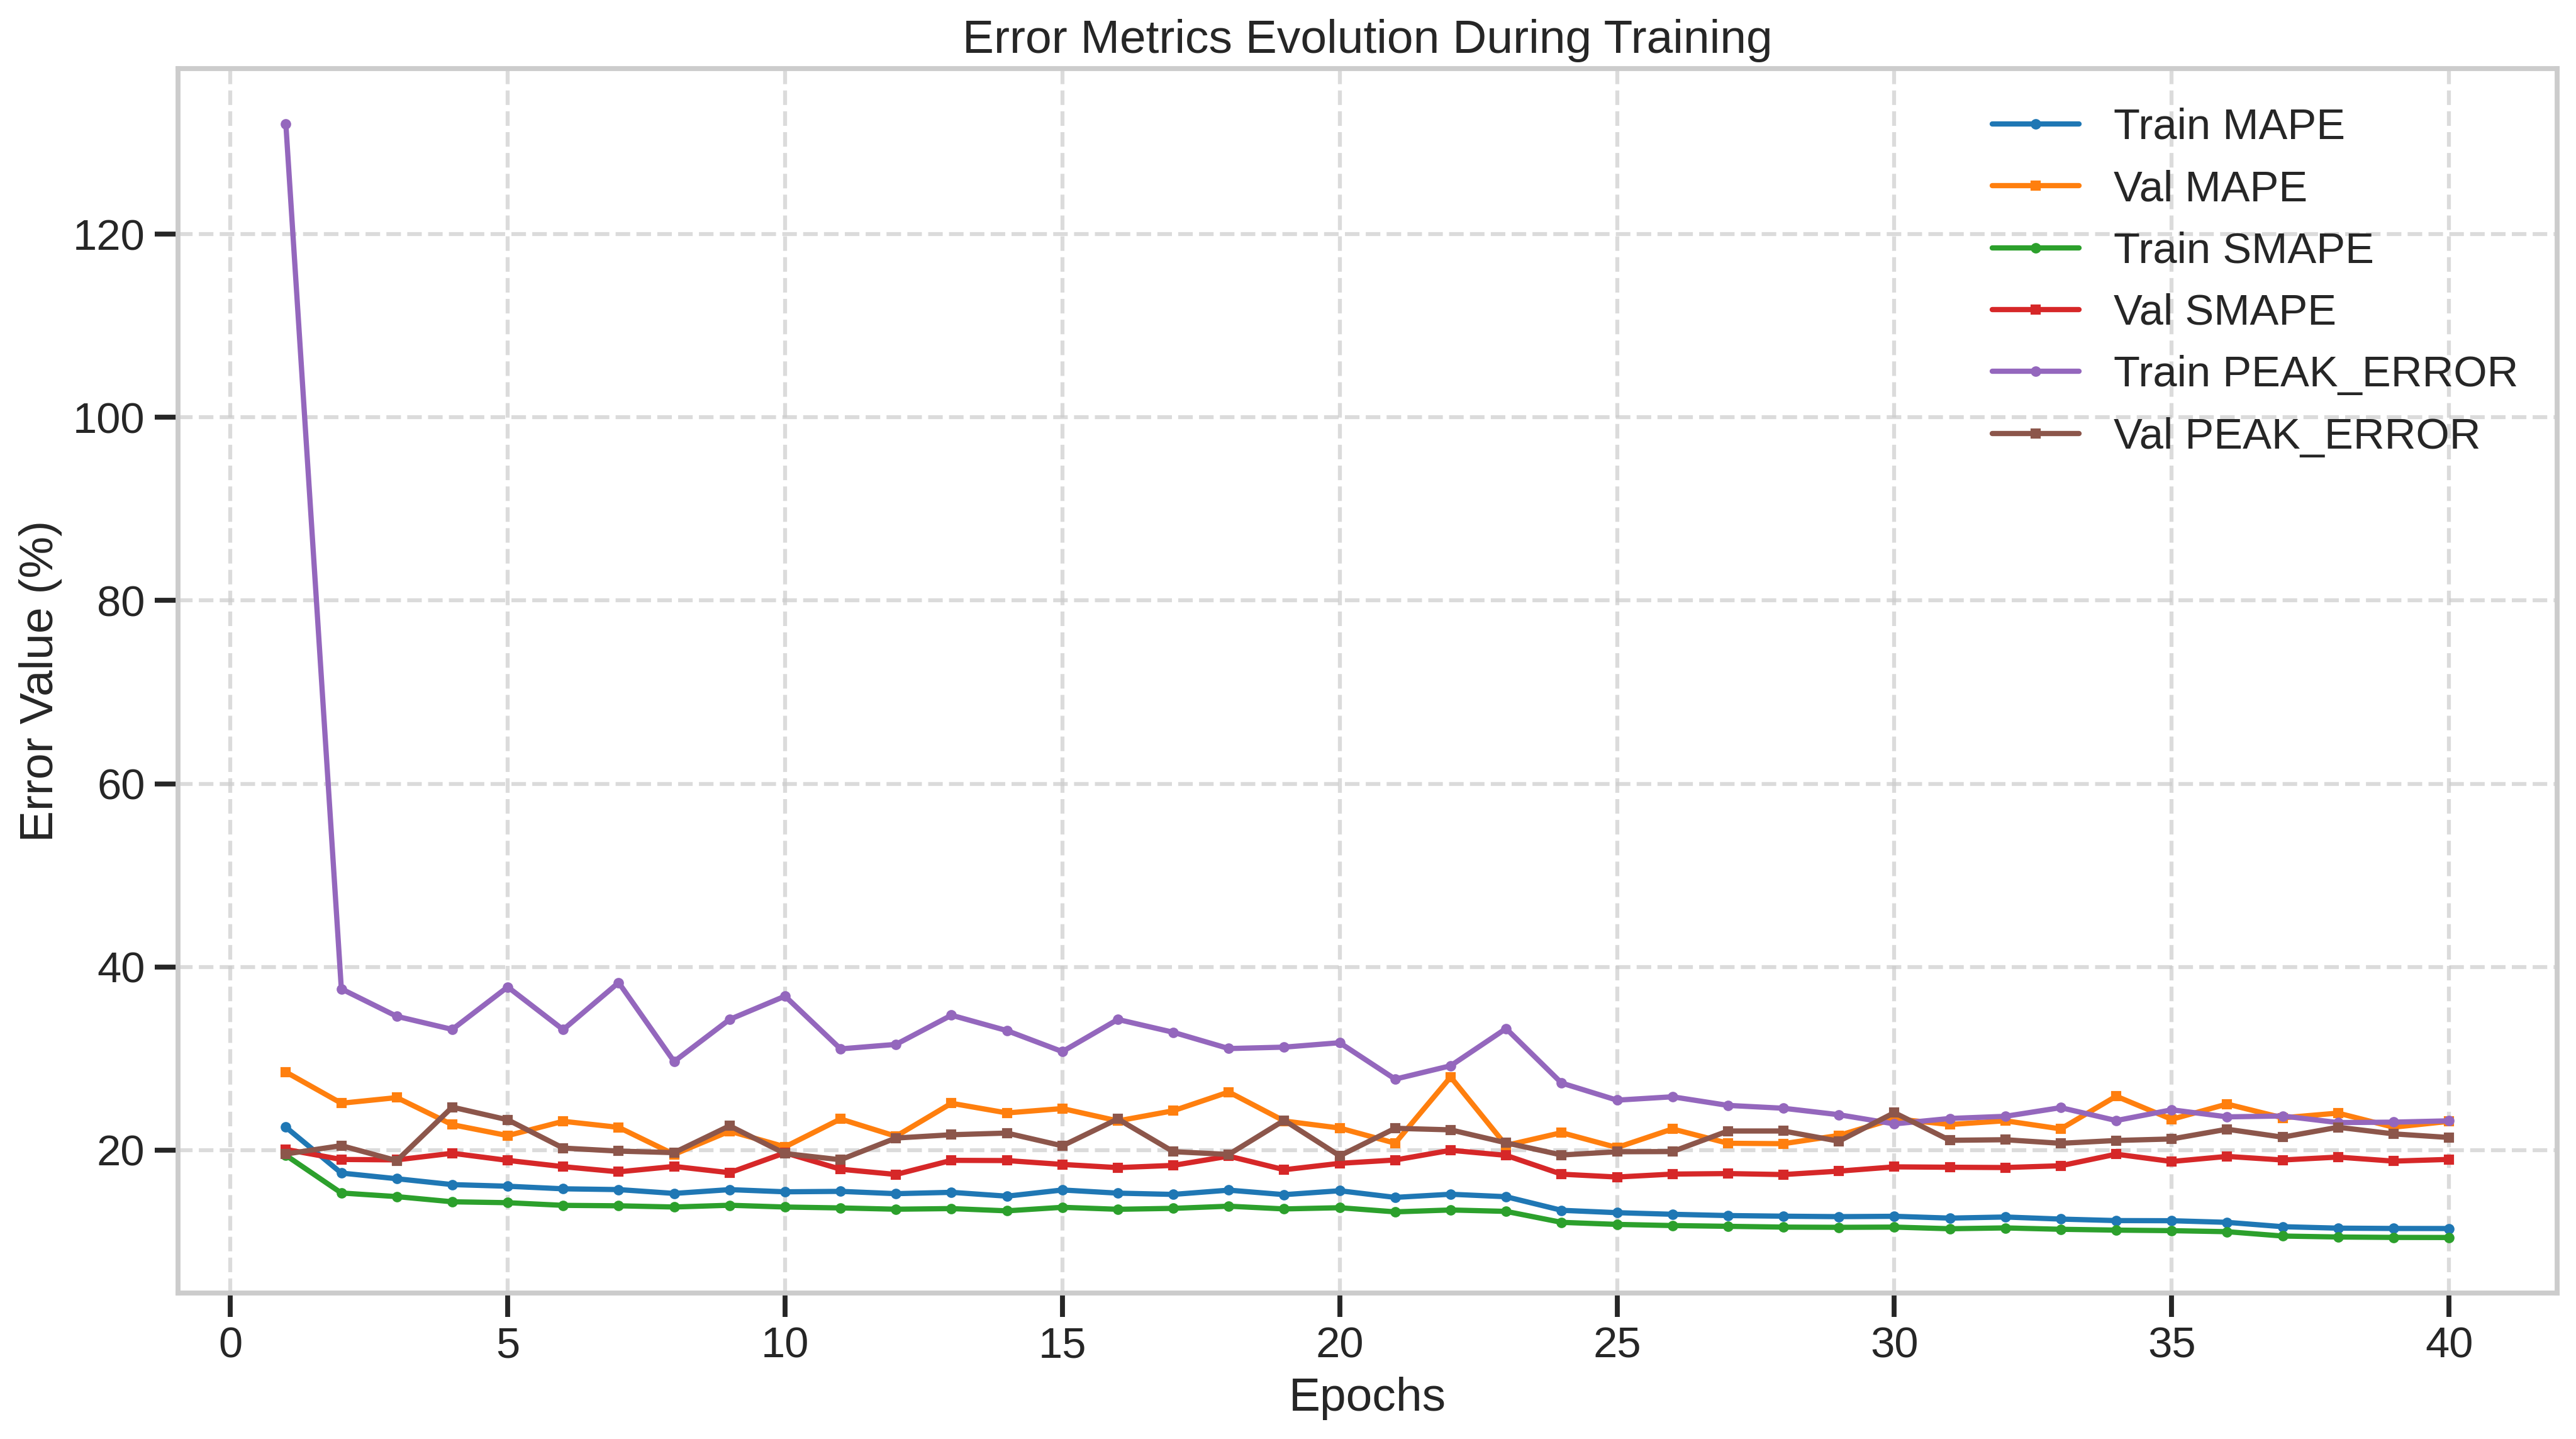
\includegraphics[width=\textwidth]{bestmodel_error_metrics_evolution.png}
\caption{Best model error metrics evolution}
\label{fig:bestmodel_error_metrics_evolution}
\end{figure}

Pri analýze výsledkov trénovania modelu s optimálnymi hyperparametrami bolo zistené, že dosiahnutá hodnota funkcie chyby bola nižšia v porovnaní s rovnakými hyperparametrami použitými počas fázy vyhľadávania.

\subsubsection{Dynamické prispôsobovanie učiacej rýchlosti}

Graf \textbf{Learning Rate Schedule} zobrazuje zmenu učiacej rýchlosti v priebehu tréningu. Použitie schémy adaptívneho zmenšovania učiacej rýchlosti (learning rate scheduler) po určitom počte epoch pomohlo modelu vyhnúť sa preškoleniu a zároveň optimalizovať konvergenciu.

\begin{figure}[ht!]
\centering
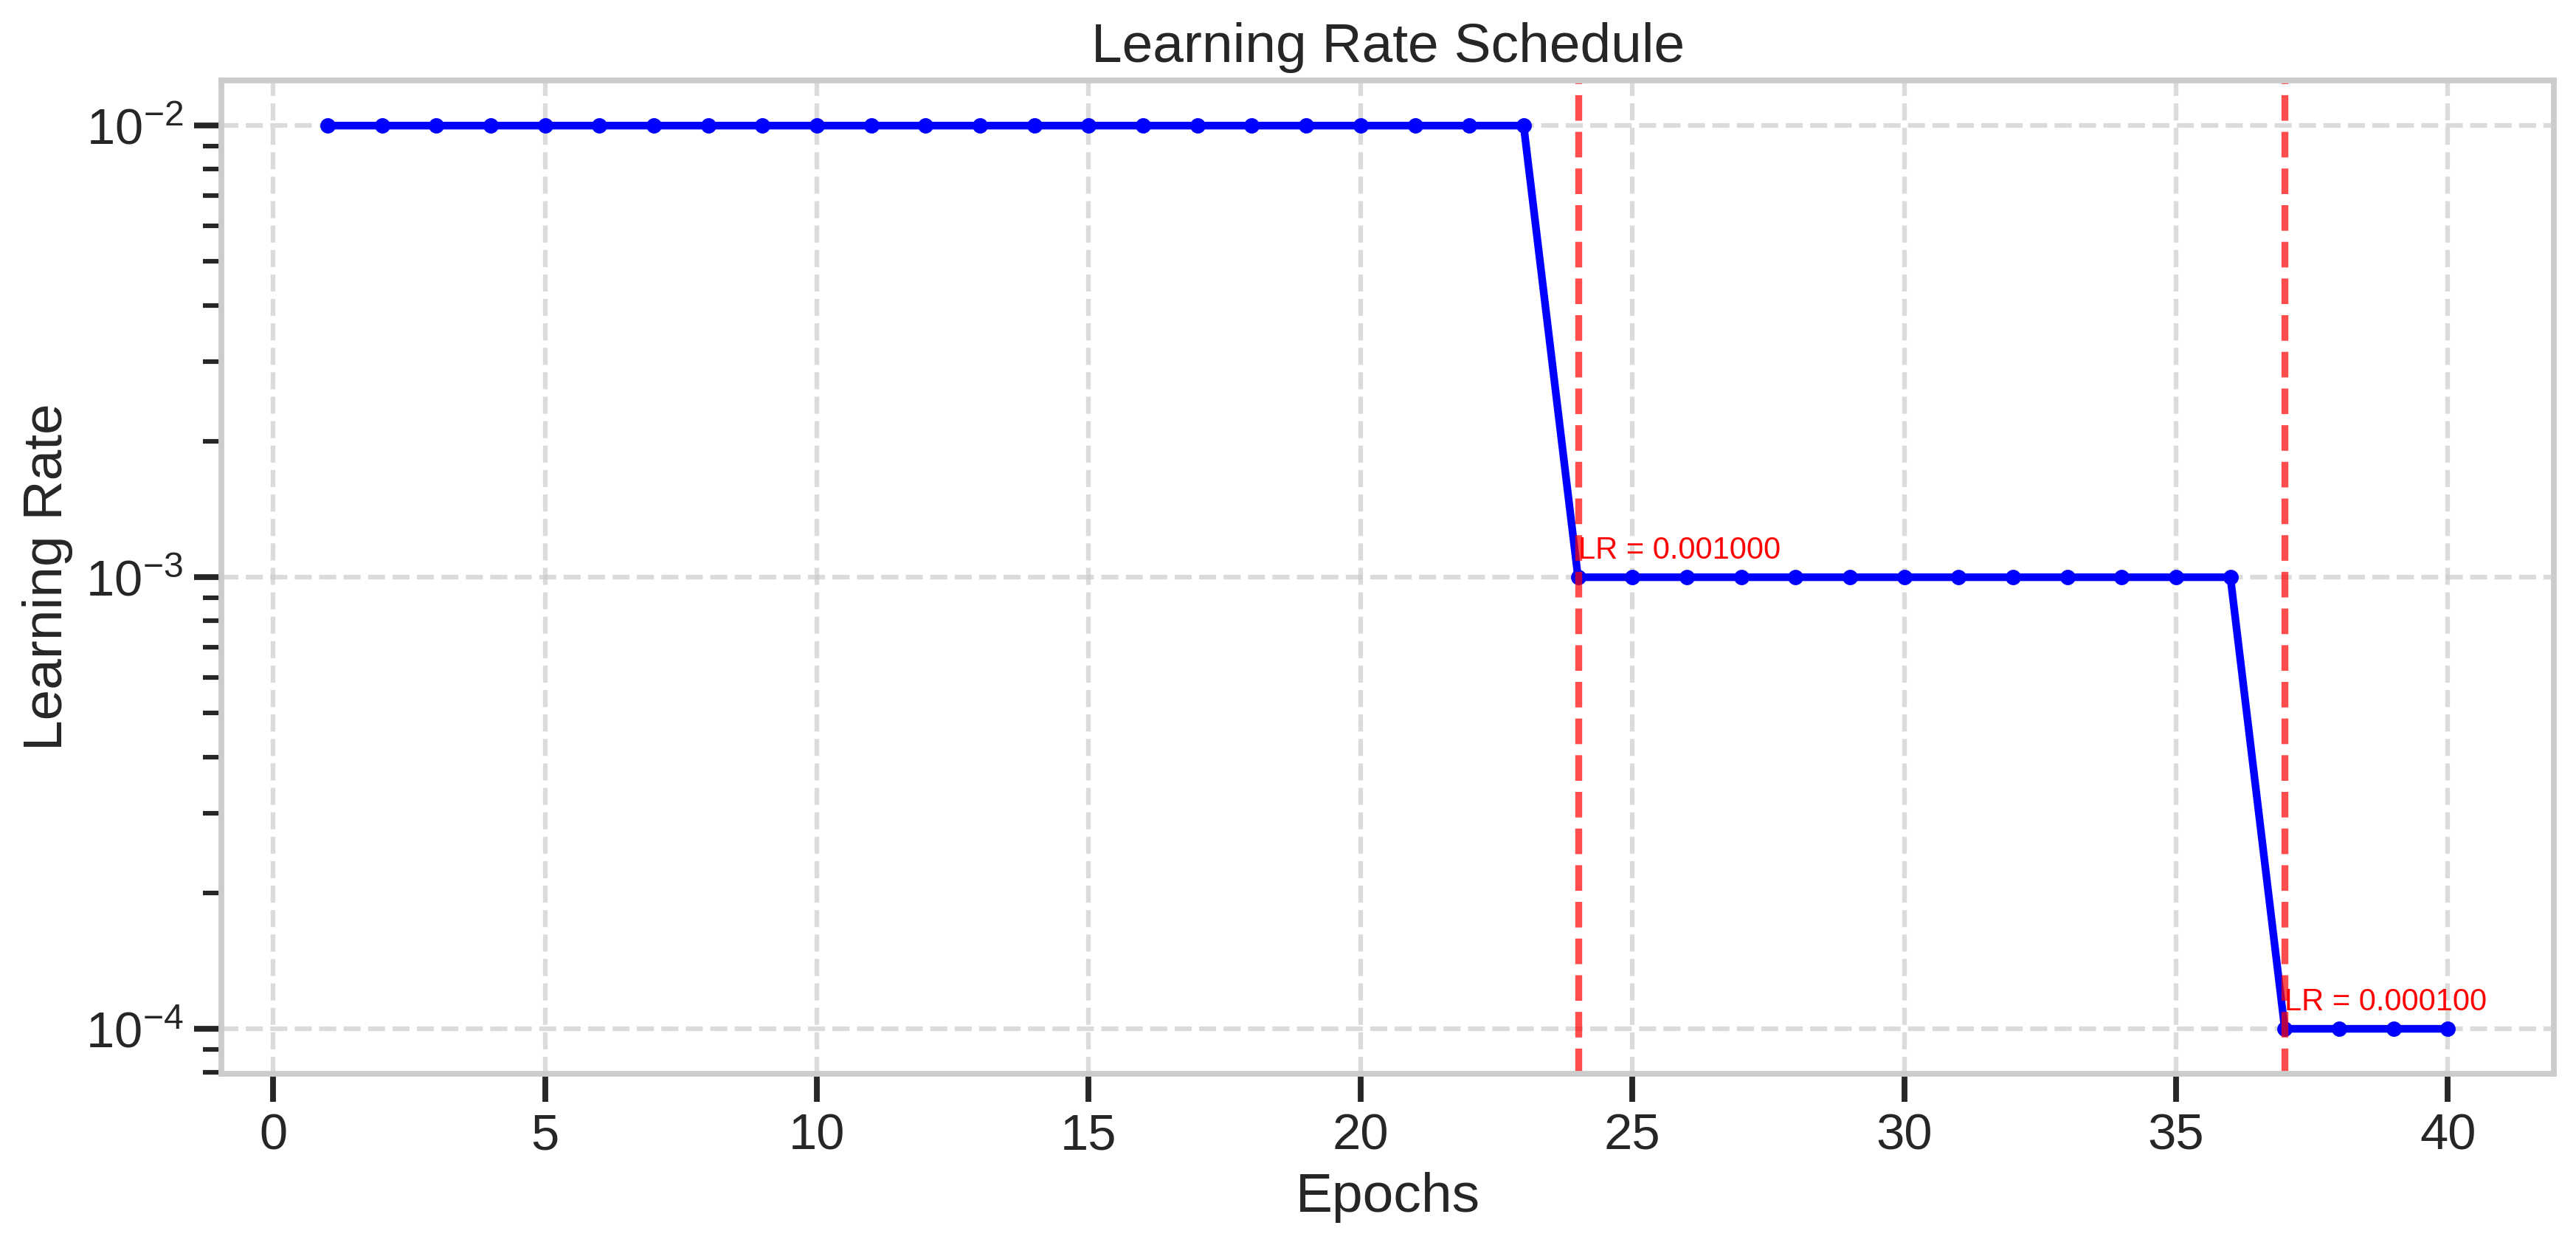
\includegraphics[width=\textwidth]{bestmodel_learning_rate_schedule.png}
\caption{Best model learning rate schedule}
\label{fig:bestmodel_learning_rate_schedule}
\end{figure}

\newpage

\subsubsection{Porovnanie tréningových a validačných metrík}

Na grafoch \textbf{Loss Train vs Validation}, \textbf{MAE Train vs Validation}, \textbf{R\textsuperscript{2} Train vs Validation} a \textbf{RMSE Train vs Validation} je jasne vidieť, že medzi trénovacou a validačnou sadou nie je zjavný overfitting. Hodnoty R\textsuperscript{2} \ref{r2} a RMSE \ref{rmse} ukazujú na vysokú presnosť modelu pri predikcii.

\begin{figure}[ht!]
    \centering
    \begin{subfigure}[b]{0.49\textwidth}
        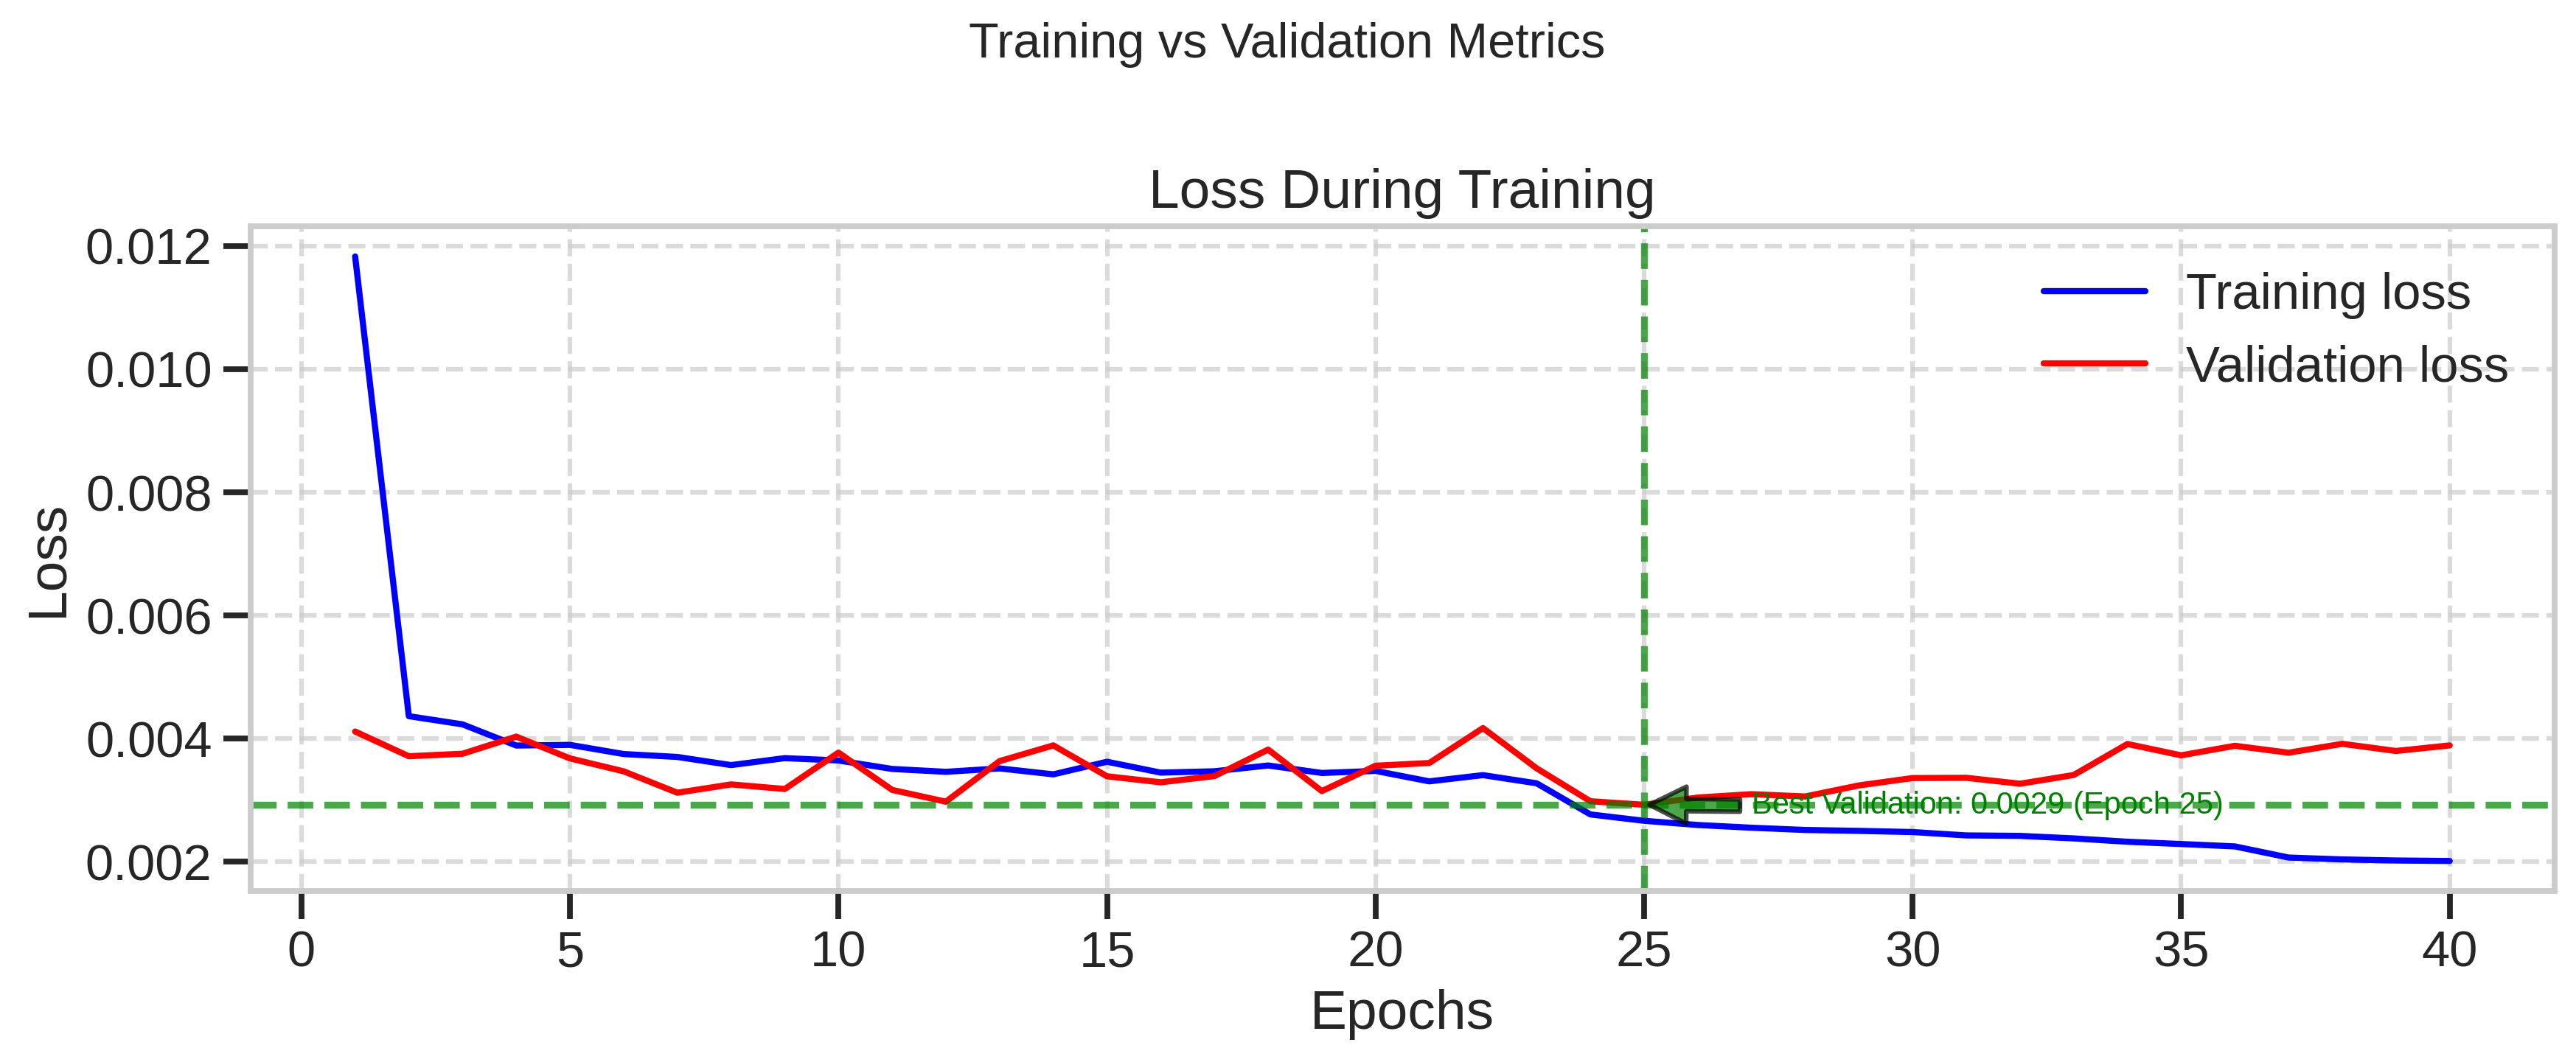
\includegraphics[width=\textwidth]{bestmodel_loss_train_val_comparison.png}
        \caption{Loss train vs validation}
        \label{fig:bestmodel_loss_train_val_comparison}
    \end{subfigure}
    \hfill
    \begin{subfigure}[b]{0.49\textwidth}
        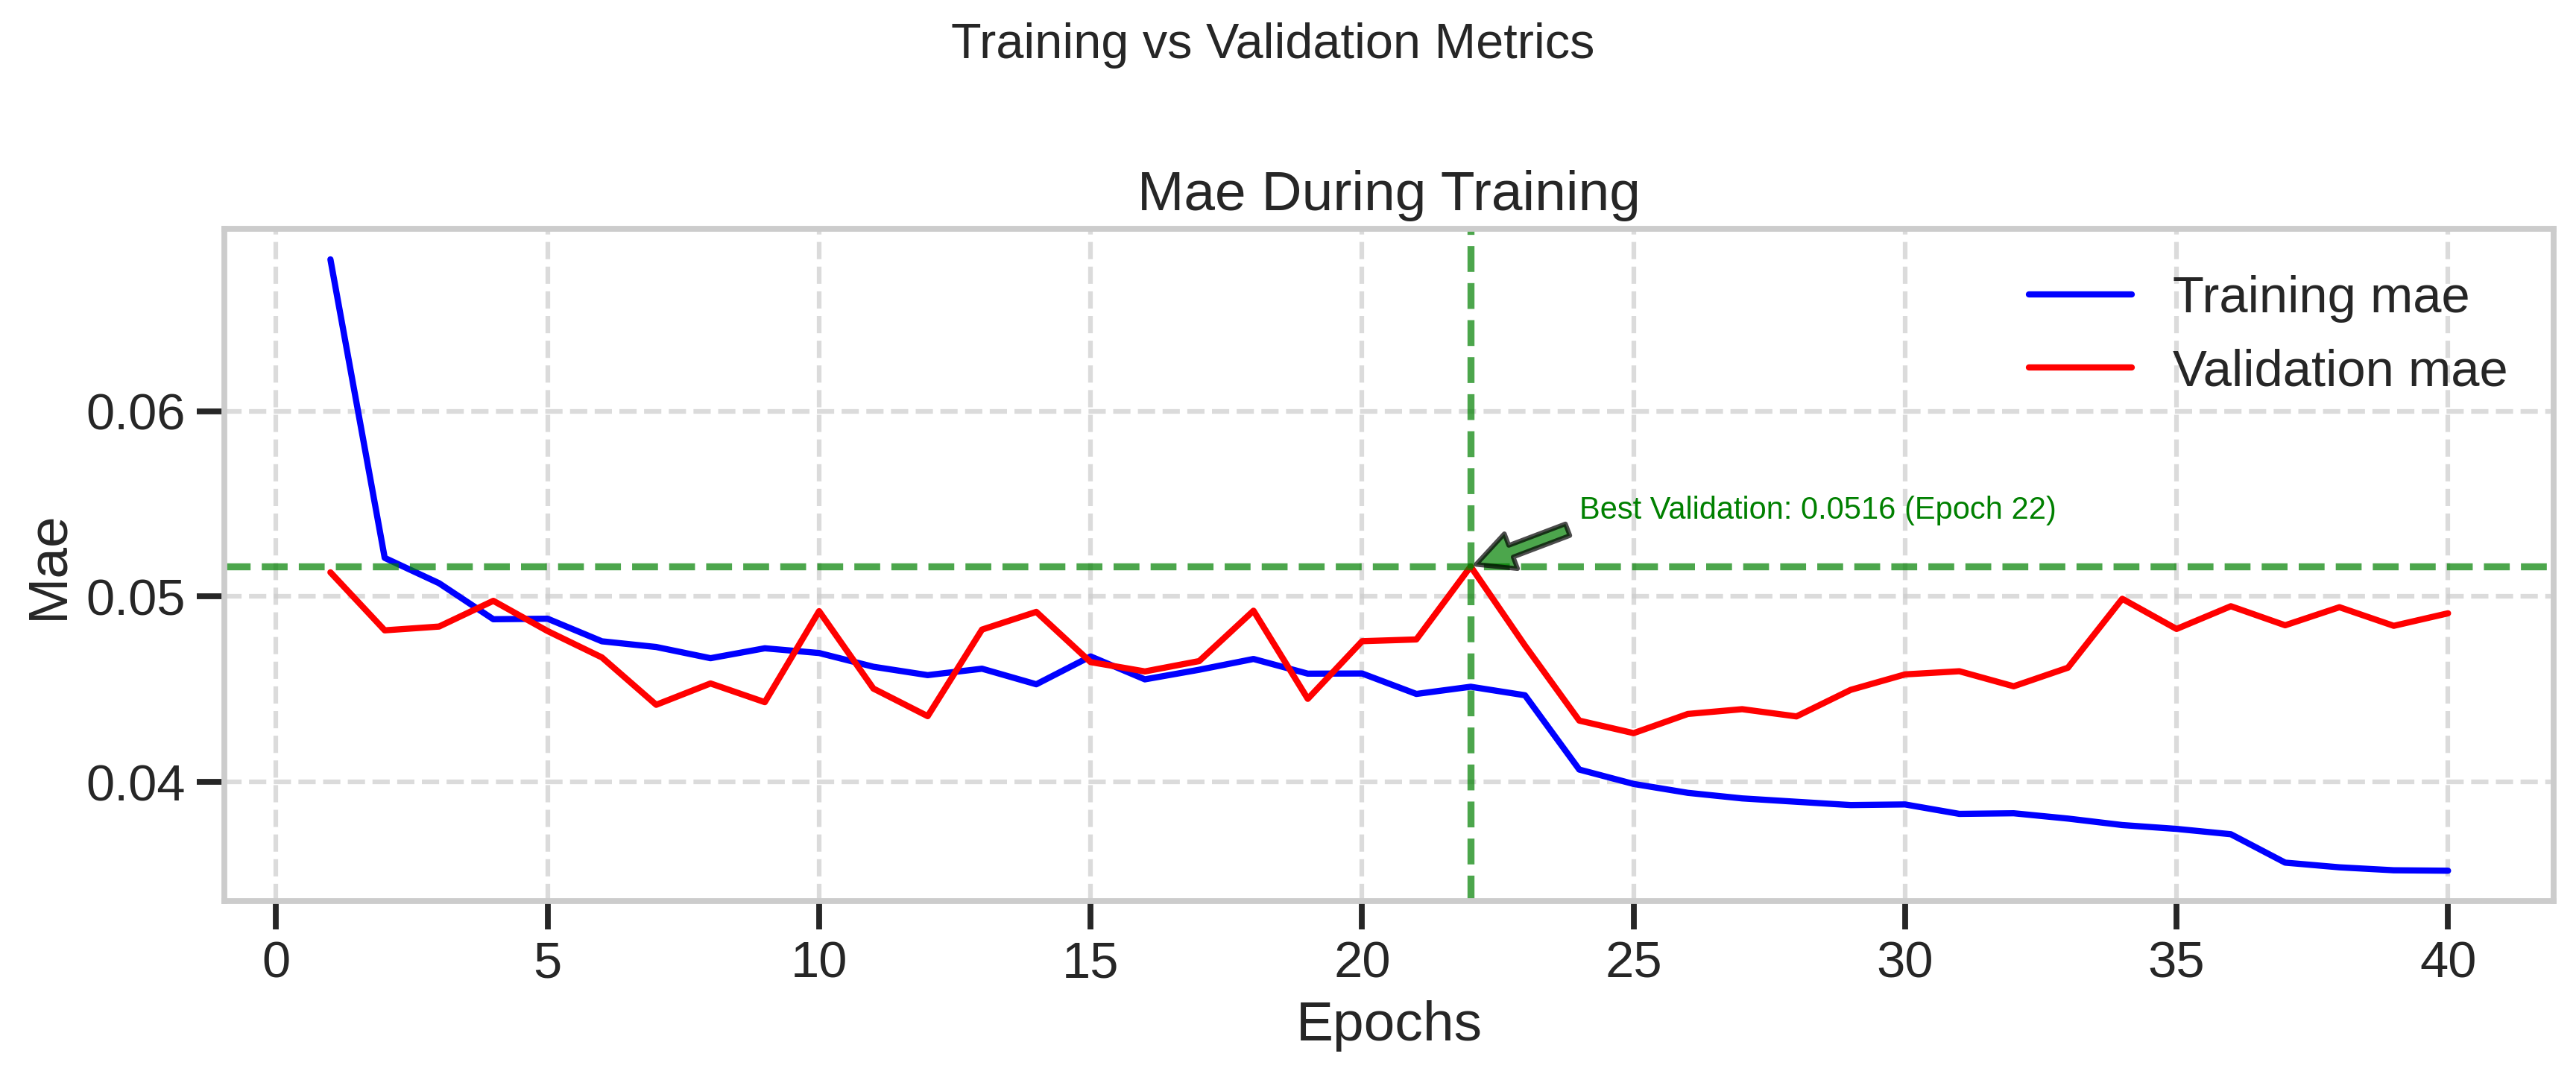
\includegraphics[width=\textwidth]{bestmodel_mae_train_val_comparison.png}
        \caption{MAE train vs validation}
        \label{fig:bestmodel_mae_train_val_comparison}
    \end{subfigure}
    \vskip\baselineskip
    \begin{subfigure}[b]{0.49\textwidth}
        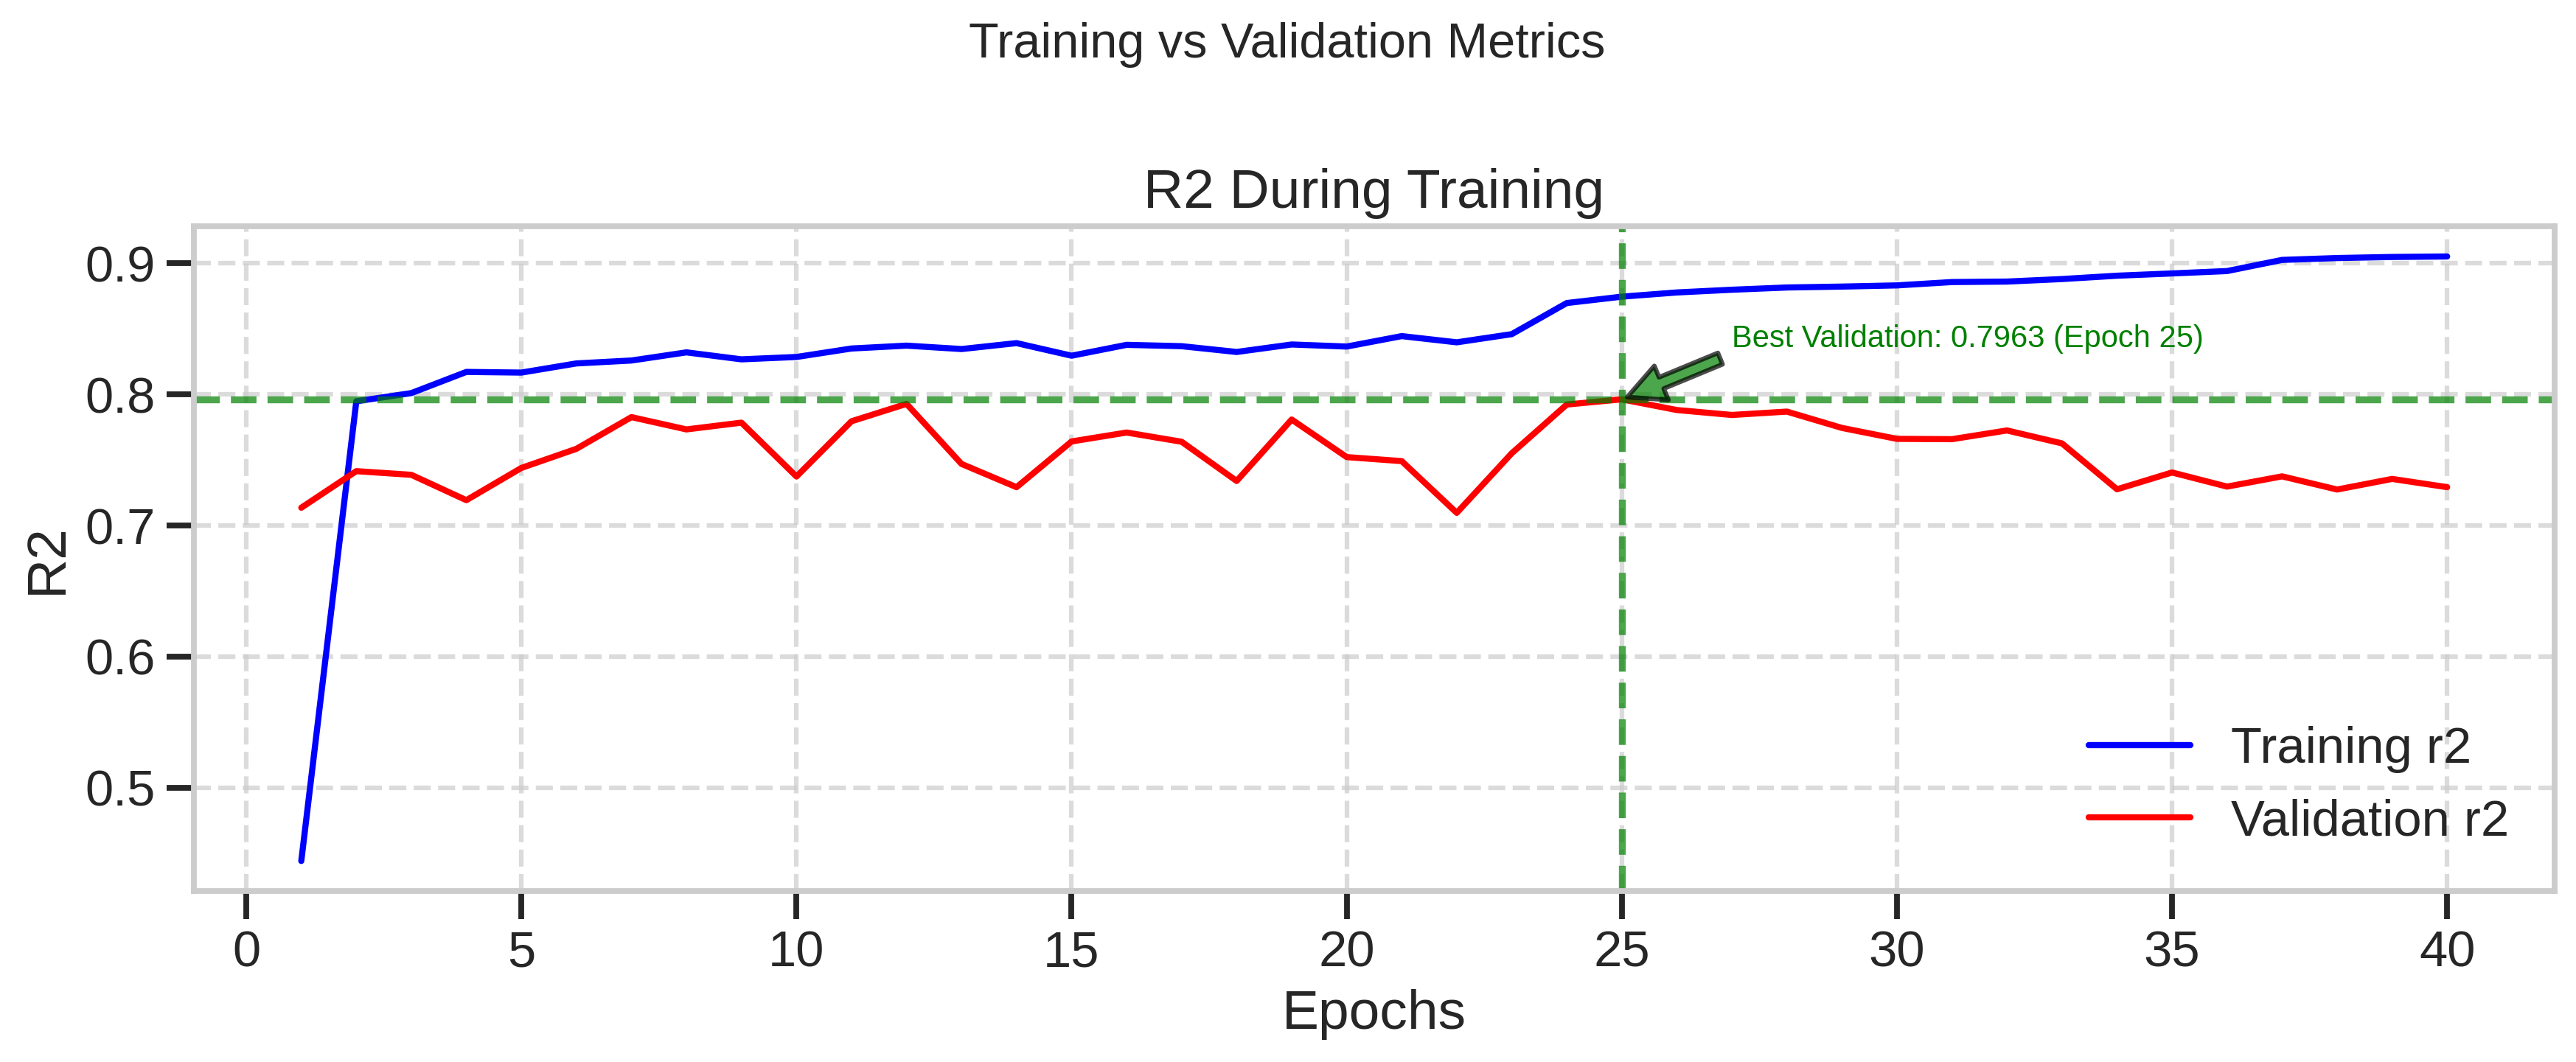
\includegraphics[width=\textwidth]{bestmodel_r2_train_val_comparison.png}
        \caption{R2 train vs validation}
        \label{fig:bestmodel_r2_train_val_comparison}
    \end{subfigure}
    \hfill
    \begin{subfigure}[b]{0.49\textwidth}
        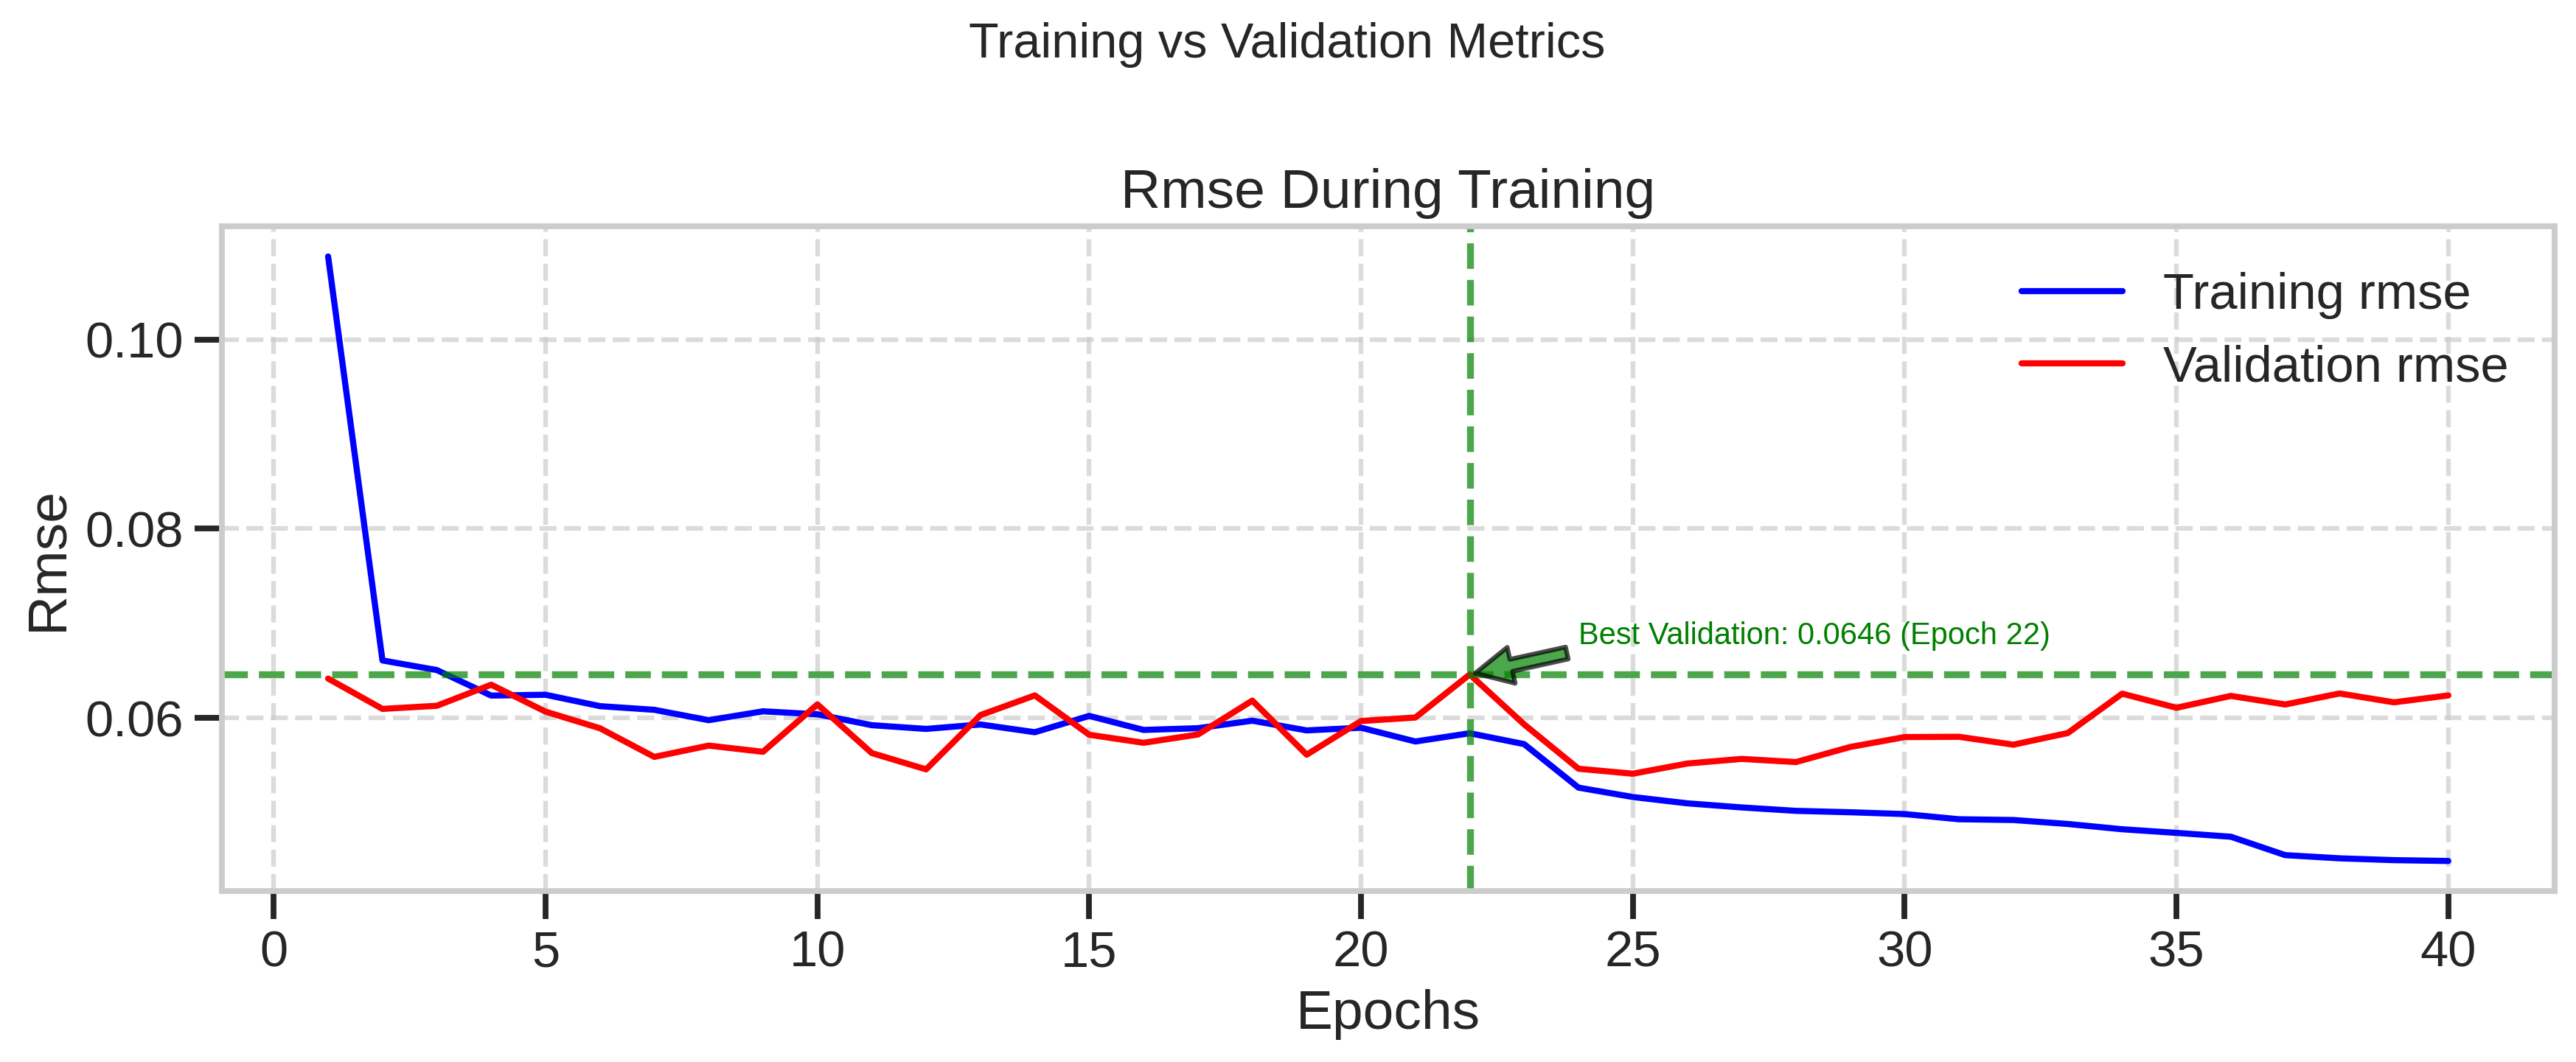
\includegraphics[width=\textwidth]{bestmodel_rmse_train_val_comparison.png}
        \caption{RMSE train vs validation}
        \label{fig:bestmodel_rmse_train_val_comparison}
    \end{subfigure}
    \caption{Best model training and validation metrics comparison}
    \label{fig:bestmodel_metrics_comparison}
\end{figure}

\newpage

\subsubsection{Komplexná metrická vizualizácia}

Radarový graf \textbf{Model Performance Radar Chart} sumarizuje výkonnostné metriky modelu na poslednej epoche, čo poskytuje intuitívny prehľad o rovnováhe medzi jednotlivými chybami (MAE \ref{mae}, RMSE \ref{rmse}, MAPE \ref{mape}, SMAPE \ref{smape}, R\textsuperscript{2} \ref{r2}, Explained Variance \ref{ev}, Peak Error \ref{pe}).

\begin{figure}[ht!]
\centering
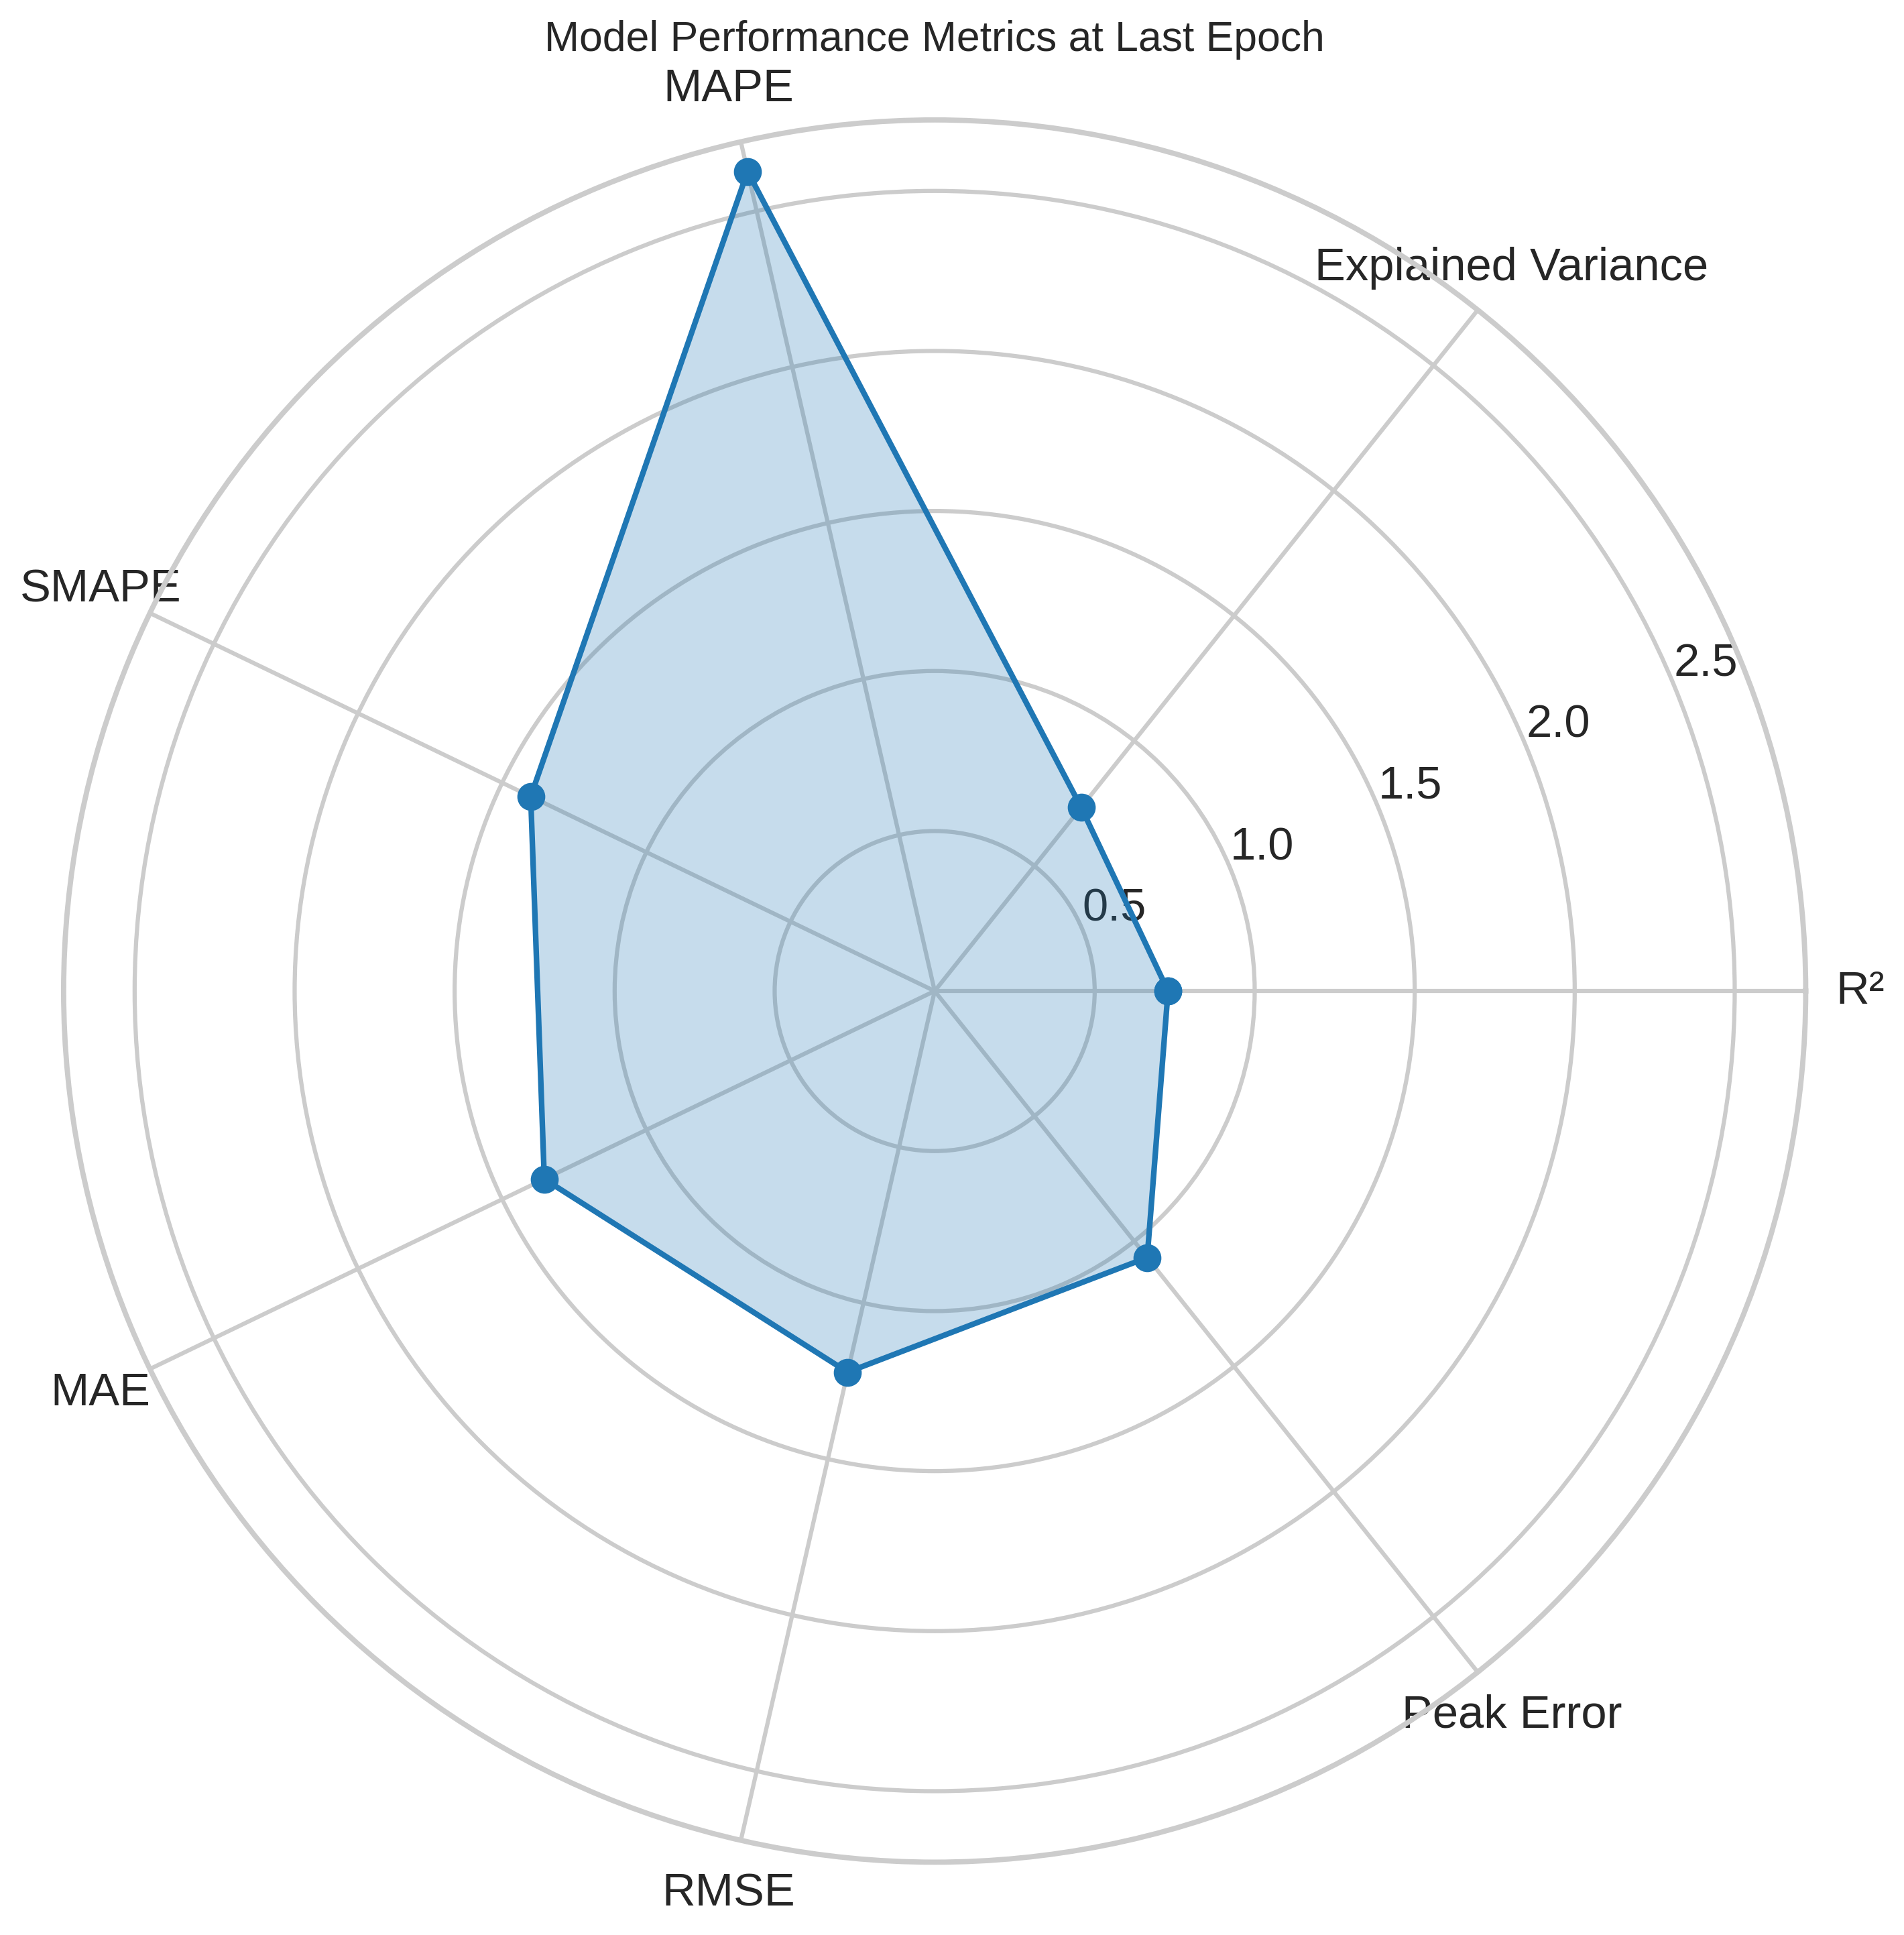
\includegraphics[width=0.8\textwidth]{bestmodel_model_radar_chart.png}
\caption{Best model radar chart}
\label{fig:bestmodel_radar_chart}
\end{figure}

\newpage

\subsubsection{Porovnanie výkonu modelu v priebehu epoch}

Na viacrozmerných krivkách \textbf{Metrics Comparison Over Epochs} je možné sledovať paralelne vývoj stratovej funkcie a výkonu (R\textsuperscript{2} \ref{r2}) v priebehu epoch. Model preukázal stabilný rast presnosti a pokles chyby bez znakov divergencie.

\begin{figure}[ht!]
\centering
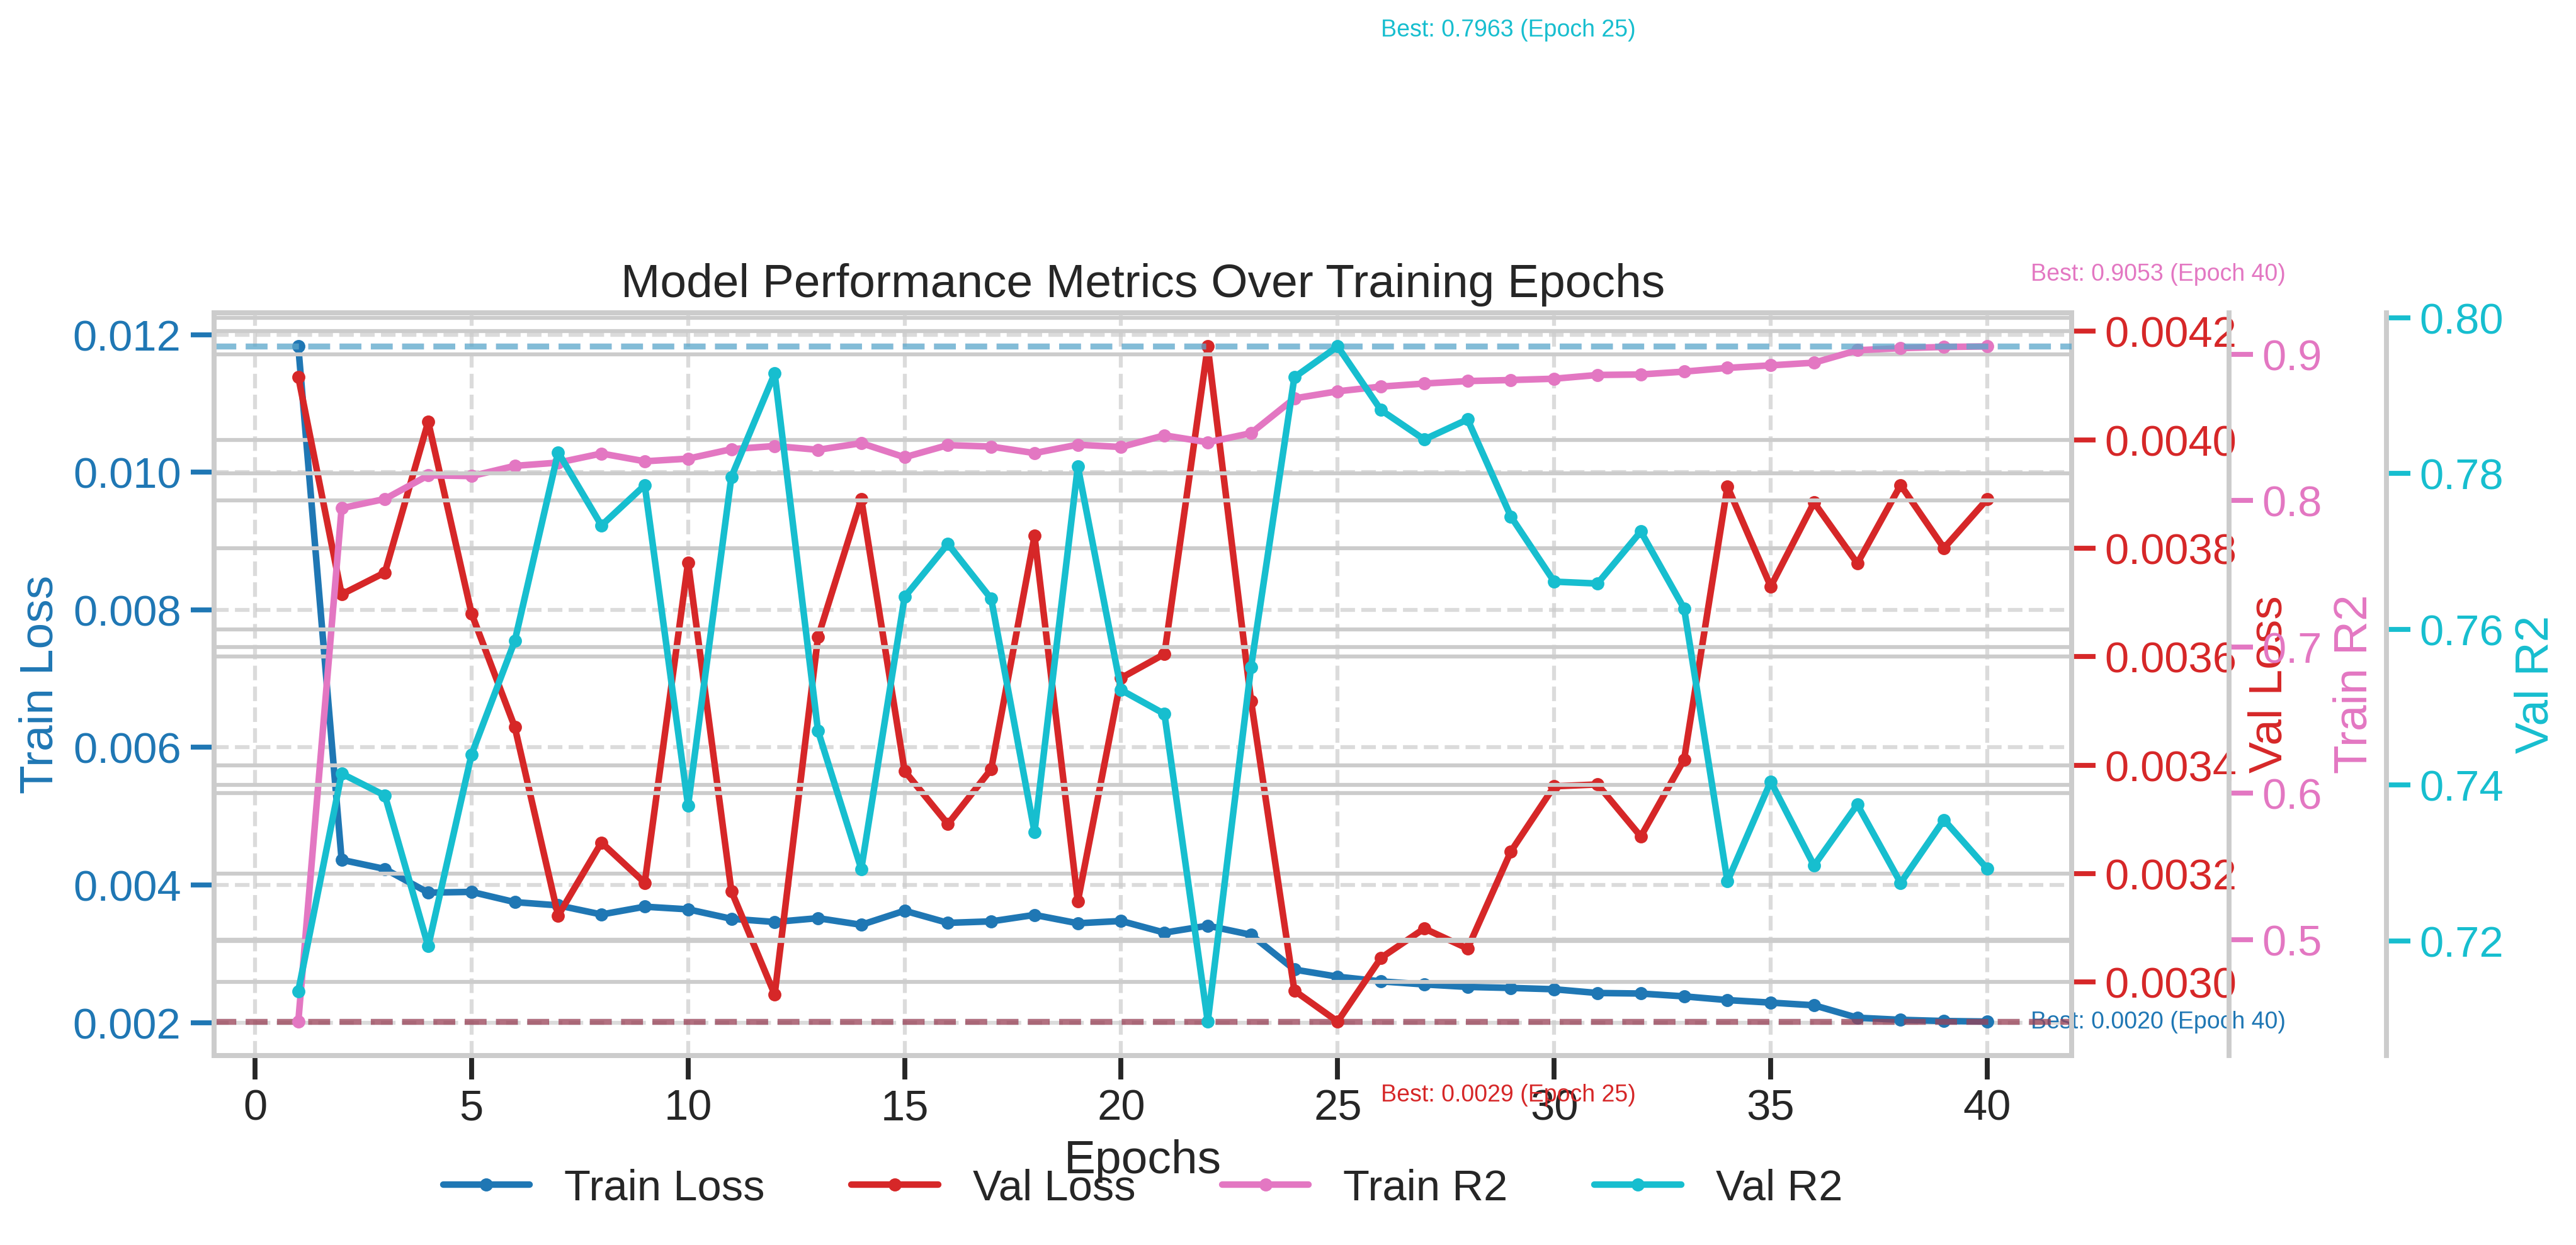
\includegraphics[width=\textwidth]{bestmodel_metrics_comparison.png}
\caption{Metrics comparison over epochs}
\label{fig:bestmodel_metrics_comparison}
\end{figure}

Detailnou analýzou grafu možno pozorovať, že iba v záverečných fázach tréningu sa objavuje mierne rozbiehanie validačných metrík. Tento jav môže indikovať začínajúci sa proces pretrénovania modelu, hoci divergencia nie je výrazná. Takáto tendencia naznačuje, že model postupne stráca svoju generalizačnú schopnosť a začína sa príliš špecializovať na trénovacie dáta.

Sumarizujúc výsledky experimentov, optimalizovaný GRU model vykazuje vynikajúce prediktívne schopnosti s vysokou presnosťou na validačnej množine. Použitie early stopping mechanizmu zabezpečilo, že model bol zastavený v optimálnom bode pred výrazným prejavom pretrénovania, čo potvrdzuje efektívnosť zvoleného prístupu k optimalizácii hyperparametrov a tréningu modelu.
% \section{Z\'aver (zhodnotenie rie\v{s}enia)}
% 
% Táto časť\/ záverečnej práce je povinná. Autor uvedie zhodnotenie
% riešenia. Uvedie výhody, nevýhody riešenia,  použitie výsledkov, ďalšie
% možnosti a~pod., prípadne načrtne iný spôsob riešenia úloh, resp.
% uvedie, prečo postupoval uvedeným spôsobom.
%  
% 
% Na strane \pageref{o:nlp} Vám ukážem ako sa používajú citácie.
% Ukážka:
% 
% \cite{Sumichrast2013}
% 
% \citep{Sumichrast2013}
% 
% \citealt{Sumichrast2013}
% 
% \citeyear{Sumichrast2013}
% 
% \citeauthor{Sumichrast2013}


% \begin{figure}
% \centering
% \includegraphics[width=.95\textwidth,angle=0]{natlib.PNG}
% \caption{Ukážka použitia \texttt{natlib package}}\label{o:nlp}
% \end{figure}

\section{Záver}

Cieľom tejto práce bolo navrhnúť, implementovať a vyhodnotiť optimalizačný rámec pre model GRU, ktorý umožňuje efektívnu predikciu na základe časových radov. V priebehu riešenia sme aplikovali tri rôzne prístupy k optimalizácii hyperparametrov: Random Search, Bayesian Search a Grid Search. Finálna verzia modelu bola trénovaná s využitím najlepšej kombinácie hyperparametrov získaných z Grid Search. Následná analýza preukázala vysokú generalizačnú schopnosť a stabilitu modelu.

\subsection{Zhrnutie dosiahnutých výsledkov}

\begin{itemize}
\item Bol navrhnutý a implementovaný univerzálny rámec pre hľadanie optimálnych hyperparametrov GRU modelov.
\item Vyvinutý model dosiahol výborné výsledky na reálnej dátovej množine (požičky bicyklov v Londýne).
\item Získané výsledky boli dôkladne analyzované pomocou metrických ukazovateľov (RMSE, MAE, R\textsuperscript{2}, MAPE, SMAPE, atď.).
\item Bola overená účinnosť kombinovaného prístupu k optimalizácii – Random a Bayesian Search na zúženie priestoru a Grid Search pre detailné ladenie.
\item Najlepší model dosiahol hodnotu R\textsuperscript{2} = 0.83122 na validačnej množine, čo predstavuje vysoko presný výsledok vzhľadom na komplexnosť úlohy.
\end{itemize}

\subsection{Hodnotenie kvality riešenia}

Model vykazuje:

\begin{itemize}
\item Rýchlu konvergenciu počas trénovania bez známok výrazného overfittingu.
\item Stabilitu počas celého tréningového procesu.
\item Výborný súlad medzi trénovacou a validačnou množinou.
\item Robustnosť voči výkyvom v dátach, ako ukazujú metriky PEAK ERROR a SMAPE.
\end{itemize}

Zvolený prístup sa ukázal ako efektívny a prakticky realizovateľný aj pri obmedzených výpočtových zdrojoch, najmä vďaka kombinácii adaptívnych a systematických metód optimalizácie.

\subsection{Odporúčania a návrhy na zlepšenie}

\begin{itemize}
\item Rozšíriť množinu testovaných metód o ďalšie optimalizačné techniky ako napr. Tree-structured Parzen Estimator (TPE) alebo Hyperband.
\item Preskúmať vplyv iných architektúr (napr. LSTM) pre porovnanie s GRU.
\item Implementovať možnosti automatickej predikcie na produkčné dáta v reálnom čase.
\end{itemize}

\subsection{Záverečné zhodnotenie}

Zvolený prístup bol v praxi úspešný a viedol k vytvoreniu predikčného systému, ktorý je nielen presný, ale aj stabilný a efektívne navrhnutý. Model GRU trénovaný na optimalizovanej sade hyperparametrov dosiahol veľmi dobré výsledky a preukázal potenciál využitia pri predikcii časových radov v rôznych doménach. Celý vývojový cyklus — od analýzy problému cez výber metód, implementáciu, optimalizáciu až po vizualizáciu a vyhodnotenie — bol realizovaný systematicky a metodicky správne.


% ak chcete pouzivat Mendeley -- BibTeX Entry odkaz vlozite do literatura.BIB. Viac o moznych styloch najdete na http://www.cs.stir.ac.uk/~kjt/software/latex/showbst.html


\bibliographystyle{plain}
\begin{thebibliography}{99}

\bibitem{Dataset}
  H.~Mavrodiev, “London Bike Sharing Dataset” Kaggle, 2025. 
  [Online]. Available: \url{https://www.kaggle.com/datasets/hmavrodiev/london-bike-sharing-dataset}

\bibitem{GitHub}
	\textit{Nikita Chernysh}, “bike-gru-experiments” GitHub, 2025. 
	[Online]. Available: \url{https://github.com/kitnew/bike-gru-experiments}

\bibitem{PyTorch}
  A.~Paszke \textit{et al.}, “PyTorch: An imperative style, high-performance deep learning library,” 
  in \textit{Advances in Neural Information Processing Systems}, vol.~32, 2019.

\bibitem{GridSearch}
	\url{https://www.sciencedirect.com/topics/mathematics/grid-search}, "Grid Search"
	in \textit{Journal of Mathematical Psychology, 2013"}, \textit{Jay I. Myung a, Daniel R. Cavagnaro b, Mark A. Pitt a \textit{et al.}}.
	Available at: \url{https://doi.org/10.1016/j.jmp.2013.05.005}
\bibitem{RandomSearch}
	\url{https://www.sciencedirect.com/topics/engineering/random-search-method}, "Random Search Method"
	in \textit{Energy Conversion and Management, 2016}, \textit{Houssein Al Moussawi a b, Farouk Fardoun a, Hasna Louahlia-Gualous b \textit{et al.}}.
	Available at: \url{https://doi.org/10.1016/j.enconman.2016.04.085}
\bibitem{BayesianSearch}
	H. Alibrahim and S. A. Ludwig, "Hyperparameter Optimization: Comparing Genetic Algorithm against Grid Search and Bayesian Optimization," 2021 IEEE Congress on Evolutionary Computation (CEC), Kraków, Poland, 2021, pp. 1551-1559, doi: 10.1109/CEC45853.2021.9504761. keywords: {Training;Machine learning algorithms;Neural networks;Prediction algorithms;Search problems;Time measurement;Bayes methods;Hyperparmeter optimization;Grid Search;Bayesian;Genetic Algorithm},
	Available at: \url{https://ieeexplore.ieee.org/document/9504761}
\end{thebibliography}

\section*{Zoznam pr\'iloh}
\addcontentsline{toc}{section}{\numberline{}Zoznam pr\'iloh}
\thispagestyle{empty}

\begin{description}
	\item[Príloha A] Zdrojový kód
\end{description}
% !TeX root=tukedip.tex
% !TeX encoding = UTF-8
% !TeX spellcheck = sk_SK
\section*{Príloha A}
\addcontentsline{toc}{section}{\numberline{}Príloha A}
\subsection*{Prílohy}

\texttt{\href{https://github.com/kitne/bike-gru-experiments}{github.com/kitne/bike-gru-experiments}}

\end{document}